\newpage
\begin{center}
    \textbf{BAB IV} \\
    \textbf{HASIL DAN PEMBAHASAN}
    \addcontentsline{toc}{chapter}{BAB IV. HASIL DAN PEMBAHASAN}
\end{center}

\textbf{A. Data Uji Coba}
\addcontentsline{toc}{section}{A. Data Uji Coba}

\hspace*{1cm}Data uji coba dalam pengembangan media pembelajaran berbasis simulasi 3D pada materi bangun ruang untuk peserta didik kelas VIII SMP menggunakan model pengembangan ADDIE. Adapun tahapan dalam proses pengembangan meliputi Analisis (Analysis), Perancangan (Design), Pengembangan (Development), Implementasi (Implementation), dan Evaluasi (Evaluation).

\begin{enumerate}[leftmargin=1cm, label=\arabic*.]
    \item \textbf{Analisis}
    
    \hspace*{1cm}Tahap analisis adalah tahap awal dalam proses pengembangan pada penelitian ini. Pada tahap ini, peneliti melakukan analisis di SMP Muhammadiyah 9 Yogyakarta untuk mengetahui gambaran tentang media pembelajaran yang akan dikembangkan. Adapun analisis-analisis yang dilakukan antara lain:
    
    \begin{enumerate}[label=\textbf{\alph*.}]
        \item \textbf{Analisis Kebutuhan}
        
        \hspace*{1cm}Pada tahap ini, peneliti melakukan wawancara dengan guru matematika pada tanggal 28 April 2026, serta menyebarkan angket kepada peserta didik kelas VIII-B di SMP Muhammadiyah 9 Yogyakarta. Hasil penyebaran angket pra-penelitian disajikan pada Tabel~\ref{pra-penelitian}.
        
        \begin{table}[H]
            \centering
            \caption{Hasil penyebaran angket Pra-Penelitian Peserta Didik}
            \label{pra-penelitian}
            \begin{tabular}{|c|p{6cm}|>{\centering\arraybackslash}p{1.5cm}|>{\centering\arraybackslash}p{1.5cm}|}
                \hline
                \multirow{2}{*}{No} & \multirow{2}{*}{Indikator} & \multicolumn{2}{c|}{Respons Peserta Didik} \\
                \cline{3-4}
                & & Ya & Tidak \\
                \hline
                1 & Apakah pelajaran matematika sulit? & 84,4\% & 15,6\% \\
                \hline
                2 & Apakah materi bangun ruang sisi datar sulit dipahami? & 75\% & 25\% \\
                \hline
                3 & Saya lebih tertarik dengan pembelajaran praktik, daripada hanya dijelaskan oleh guru. & 62,5\% & 37,5\% \\
                \hline
                4 & Saya menyukai pendekatan pembelajaran yang membuat peserta didik menjadi lebih aktif. & 93,75\% & 6,25\% \\
                \hline
                5 & Saya menyukai pembelajaran dengan menggunakan teknologi. & 87,5\% & 12,5\% \\
                \hline
            \end{tabular}
        \end{table}

        \hspace*{1cm}Berdasarkan Tabel \ref{pra-penelitian} di atas, diperoleh data bahwa sebanyak 83,3\% peserta didik menganggap matematika sulit. Setelah melakukan penyebaran angket, peneliti juga melakukan wawancara kepada beberapa peserta didik. Hasil wawancara menunjukkan bahwa peserta didik mengalami kesulitan dalam menyelesaikan soal yang berkaitan dengan bangun ruang sisi datar. Hal ini disebabkan oleh kesulitan peserta didik dalam membayangkan bentuk bangun ruang tersebut. Hasil penyebaran angket dan wawancara disajikan sebagai berikut.

        \begin{enumerate}
            \item Sumber belajar yang digunakan dalam pembelajaran adalah buku LKS serta catatan dari guru.
    
            \item Model pembelajaran yang digunakan adalah metode ceramah dan tanya jawab.
    
            \item Peserta didik mengalami kesulitan dalam memahami materi bangun ruang sisi datar.
    
            \item Peserta didik menyukai pembelajaran yang memanfaatkan teknologi.
    
            \item Pendidik matematika kelas VIII-D SMP Muhammadiyah 9 Yogyakarta belum pernah menggunakan teknologi simulasi 3D dalam proses pembelajaran.
        \end{enumerate}

        \hspace*{1cm}Dari permasalahan di atas, agar peserta didik lebih tertarik dengan pelajaran matematika, khususnya pada materi bangun ruang sisi datar, peneliti berniat menguji kelayakan media pembelajaran berbasis simulasi 3D. Media pembelajaran ini diharapkan dapat membantu peserta didik dalam belajar serta menarik minat belajar mereka.

        \item \textbf{Analisis Materi}
        
        \hspace*{1cm}Pada tahap ini, peneliti menentukan materi yang akan dikembangkan berdasarkan hasil wawancara dengan pendidik matematika di SMP Muhammadiyah 9 Yogyakarta. Materi yang dipilih adalah Bangun Ruang Sisi Datar karena masih dianggap sulit oleh peserta didik, terutama dalam menyelesaikan soal gambar bangun ruang dan soal cerita. Materi ini dinilai cocok untuk dikembangkan dengan teknologi simulasi 3D.

        \item \textbf{Analisis Kurikulum}
        
        \hspace*{1cm}Peneliti melakukan analisis terhadap kurikulum matematika yang digunakan di SMP Muhammadiyah 9 Yogyakarta. Karena sekolah menerapkan Kurikulum Merdeka, materi pembelajaran dikembangkan sesuai dengan capaian pembelajaran Fase D untuk kompetensi geometri.

        \hspace*{1cm}Capaian pembelajaran Fase D Kurikulum Merdeka pada domain geometri yang menjadi acuan pengembangan media pembelajaran ini meliputi:
        \begin{enumerate}[label=\alph*)]
            \item Mengidentifikasi dan menganalisis sifat serta hubungan antar unsur bangun ruang sisi datar dan jaring-jaringnya.
            \item Menggunakan representasi visual, berupa gambar, model, dan simulasi, untuk memahami konsep bangun ruang.
            \item Menyelesaikan masalah kontekstual yang berkaitan dengan bangun ruang sisi datar menggunakan penalaran matematika.
            \item Mengkomunikasikan penjelasan matematis secara lisan atau tertulis terkait konsep dan proses penyelesaian masalah geometri.
        \end{enumerate}

        \hspace*{1cm}Dengan demikian, pengembangan media pembelajaran berbasis simulasi 3D diarahkan untuk membantu peserta didik mencapai capaian pembelajaran fase D dalam memahami bangun ruang sisi datar.
    \end{enumerate}
    \item \textbf{Perancangan (Design)}\\
    \hspace*{1cm}Tahap perancangan mencakup dua aspek utama, yaitu perancangan konten materi pembelajaran dan perancangan sistem perangkat lunak. Pada tahap ini, peneliti menyusun strategi untuk mengintegrasikan teknologi simulasi 3D ke dalam platform berbasis web agar dapat memenuhi tujuan pembelajaran yang telah ditetapkan. Mengingat media pembelajaran berbasis simulasi 3D masih merupakan inovasi baru dalam bidang pendidikan, proses perancangan didokumentasikan secara rinci dan sistematis. Dokumentasi ini dimaksudkan untuk memfasilitasi pemahaman mendalam dan memungkinkan replikasi serta pengembangan lebih lanjut oleh peneliti lain. Berikut adalah rincian dari masing-masing tahapan perancangan:
    \begin{enumerate}
        \item Perancangan Tujuan Pembelajaran \\
        \hspace*{1cm}Pada tahap ini, peneliti menentukan tujuan pembelajaran yang ingin dicapai melalui media pembelajaran berbasis simulasi 3D. Tujuan pembelajaran dirancang untuk mendukung capaian pembelajaran kurikulum dan meningkatkan pemahaman peserta didik terhadap materi bangun ruang sisi datar. Adapun tujuan pembelajaran yang telah ditetapkan adalah sebagai berikut:
        \begin{enumerate}
            \item Memahami konsep volume bangun ruang sisi datar dengan memanfaatkan simulasi 3D interaktif.
            \item Memahami konsep luas permukaan bangun ruang sisi datar dengan memanfaatkan simulasi 3D interaktif.
            \item Menyelesaikan masalah kontekstual yang berkaitan dengan bangun ruang dalam kehidupan sehari-hari.
            \item Mengidentifikasi unsur-unsur bangun ruang sisi datar serta hubungannya dengan jaring-jaring.
            \item Merekonstruksi jaring-jaring bangun ruang menggunakan media konkret seperti kertas karton.
        \end{enumerate}
        \item Perancangan Materi \\
        \hspace*{1cm}Materi pembelajaran disusun berdasarkan hasil analisis materi dan kebutuhan peserta didik. Ruang lingkup materi mencakup bangun ruang sisi datar, yaitu kubus, balok, prisma, dan limas. Struktur hirarki materi disajikan pada diagram berikut untuk memudahkan pemahaman konsep dan alur pembelajaran.
        \begin{figure}[H]
            \centering
            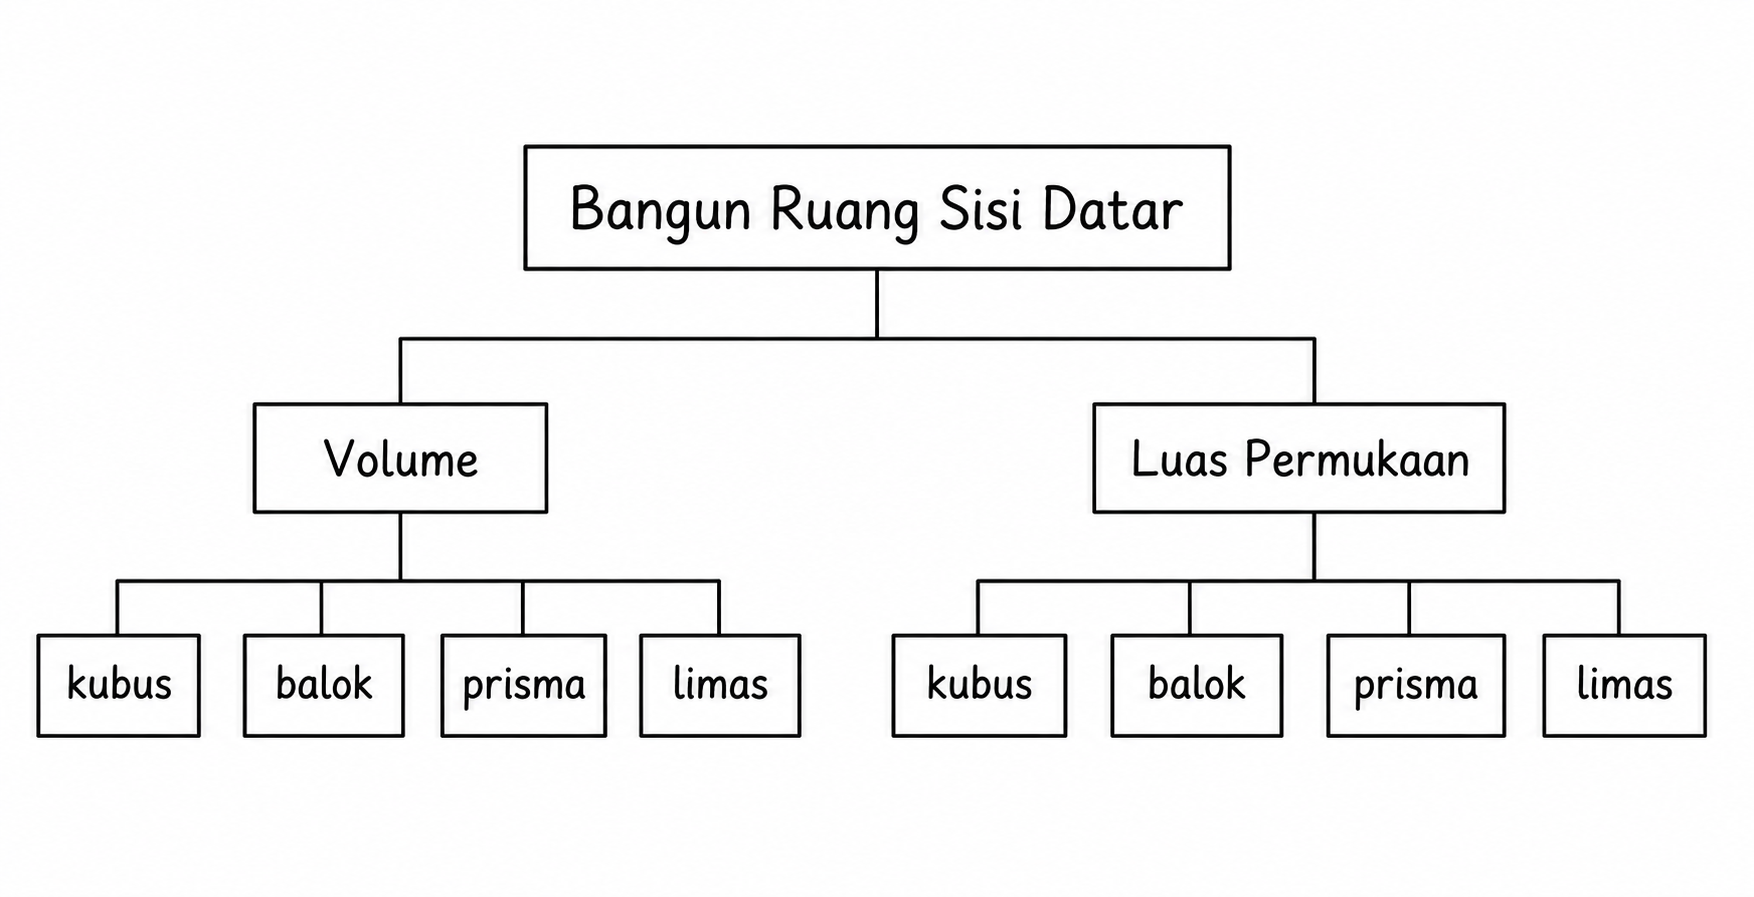
\includegraphics[width=0.8\textwidth]{images/bagan2.png}
            \caption{Struktur Hirarki Materi Bangun Ruang Sisi Datar}
            \label{fig:strukturmateri}
        \end{figure}
        Dari materi yang telah ditentukan, peneliti memilih beberapa materi yang dapat dijelaskan dengan simulasi 3D, yaitu:
        \begin{enumerate}[label=\arabic*.]
            \item Simulasi konsep volume pada kubus, menghitung banyaknya kubus satuan yang menyusun sebuah kubus.
            \item Simulasi konsep volume pada limas, sebuah kubus yang dapat berubah menjadi tiga buah limas dengan ukuran yang sama.
            \item Simulasi jaring-jaring bangun ruang kubus, balok, prisma, dan limas.
        \end{enumerate}
        \item Perancangan Media \\
        \hspace*{1cm}Terlebih dahulu peneliti merancang tampilan media dalam bentuk mockup. Mockup ini berfungsi sebagai prototipe awal untuk merancang antarmuka pengguna (UI) media pembelajaran berbasis simulasi 3D. Desain UI dirancang dengan mempertimbangkan aspek kegrafikan, kemudahan navigasi, dan keterlibatan pengguna. Berikut adalah contoh desain mockup yang telah dibuat.
        \begin{figure}[H]
            \centering
            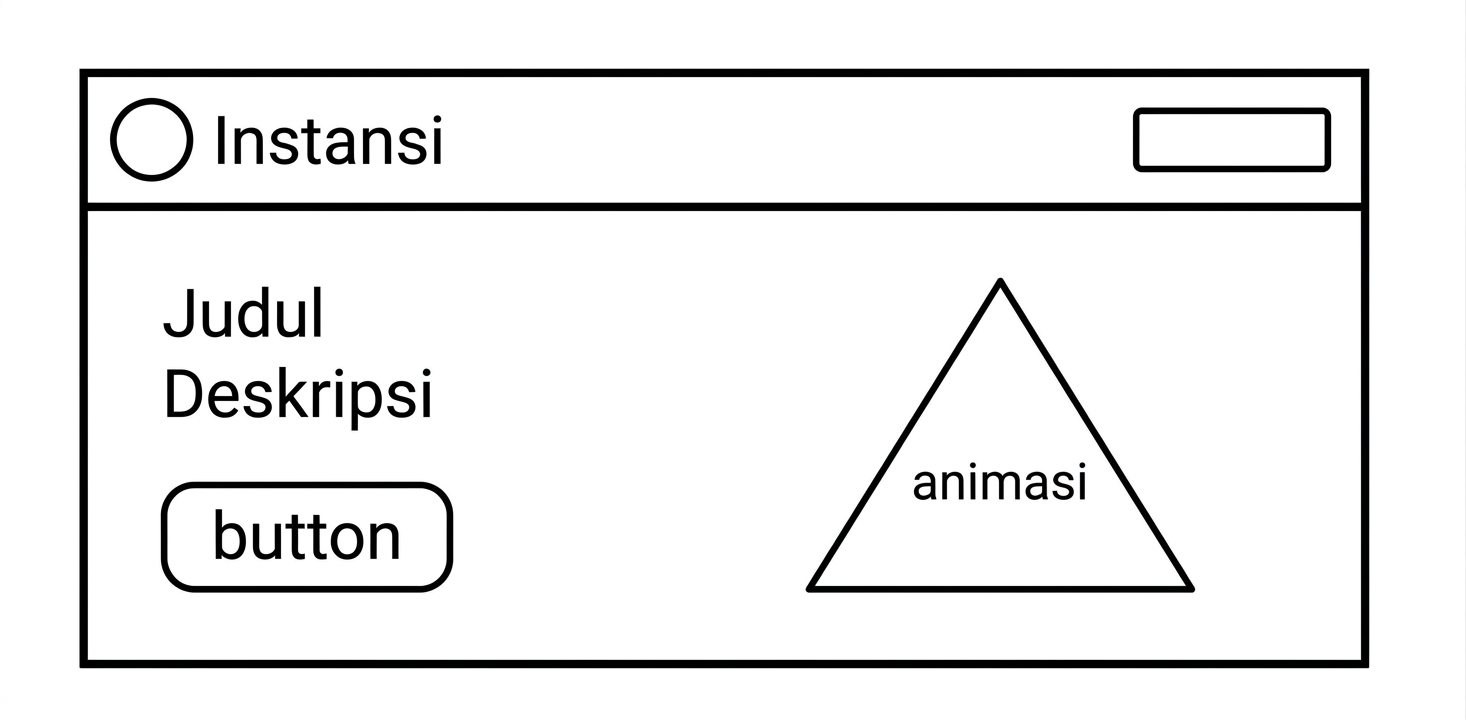
\includegraphics[width=0.8\textwidth]{images/landingpage2.png}
            \caption{Landing Page}
            \label{fig:landingpage}
        \end{figure}
        \begin{figure}[H]
            \centering
            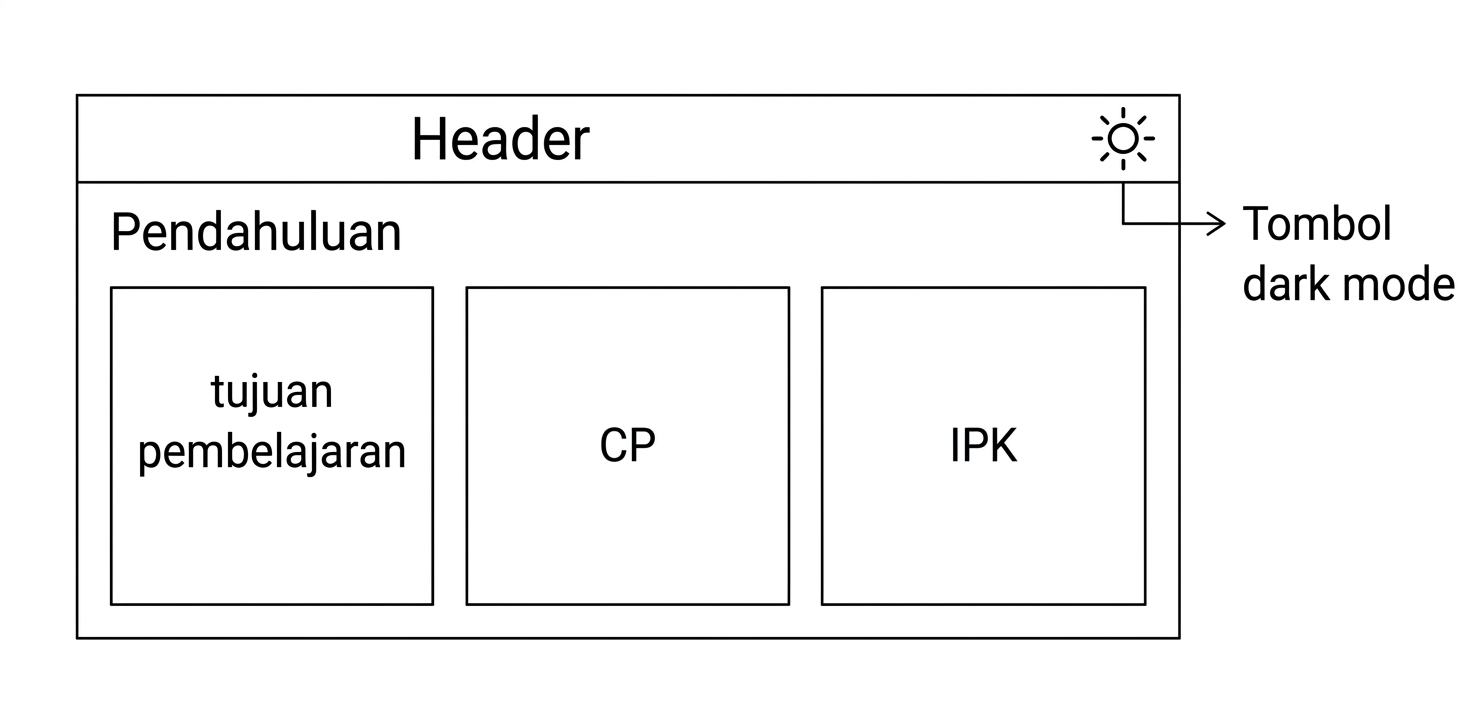
\includegraphics[width=0.8\textwidth]{images/pendahuluan2.png}
            \caption{Halaman Pendahuluan}
            \label{fig:pendahuluan}
        \end{figure}
        \begin{figure}[H]
            \centering
            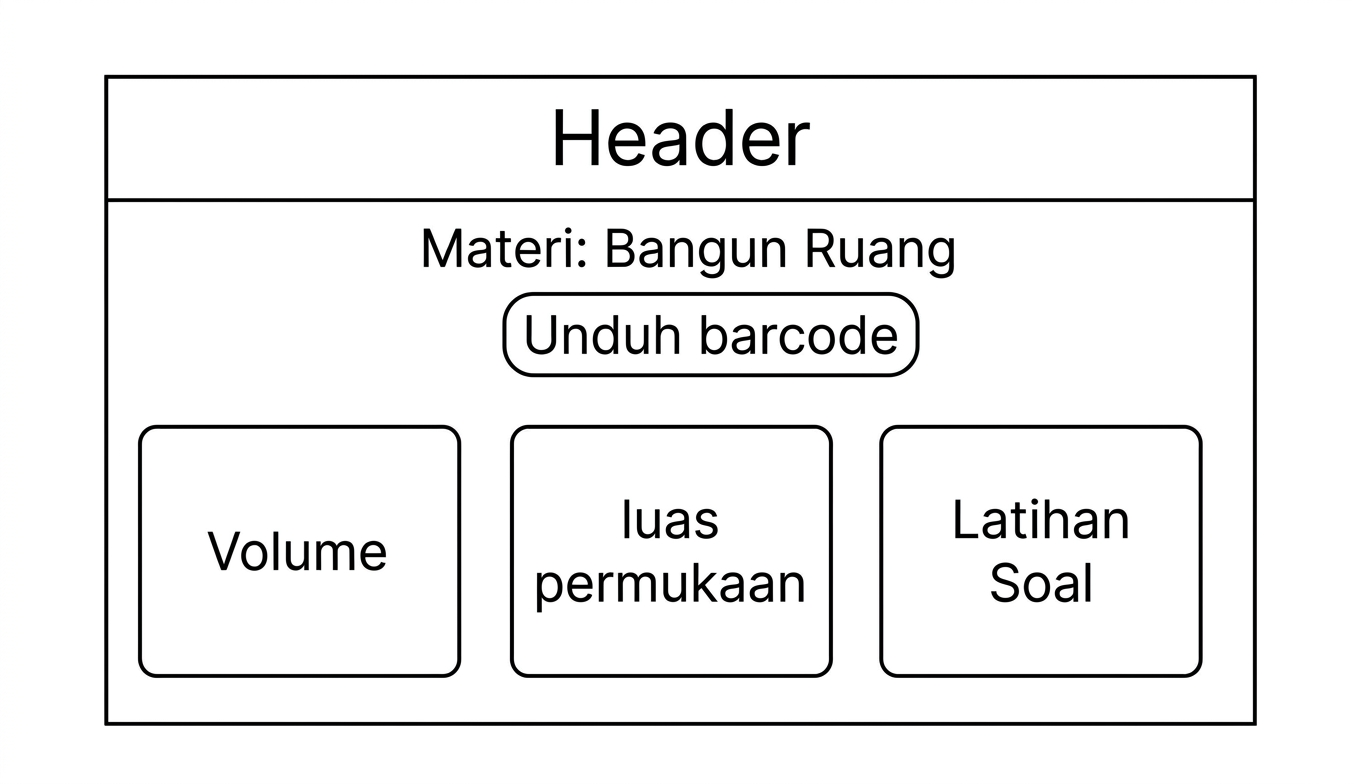
\includegraphics[width=0.8\textwidth]{images/menu2.png}
            \caption{Halaman Menu}
            \label{fig:halamanmenu}
        \end{figure}
        \begin{figure}[H]
            \centering
            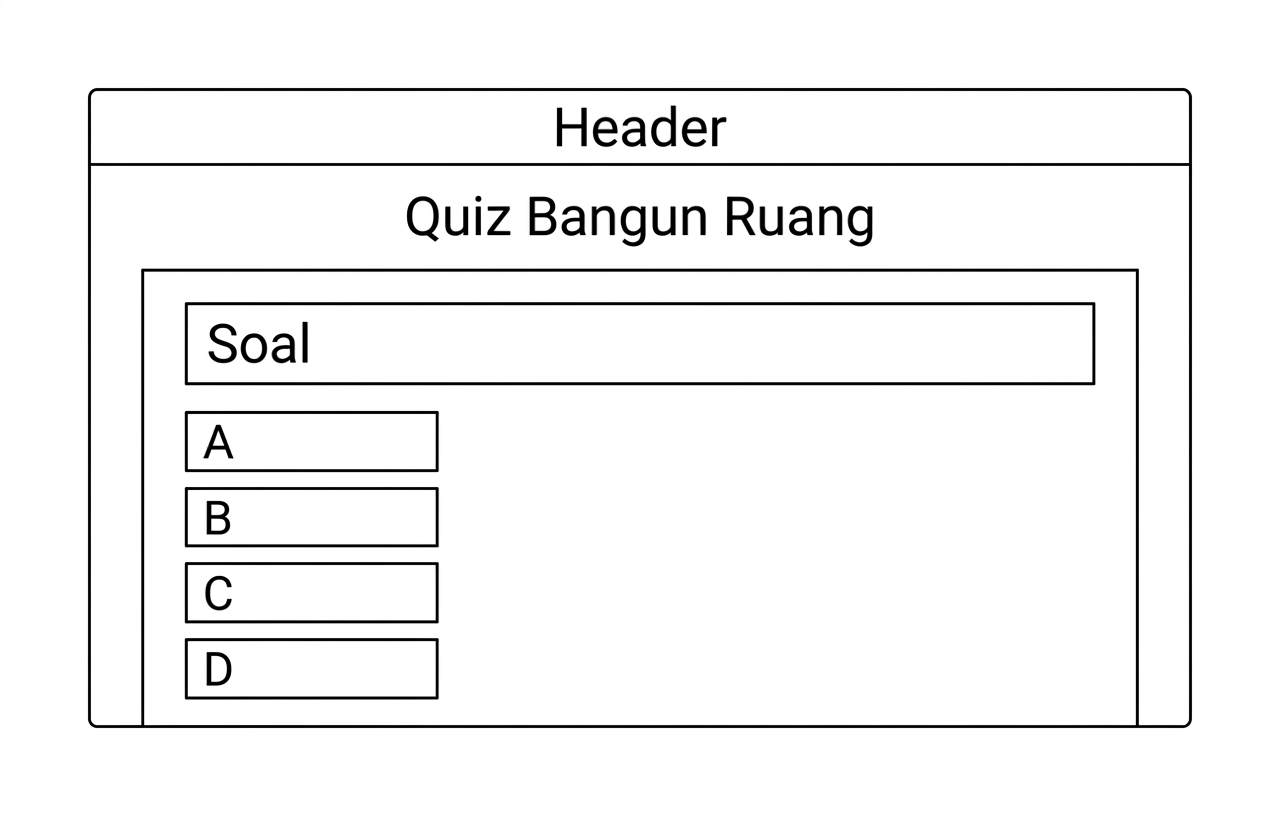
\includegraphics[width=0.8\textwidth]{images/quiz2.png}
            \caption{Halaman Quiz}
            \label{fig:halamanquiz}
        \end{figure}
        Selain merancang tampilan antarmuka pengguna (UI) melalui mockup, peneliti juga membuat diagram alur navigasi web untuk mengilustrasikan struktur dan aliran interaksi pengguna dalam sistem. Diagram alur navigasi ini dirancang untuk memastikan kemudahan navigasi dan pengalaman pengguna yang optimal. Berikut adalah rancangan alur navigasi yang telah dibuat:
        \begin{figure}[H]
            \centering
            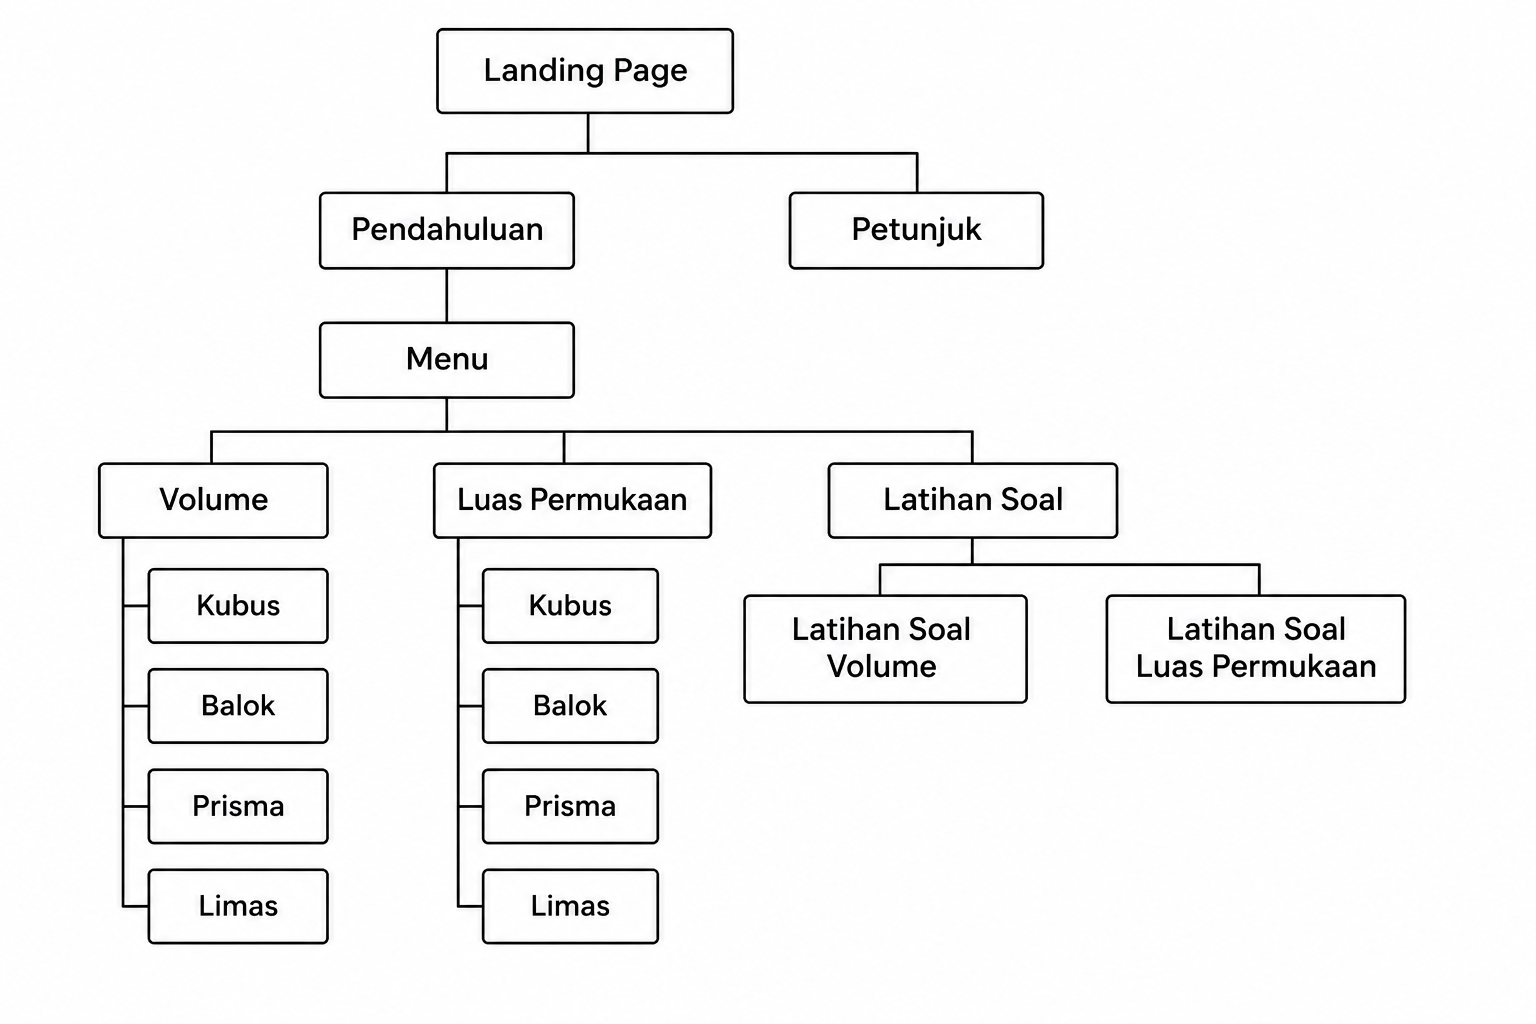
\includegraphics[width=0.8\textwidth]{images/Flow.png}
            \caption{Diagram Alur Navigasi Web}
            \label{fig:flowchart}
        \end{figure}
        \item Perancangan Interaksi Simulasi 3D
        \begin{figure}[H]
            \centering
            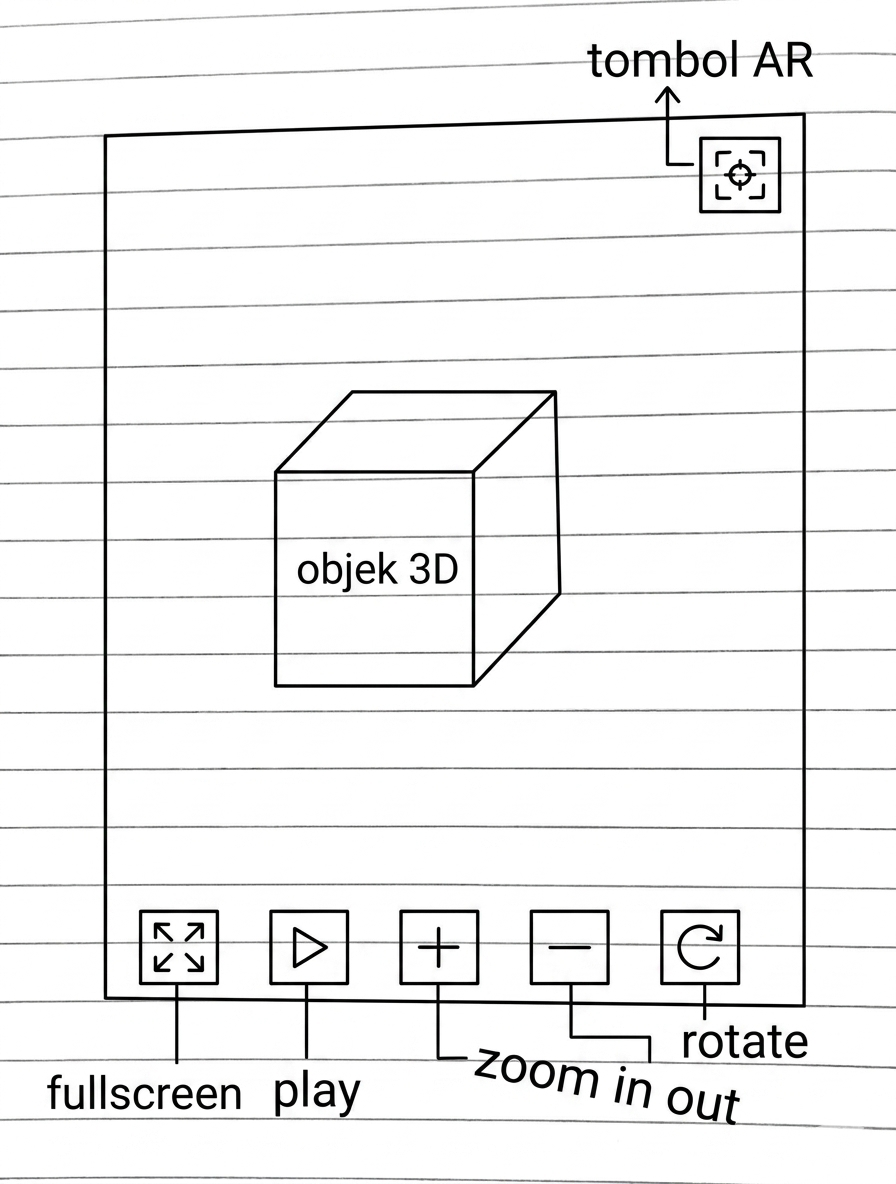
\includegraphics[width=0.5\textwidth]{images/mocksimulasi3d.png}
            \caption{Halaman Simulasi 3D}
            \label{fig:mocksimulasi3d}
        \end{figure}
        \hspace*{1cm}Desain antarmuka halaman simulasi 3D ditampilkan pada Gambar \ref{fig:mocksimulasi3d}. Pada tampilan tersebut terdapat objek 3D di tengah layar yang dapat dikendalikan melalui beberapa kontrol utama, antara lain:
        \begin{description}
            \item[Fullscreen:] Berpindah ke tampilan layar penuh untuk memperbesar area visualisasi.
            \item[Play / Pause:] Menjalankan atau menghentikan animasi objek 3D.
            \item[Zoom In / Zoom Out:] Memperbesar atau memperkecil tampilan objek untuk melihat detail atau konteks keseluruhan.
            \item[Rotate:] Memutar objek dengan kecepatan konstan; fitur ini dapat diaktifkan atau dinonaktifkan oleh pengguna.
            \item[AR:] Berpindah ke mode realitas tertambah (AR) menggunakan objek 3D yang sama. Untuk mode AR, objek 3D diekspor dan diunggah ke layanan mywebar.com sehingga dapat dimuat pada perangkat peserta didik.
        \end{description}
        \item Perancangan Objek 3D\\
        \hspace*{1cm}Objek 3D dibuat menggunakan perangkat lunak Blender. Objek yang dibuat meliputi kubus, balok, prisma, limas, serta jaring-jaring masing-masing bangun ruang. Semua objek diekspor dalam format .glb.
        \item Perancangan Arsitektur Web\\
        \hspace*{1cm}Arsitektur web dirancang sebagai aplikasi frontend berbasis \textbf{React.js} yang berperan sebagai Single Page Application (SPA). Pengembangan dilakukan secara lokal oleh tim pengembang menggunakan Node.js dan pengelola paket (npm atau yarn); seluruh kode sumber dikelola pada repositori GitHub. Struktur penyimpanan dan alur data dirancang sebagai berikut:

        \begin{enumerate}[leftmargin=*, label=--]
            \item Asset statis (gambar, berkas grafis) dan model 3D (format \texttt{.glb}) disimpan pada layanan Supabase Storage dan disajikan melalui URL publik atau CDN untuk akses cepat oleh klien.
            \item Komponen simulasi 3D diimplementasikan di sisi klien menggunakan Three.js di dalam komponen React, sehingga rendering dan interaksi (zoom, rotate, animasi) dijalankan di browser pengguna.
            \item Integrasi AR dilakukan dengan menyediakan model \texttt{.glb} pada layanan pihak ketiga (mis. mywebar.com) yang dapat memuat model dari Supabase; frontend memanggil URL AR saat mode AR diaktifkan.
            \item Variabel lingkungan sensitif (kunci API, URL storage) disimpan sebagai secret pada pengaturan Vercel dan tidak dikomit ke repositori.
            \item Continuous Deployment (CD): setiap perubahan yang dipush ke cabang utama pada GitHub memicu proses build otomatis di Vercel, yang meliputi instalasi dependensi, proses bundling React, dan penerapan ke domain produksi \textbf{https://medpemar.vercel.app}.
        \end{enumerate}

        \hspace*{1cm}Alur ini memastikan pemisahan tanggung jawab antara penyimpanan asset, logika aplikasi React, dan layanan AR eksternal. Diagram arsitektur sistem dan daftar teknologi yang digunakan disajikan pada Gambar \ref{fig:arsitekturweb}.
        \begin{figure}[H]
            \centering
            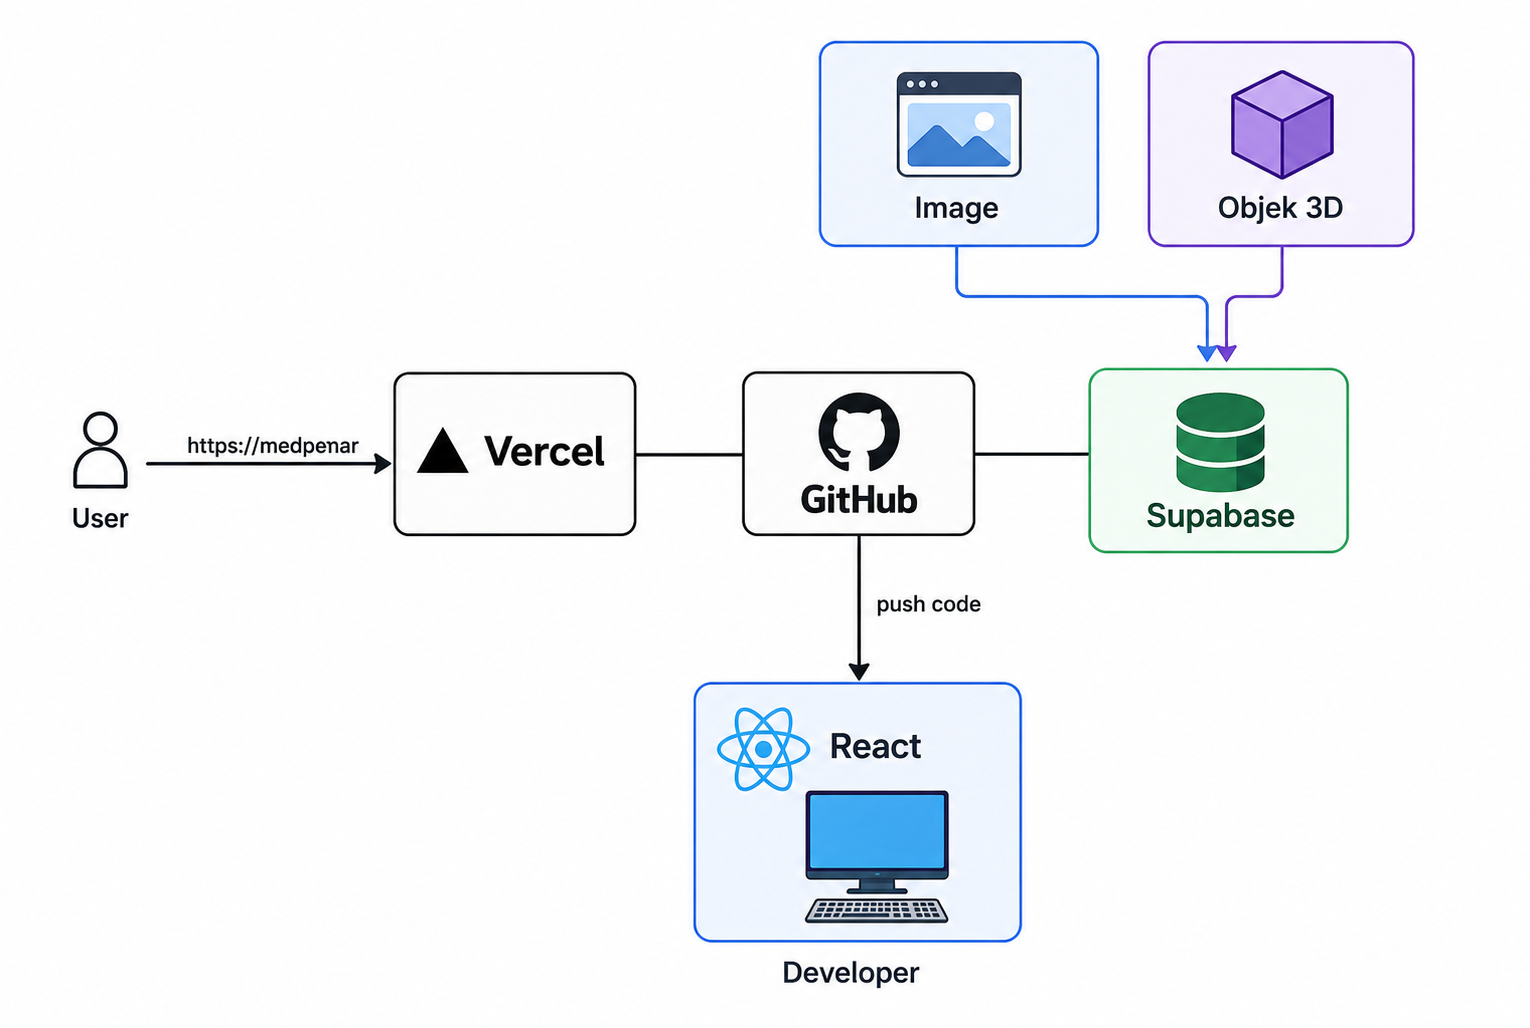
\includegraphics[width=1\textwidth]{images/Arsitektur.png}
            \caption{Arsitektur Web}
            \label{fig:arsitekturweb}
        \end{figure}

        

    \end{enumerate}

    \item \textbf{Pengembangan (Development)}\\
    \hspace*{1cm}Pengembangan media pembelajaran berbasis simulasi 3D tergolong kompleks. Teknologi simulasi 3D sendiri merupakan hal baru dalam dunia pendidikan, sehingga referensi untuk pengembangannya masih terbatas.
    Tahapan yang dilakukan peneliti dalam mengembangkan media pembelajaran berbasis simulasi 3D meliputi menyusun materi bangun ruang sisi datar, mendesain objek 3D bangun ruang menggunakan \textbf{Blender}, membuat desain grafis bangun datar dengan \textbf{GeoGebra}, serta membangun antarmuka aplikasi media pembelajaran berbasis web menggunakan \textbf{React JS}. 
    Berikut adalah penjabaran dari masing-masing tahapan tersebut.
    \begin{enumerate}[label=\arabic*)]
        \item Membuat Animasi 3D dengan Blender \\
        \hspace*{1cm}Pada materi bangun ruang sisi datar tentu terdapat objek bangun ruang seperti kubus, balok, prisma, dan limas. Peneliti membuat model bangun-bangun tersebut dengan bantuan aplikasi Blender, yang merupakan perangkat lunak untuk pembuatan objek 3D. Selain itu, Blender juga dapat digunakan untuk membuat animasi sederhana, misalnya animasi jaring-jaring bangun ruang agar materi lebih mudah dipahami oleh peserta didik. Desain 3D ini nantinya akan dijadikan objek dalam media pembelajaran berbasis simulasi 3D. Berikut contoh desain bangun ruang yang dibuat.
        \begin{figure}[H]
            \centering
            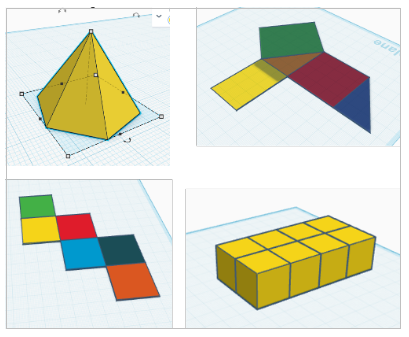
\includegraphics[width=0.4\textwidth]{images/bangun-dan-jaring.png}
            \caption{Desain 3D Bangun Ruang dan Jaring-jaring}
            \label{fig:bangundanjaring}
        \end{figure}
        \item Membuat Gambar Bangun Ruang dengan GeoGebra \\
        \hspace*{1cm}Gambar atau objek matematika yang terdapat dalam media ini sepenuhnya dibuat secara mandiri oleh peneliti. Objek-objek matematika, seperti persegi, kubus, balok, jaring-jaring, serta soal-soal, dibuat menggunakan aplikasi GeoGebra. Berikut ditampilkan contoh hasil pembuatannya.
        \begin{figure}[H]
            \centering
            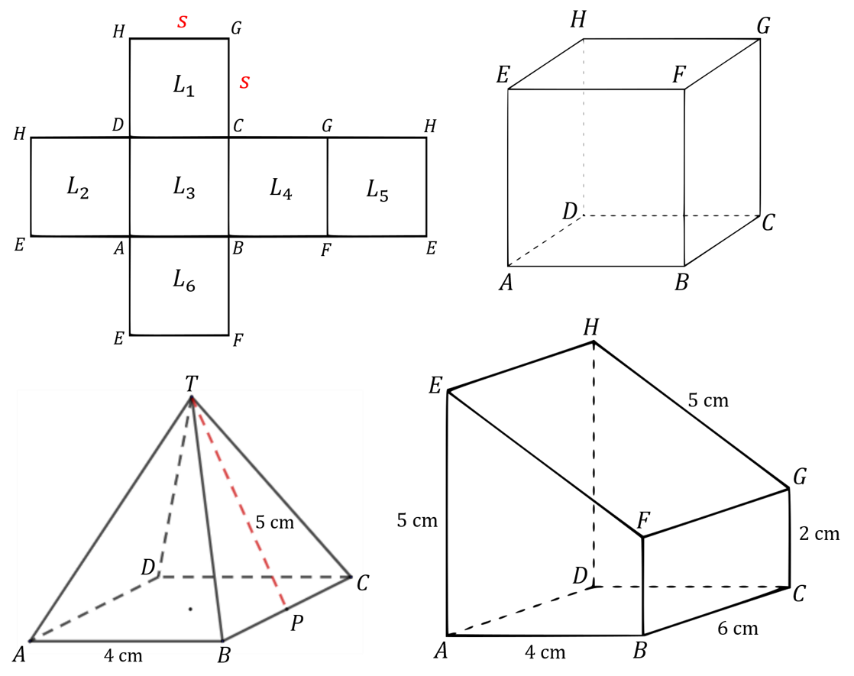
\includegraphics[width=0.4\textwidth]{images/hasil-geogebra.png}
            \caption{Desain 2D Bangun Ruang dan Jaring-jaring}
            \label{fig:hasilgeogebra}
        \end{figure}
        
        \item Membuat UI dengan React JS \\
        \hspace*{1cm}Agar media pembelajaran mudah diakses oleh peserta didik, peneliti membuat antarmuka menggunakan React JS. Antarmuka ini berbentuk situs web, sehingga peserta didik dapat dengan mudah mengakses media melalui domain yang diberikan. Untuk menampilkan simulasi 3D di situs web, peneliti menggunakan Three.js sebagai paket tambahan serta mywebar.com untuk menampilkan konten AR. Berikut ditampilkan contoh hasil pembuatannya.
        \begin{figure}[H]
            \centering
            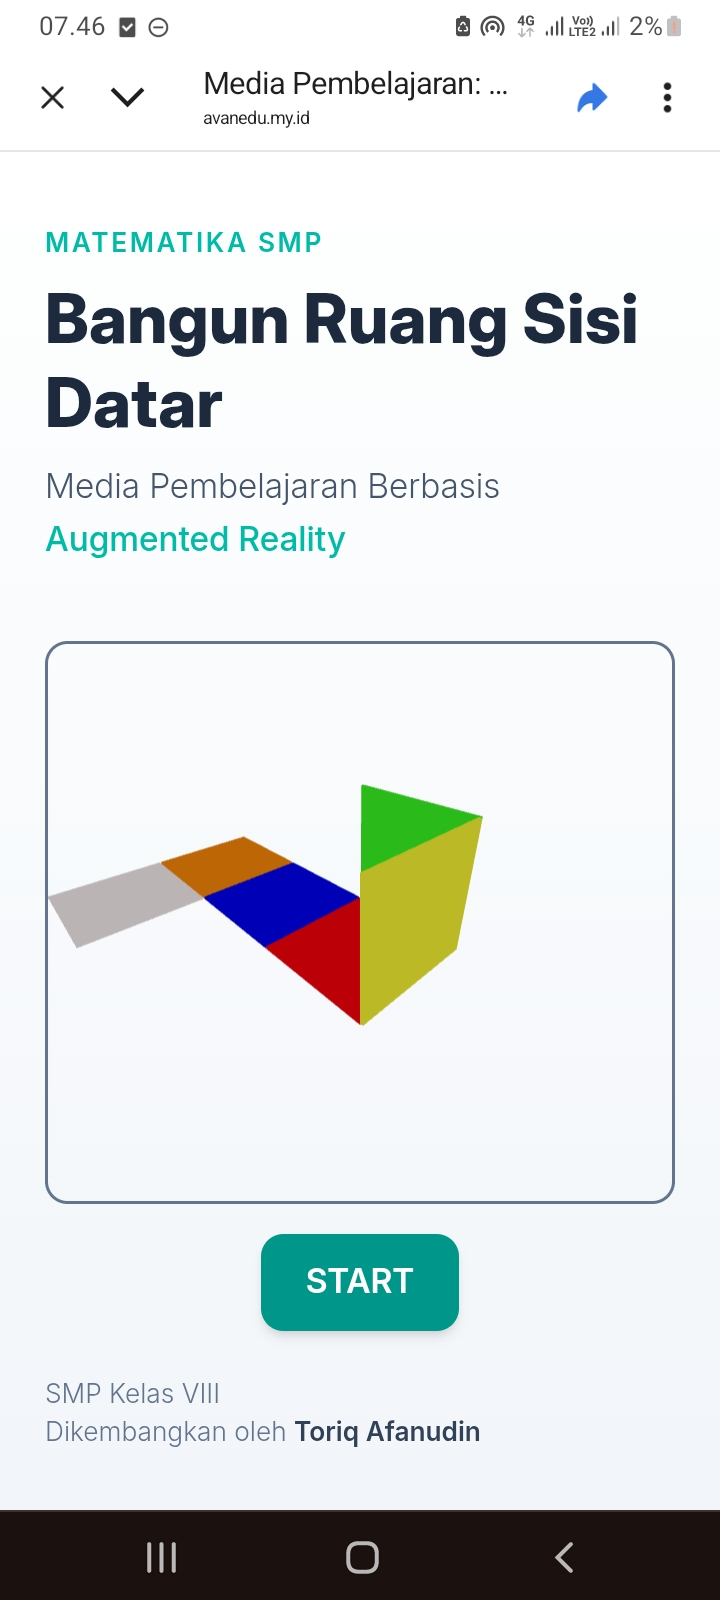
\includegraphics[width=0.3\textwidth]{images/ui-1.jpg}
            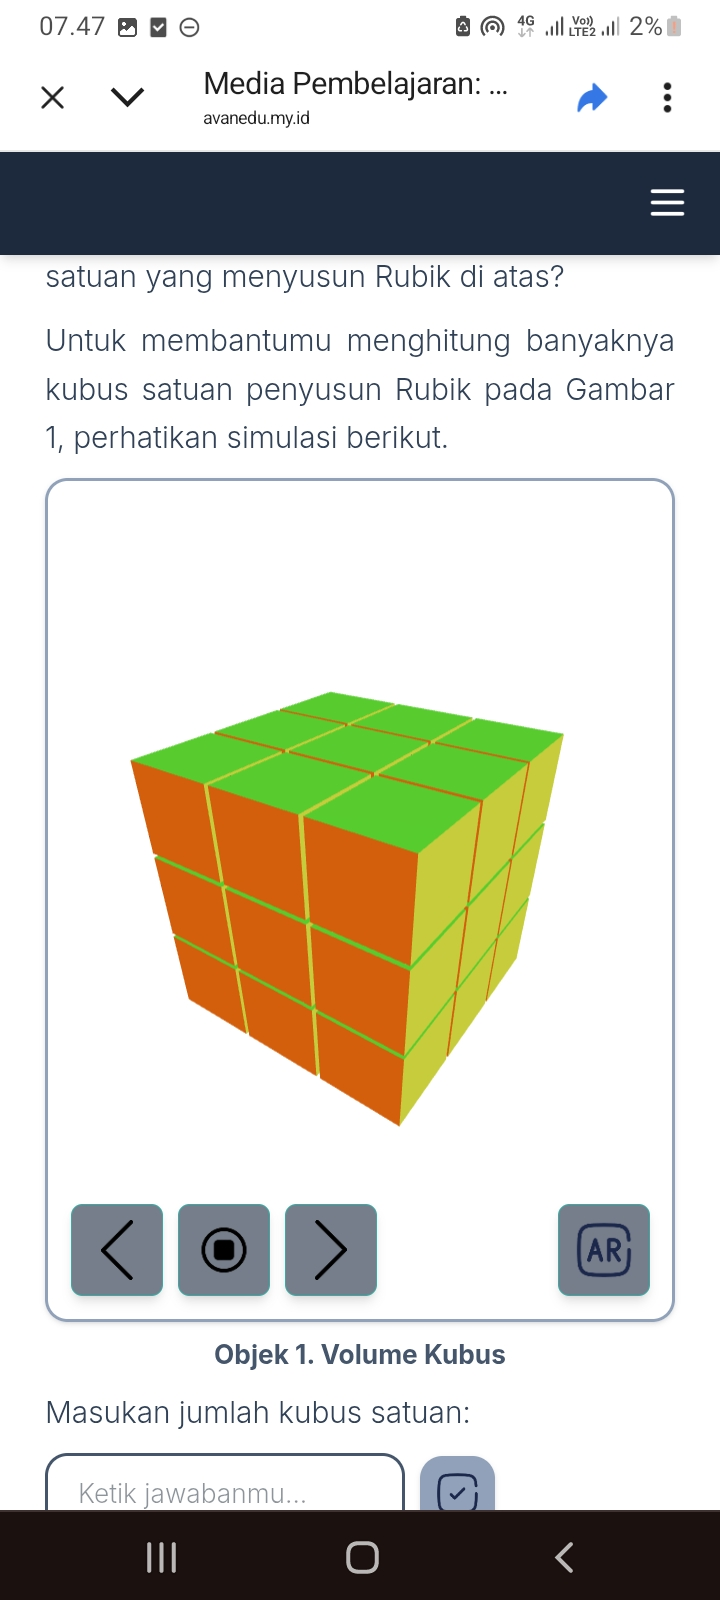
\includegraphics[width=0.3\textwidth]{images/ui-2.jpg}
            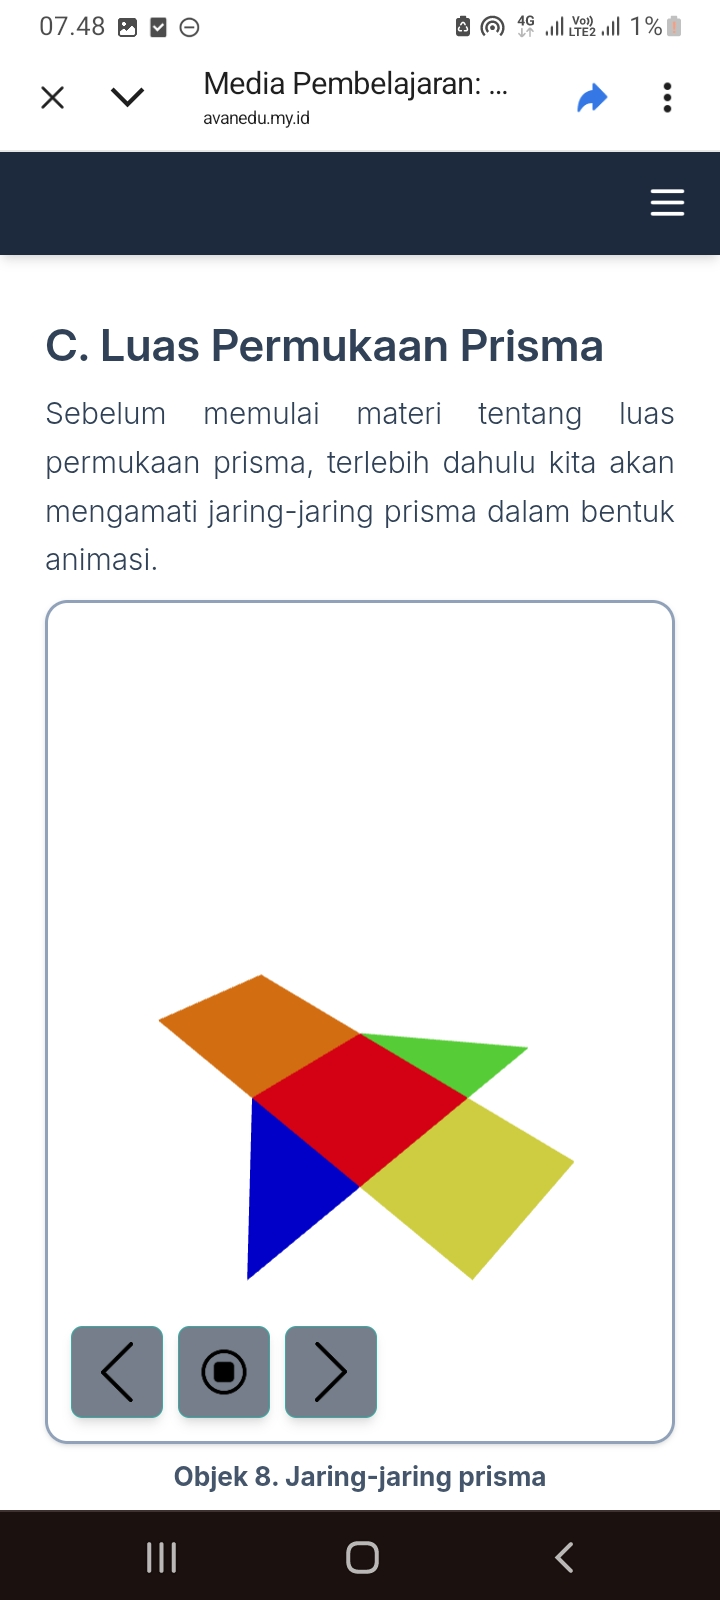
\includegraphics[width=0.3\textwidth]{images/ui-3.jpg}
            \caption{Antarmuka Media AR}
            \label{fig:antarmuka}
        \end{figure}

    \end{enumerate}

    \item \textbf{Implementasi}\\
    \hspace*{1cm}Pada tahap implementasi ini, peneliti melakukan uji coba terhadap produk yang telah dikembangkan. Uji coba dilakukan terhadap peserta didik kelas VIII-D SMP Muhammadiyah 9 Yogyakarta. Tahap ini bertujuan untuk memperoleh informasi mengenai kelayakan media pembelajaran yang telah dikembangkan. Pada tahap ini, terdapat dua jenis uji coba yang dilakukan, yaitu uji coba kelas kecil dan uji coba kelas besar. Berikut adalah penjelasan mengenai uji coba kelas kecil dan uji coba kelas besar.
    \begin{enumerate}
        \item Uji Coba Kelas Kecil \\
        \hspace*{1cm}Uji coba kelas kecil dilakukan dengan melibatkan beberapa peserta didik dari kelas VIII-D. Pelaksanaan uji coba ini dilakukan melalui kegiatan pembelajaran menggunakan media pembelajaran yang sedang dikembangkan. Setelah pembelajaran selesai, peserta didik diminta mengisi angket untuk memperoleh informasi mengenai respons mereka terhadap media tersebut. Uji coba kelas kecil dilaksanakan pada tanggal 14 Mei 2024 dengan melibatkan 7 peserta didik kelas VIII-D yang dipilih secara acak.

        \hspace*{1cm}Pada tahap awal uji coba kelas kecil, peneliti terlebih dahulu meminta izin kepada pendidik matematika untuk melaksanakan uji coba terhadap 7 peserta didik kelas VIII-D. Pemilihan peserta didik dilakukan secara acak oleh pendidik matematika kelas VIII-D. Uji coba dilakukan dengan memberikan media pembelajaran dan angket kepada peserta didik. Angket tersebut digunakan untuk memperoleh data penilaian peserta didik terhadap media pembelajaran yang sedang dikembangkan. Hasil dari penyebaran angket dapat dilihat pada Tabel 3.

        \item Uji Coba Kelas Besar \\
        \hspace*{1cm}Uji coba kelas besar dilakukan dengan melibatkan seluruh peserta didik kelas VIII-D SMP Muhammadiyah 9 Yogyakarta pada tanggal 16 Mei 2024. Pemilihan kelas tersebut didasarkan pada rekomendasi dari pendidik matematika. Alasan pemilihan ini adalah karena pendidik mengampu kelas tersebut dan peserta didik diketahui mengalami kesulitan dalam mempelajari materi bangun ruang.

        \hspace{1cm}Uji coba dilakukan melalui pembelajaran menggunakan media pembelajaran berbasis simulasi 3D. Setelah pembelajaran selesai, peserta didik diberikan angket. Angket tersebut digunakan untuk mengetahui penilaian peserta didik terhadap kualitas media pembelajaran yang dikembangkan. Pembelajaran dilaksanakan dengan membagi peserta didik ke dalam kelompok, disesuaikan dengan jumlah peserta didik yang membawa smartphone. Setelah peserta didik menyelesaikan materi dan soal-soal yang terdapat dalam media, mereka diminta untuk mengisi angket yang telah disediakan.
    \end{enumerate}

    \item \textbf{Evaluasi}
    
    \hspace{1cm}Tahap evaluasi merupakan tahap akhir dalam model pengembangan ADDIE. Evaluasi dilakukan untuk menganalisis hasil uji coba terhadap media pembelajaran berbasis simulasi 3D pada materi bangun ruang sisi datar kelas VIII. Tujuan dari tahap ini adalah untuk menyempurnakan produk yang telah dikembangkan sebelum menghasilkan produk akhir yang layak digunakan. Selanjutnya, dilakukan revisi akhir berdasarkan masukan dari ahli materi, ahli media, dan peserta didik.

    \hspace{1cm}Berdasarkan hasil validasi dari ahli materi dan ahli media, terdapat beberapa masukan terhadap media pembelajaran yang dikembangkan sebelum dilakukan uji coba kepada peserta didik. Selanjutnya, dilakukan revisi berdasarkan masukan tersebut hingga media pembelajaran masuk dalam kategori baik atau dinyatakan layak. Evaluasi yang dilakukan mencakup hasil validasi dari ahli materi dan ahli media, serta angket hasil uji coba media oleh peserta didik. Penilaian tersebut dijadikan acuan dalam menentukan kelayakan media pembelajaran yang dikembangkan.

\end{enumerate}
% ANALISIS DATA
\textbf{B. Analisis Data}
\addcontentsline{toc}{section}{B. Analisis Data}

\hspace{1cm}Analisis data merupakan tahap lanjutan dari tahap evaluasi dalam model pengembangan ADDIE. Data yang diperoleh dalam penelitian ini berupa data kualitatif yang kemudian dikonversi menjadi data kuantitatif. Analisis data dilakukan berdasarkan lembar penilaian dari ahli materi, ahli media, dan respons peserta didik. Media pembelajaran yang dikembangkan dinyatakan layak apabila memperoleh skor rata-rata penilaian dari ahli materi, ahli media, dan respons peserta didik minimal pada kategori "Baik". Berikut ini adalah hasil analisis data tersebut:
\begin{enumerate}
    \item Analisis Penilaian Angket Ahli Materi\\
    \hspace*{1cm}Validasi oleh ahli materi dilakukan untuk memperoleh penilaian berupa skor, komentar, dan masukan terhadap materi yang telah dikembangkan dalam media pembelajaran berbasis simulasi 3D. Komentar dan saran dari validator digunakan untuk menyempurnakan media pembelajaran agar menghasilkan produk akhir yang layak digunakan. Kelayakan materi dalam media pembelajaran ini dinilai oleh dua orang ahli, yaitu Ibu Rima Aksen Cahdriyana, M.Pd., dosen Pendidikan Matematika UAD sebagai validator 1, dan Bapak Wibowo Ramadhiyanto, S.Pd., pendidik Matematika di SMP Muhammadiyah 9 Yogyakarta, sebagai validator 2. Hasil penilaian kelayakan media pembelajaran disajikan pada Tabel \ref{penilaianmateri}.
    \begin{table}[H]
        \begin{adjustwidth}{-2cm}{-2cm}
            \centering
            \caption{Hasil Penilaian Materi Pembelajaran Berdasarkan Aspek Penilaian}
            \label{penilaianmateri}
            \begin{tabular}{|l|c|c|c|l|}
                \hline
                \textbf{Aspek} & \textbf{Validator 1} & \textbf{Validator 2} & \textbf{Rata-rata Skor} & \textbf{Kategori Kualitatif}\\
                \hline
                Aspek Isi & \(4\) & \(4{,}71\) & \(4{,}35\) & Sangat Baik\\
                Aspek Bahasa & \(4\) & 5 & \(4{,}5\) & Sangat Baik\\
                Aspek Penyajian & \(4{,}5\) & \(4{,}87\) & \(4{,}68\) & Sangat Baik\\
                Aspek Simulasi 3D & \(5\) & 5 & 5 & Sangat Baik\\
                \hline
                \multicolumn{3}{|c|}{Kesimpulan} & \(4{,}63\) & Sangat Baik\\
                \hline
            \end{tabular}
        \end{adjustwidth}
    \end{table}
    % \begin{table}[H]
    %     \begin{adjustwidth}{-2cm}{-2cm}
    %         \centering
    %         \caption{Hasil Penilaian Media Pembelajaran Menurut Ahli Media}
    %         \label{penilaianmateri}
    %         \begin{tabular}{|c|c|c|c|c|c|}
    %             \hline
    %             \textbf{No} & \textbf{Validator} & \textbf{Skor} & \textbf{Rata-rata Skor} & \textbf{Kriteria Data Kuantitatif}\\
    %             \hline
    %             1 & Rima Aksen Cahdriyana, M.Pd. & 0 & 0 & Sangat Baik\\
    %             2 & Wibowo Ramadhiyanto, S.Pd. & 0 & 0 & Sangat Baik\\
    %             \hline
    %             \multicolumn{2}{|c|}{Jumlah Skor} & 0 & & \\
    %             \hline
    %             \multicolumn{2}{|c|}{Rata-rata Keseluruhan} & 0 & 0 & Sangat Baik\\
    %             \hline
    %         \end{tabular}
    %     \end{adjustwidth}
    % \end{table}

    \begin{table}[H]
        \centering
        \caption{Kriteria Penilaian Ahli Materi dan Ahli Media}
        \begin{tabular}{|c|c|l|}
            \hline
            \textbf{No} & \textbf{Rentang Skor \( (i) \) Kuantitatif} & \textbf{Kategori Kualitatif}\\
            \hline
            1 & \( \bar{x} > 4{,}2 \) & Sangat Baik\\
            2 & \( 3{,}4 < \bar{x} \leq 4{,}2 \) & Baik\\
            3 & \( 2{,}6 < \bar{x} \leq 3{,}4 \) & Cukup Baik\\
            4 & \( 1{,}8 < \bar{x} \leq 2{,}6 \) & Kurang\\
            5 & \( \bar{x} \leq 1{,8} \) & Sangat Kurang\\
            \hline 
        \end{tabular}
    \end{table}
    \hspace*{1cm}Dari Tabel \ref{penilaianmateri} diperoleh skor rata-rata penilaian kedua validator sebesar \(4{,}63\). Mengacu pada kriteria penilaian yang ditetapkan pada Tabel \ref{kriteriaresponsiswa}, skor sebesar \(4{,}63\) berada di atas nilai ambang batas \(\bar{x} > 4{,}2\), sehingga termasuk dalam kategori \textbf{Sangat Baik}. Selain itu, kedua validator juga memberikan skor penuh sebesar 5 pada aspek simulasi 3D, yang menunjukkan bahwa penggunaan simulasi 3D dalam media pembelajaran mendapat respons yang sangat positif.

    \item Analisis Penilaian Angket Ahli Media\\
    \hspace*{1cm}Validasi oleh ahli media dilakukan untuk memperoleh penilaian berupa skor, komentar, dan masukan terhadap media pembelajaran yang dikembangkan. Komentar dan saran dari validator media digunakan untuk menyempurnakan media pembelajaran agar menghasilkan produk akhir yang layak digunakan. Kelayakan media pembelajaran ini dinilai oleh dua orang ahli media, yaitu Bapak Anggit Prabowo, M.Pd., dosen Pendidikan Matematika UAD sebagai validator 1, dan Bapak Wibowo Ramadhiyanto, S.Pd., pendidik Matematika di SMP Muhammadiyah 9 Yogyakarta sebagai validator 2. Hasil penilaian kelayakan oleh ahli media disajikan pada Tabel~\ref{penilaianmedia}.
    \begin{table}[H]
        \begin{adjustwidth}{-2cm}{-2cm}
            \centering
            \caption{Hasil Penilaian Media Pembelajaran Berdasarkan Aspek Penilaian}
            \label{penilaianmedia}
            \begin{tabular}{|l|c|c|c|l|}
                \hline
                \textbf{Aspek} & \textbf{Validator 1} & \textbf{Validator 2} & \textbf{Rata-rata Skor} & \textbf{Kategori Kualitatif}\\
                \hline
                Kualitas Kegrafikan & \(4{,}33\) & \(4{,}91\) & \(4{,}62\) & Sangat Baik\\
                Kelayakan Bahasa & \(4{,}33\) & \(4{,}75\) & \(4{,}54\) & Sangat Baik\\
                Kualitas Perangkat Lunak & \(4{,}66\) & \(5\) & \(4{,}83\) & Sangat Baik\\
                \hline
                \multicolumn{3}{|c|}{Kesimpulan} & \(4{,}66\) & Sangat Baik\\
                \hline
            \end{tabular}
        \end{adjustwidth}
    \end{table}

    % \begin{table}[H]
    %     \centering
    %     \caption{Kriteria Penilaian Ahli Media}
    %     \begin{tabular}{|c|c|c|}
    %         \hline
    %         \textbf{No} & \textbf{Rentang Skor \( (i) \) Kuantitatif} & \textbf{Kategori Kualitatif}\\
    %         \hline
    %         1 & \( \bar{x} > 4{,}21 \) & Sangat Baik\\
    %         2 & \( 3{,}41 < \bar{x} \leq 4{,}2 \) & Baik\\
    %         3 & \( 2{,}60 < \bar{x} \leq 3{,}41 \) & Cukup Baik\\
    %         4 & \( 1{,}80 < \bar{x} \leq 2{,}60 \) & Kurang\\
    %         5 & \( \bar{x} \leq 1{,80} \) & Sangat Kurang\\
    %         \hline 
    %     \end{tabular}
    % \end{table}
    \hspace*{1cm}Dari Tabel \ref{penilaianmedia} diperoleh skor rata-rata penilaian kedua validator sebesar \(4{,}66\). Mengacu pada kriteria penilaian yang ditetapkan pada Tabel \ref{kriteriaresponsiswa}, skor sebesar \(4{,}66\) berada di atas nilai ambang batas \(\bar{x} > 4{,}2\), sehingga termasuk dalam kategori \textbf{Sangat Baik}. Selain itu, kedua validator juga memberikan skor tinggi pada aspek kualitas perangkat lunak, dengan skor rata-rata sebesar \(4{,}83\), yang menunjukkan bahwa media pembelajaran berbasis simulasi 3D yang dikembangkan memiliki kualitas perangkat lunak yang sangat baik.

    \item Analisis Penilaian Angket Respons Peserta Didik\\
    \hspace*{1cm}Respons peserta didik diperoleh melalui uji coba kelas kecil dan uji coba kelas besar yang bertujuan untuk mendapatkan penilaian berupa skor, komentar, dan masukan terhadap media pembelajaran yang telah dikembangkan. Respons tersebut dianalisis berdasarkan hasil angket yang disebarkan kepada peserta didik kelas VIII-D SMP Muhammadiyah 9 Yogyakarta. Kriteria penilaian angket respons peserta didik disajikan pada Tabel \ref{kriteriaresponsiswa}. Kriteria ini mengacu pada buku Prof. Sugiyono 2019 tentang metode penelitian kuantitatif, kualitatif, dan R\&D. Adapun hasil uji coba kelas kecil disajikan pada Tabel~\ref{ujikelaskecil}.
    \begin{table}[H]
        \centering
        \caption{Kriteria Penilaian Respons Peserta Didik}
        \label{kriteriaresponsiswa}
        \begin{tabular}{|c|c|l|}
            \hline
            \textbf{No} & \textbf{Rentang Skor \( (i) \) Kuantitatif} & \textbf{Kategori Kualitatif}\\
            \hline
            1 & \( \bar{x} > 4{,}2 \) & Sangat Baik\\
            2 & \( 3{,}4 < \bar{x} \leq 4{,}2 \) & Baik\\
            3 & \( 2{,}6 < \bar{x} \leq 3{,}4 \) & Cukup Baik\\
            4 & \( 1{,}8 < \bar{x} \leq 2{,}6 \) & Kurang\\
            5 & \( \bar{x} \leq 1{,8} \) & Sangat Kurang\\
            \hline 
        \end{tabular}
    \end{table}
    \hspace*{1cm}Berdasarkan pengambilan data pada uji coba kelas kecil yang melibatkan lima orang peserta didik, diperoleh hasil sebagai berikut.
    \begin{table}[H]
        \centering
        \caption{Data Hasil Ujicoba Kelas Kecil}
        \label{ujikelaskecil}
        \begin{tabular}{|c|l|c|l|}
            \hline
            \textbf{No} & \textbf{Nama} & \textbf{Rata-rata Skor} & \textbf{Kategori Kualitatif} \\
            \hline
            1 & Gilang Affan A. & \(4{,}35\) & Sangat Baik \\
            2 & Rachma Riski & \(4{,}85\) & Sangat Baik \\
            3 & Alif Bagas P. & \(4{,}15\) & Baik \\
            4 & Jasmine Sekar C. A. & \(3{,}38\) & Cukup Baik \\
            5 & Meydita Maharani & \(4{,}85\) & Sangat Baik \\
            \hline
            \multicolumn{2}{|c|}{Rata-rata Kelas Kecil} & \(4{,}31\) & Sangat Baik \\
            \hline
        \end{tabular}
    \end{table}
    Hasil uji coba kelas kecil menunjukkan bahwa skor rata-rata respons peserta didik sebesar \(4{,}31\). Mengacu pada kriteria penilaian yang ditetapkan pada Tabel \ref{kriteriaresponsiswa}, skor sebesar \(4{,}31\) berada di atas nilai ambang batas \(\bar{x} > 4{,}2\), sehingga termasuk dalam kategori \textbf{Sangat Baik}. Peserta didik memberikan tanggapan bahwa media pembelajaran ini menarik, mudah dipahami, dan menyarankan untuk diterapkan pada materi pembelajaran lain. Dari hasil ini, tidak terdapat rekomendasi revisi yang signifikan untuk produk berdasarkan uji coba kelas kecil, sehingga bisa langsung dilanjutkan ke tahap uji coba kelas besar. 
    \begin{figure}[H]
        \centering
        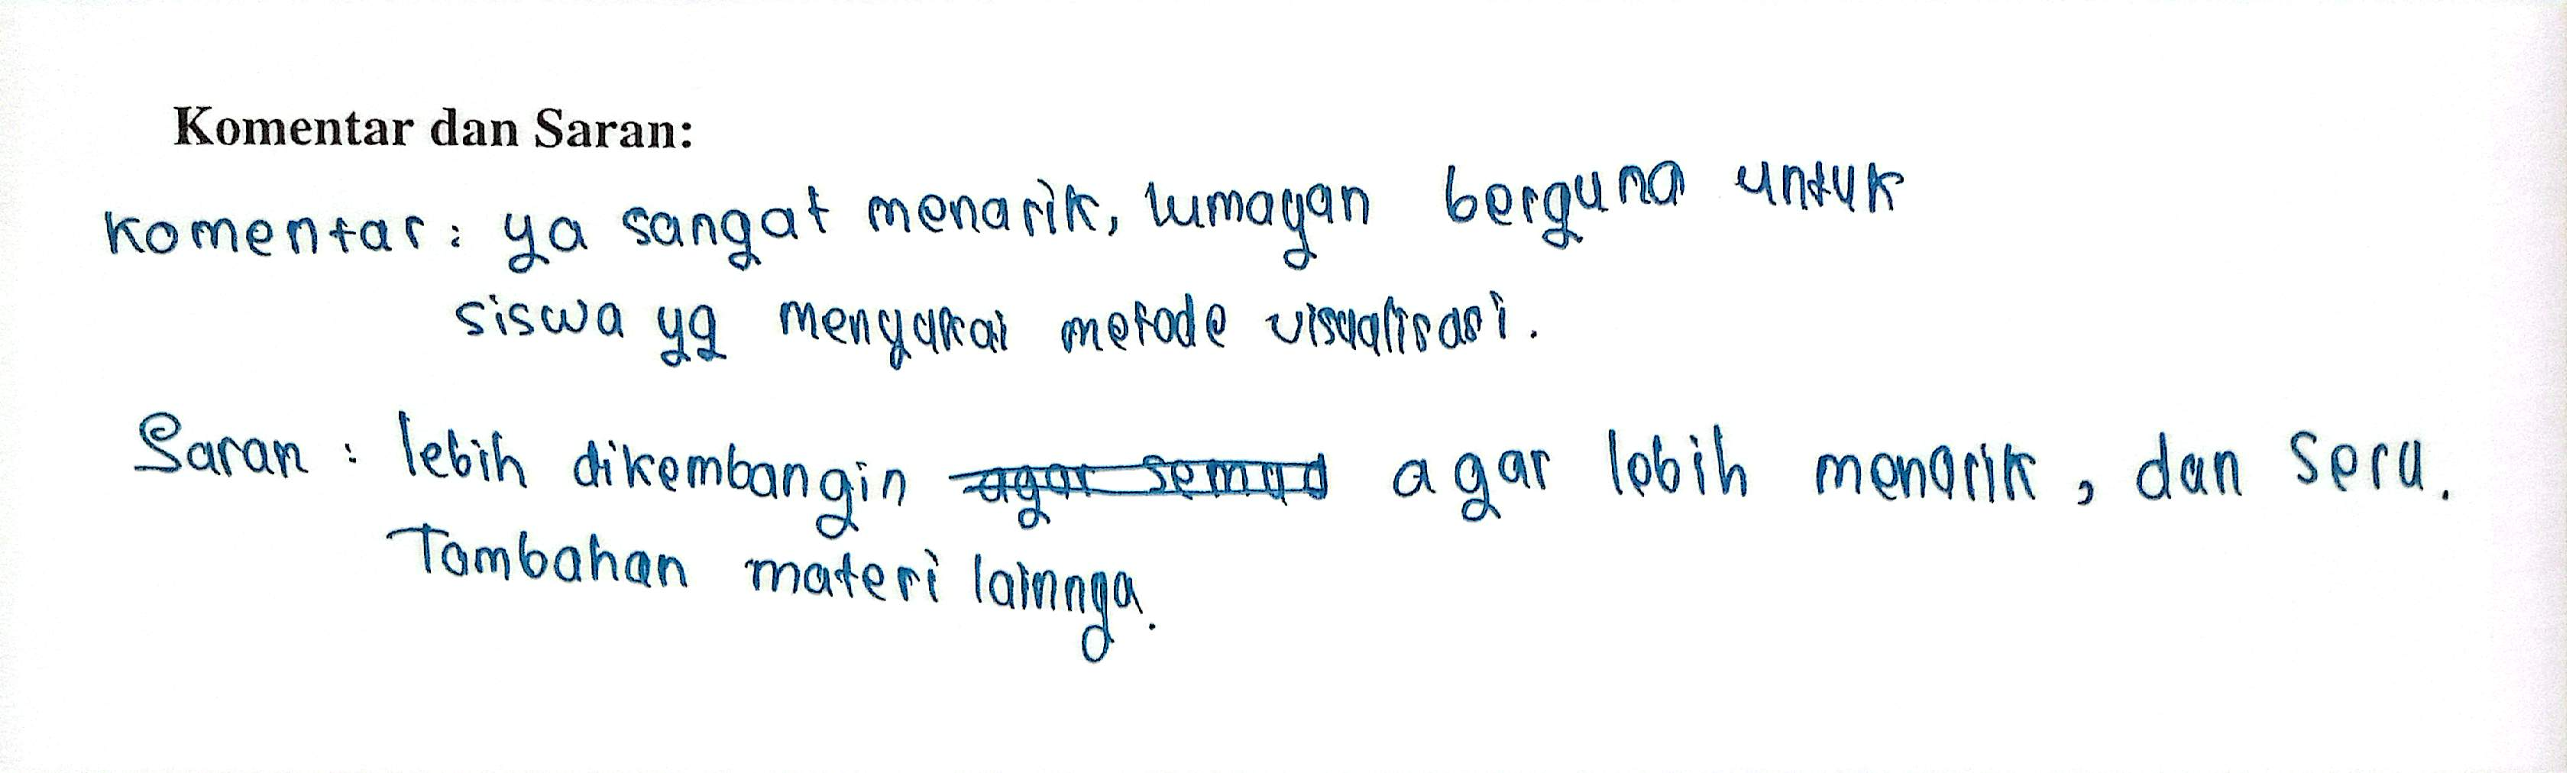
\includegraphics[width=1\textwidth]{komentar/kelaskecil1.jpg}
        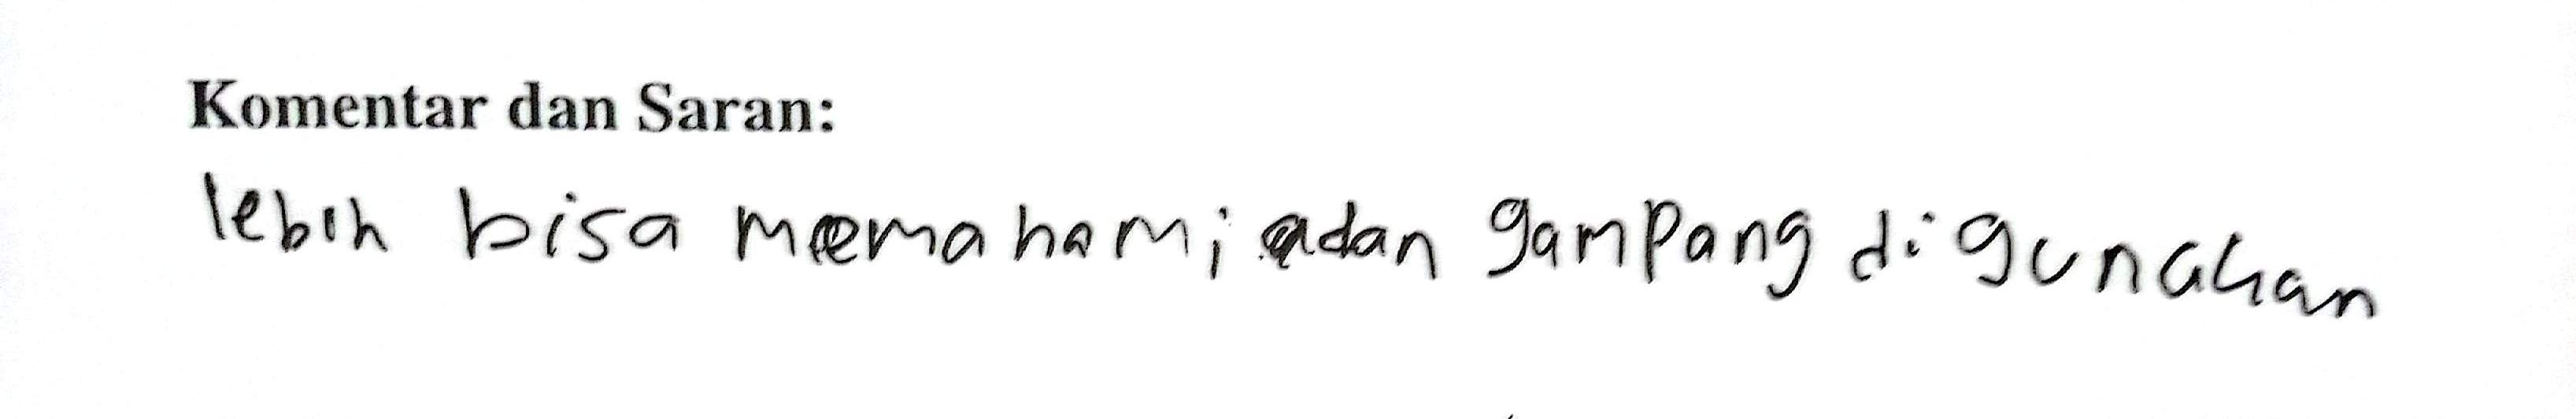
\includegraphics[width=1\textwidth]{komentar/kelaskecil2.jpg}
        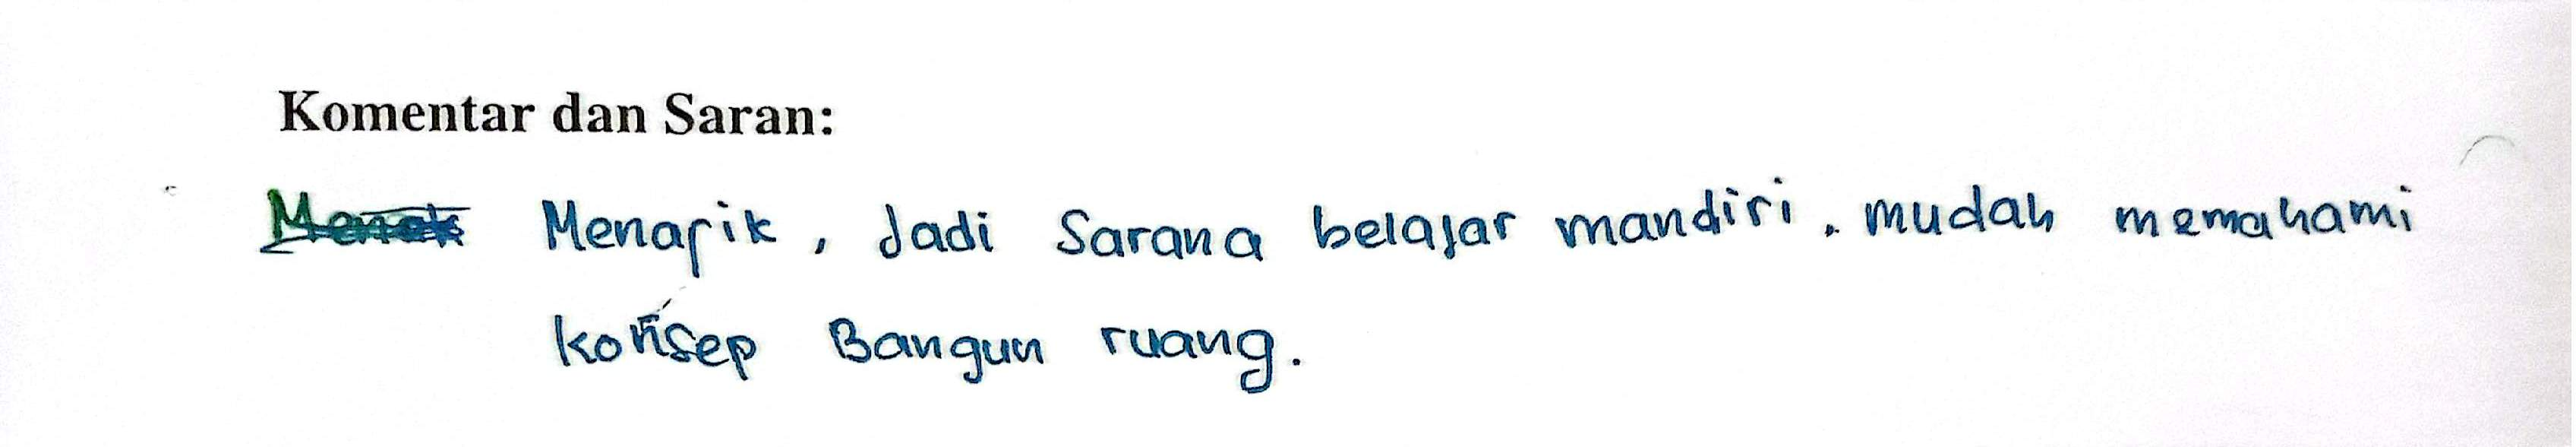
\includegraphics[width=1\textwidth]{komentar/kelaskecil3.jpg}
        \caption{Komentar dan Saran Kelas Kecil}
        \label{saran1}
    \end{figure}
    \hspace*{1cm}Berdasarkan pengambilan data pada uji coba kelas besar yang melibatkan 21 peserta didik kelas VIII-B, diperoleh hasil seperti pada Tabel \ref{ujikelasbesar}.
    \begin{table}[H]
        \centering
        \caption{Data Hasil Ujicoba Kelas Besar}
        \label{ujikelasbesar}
        \begin{tabular}{|c|l|c|l|}
            \hline
            \textbf{No} & \textbf{Nama} & \textbf{Rata-rata Skor} & \textbf{Kategori Kualitatif} \\
            \hline
            1 & Athayya Anindya & \(4{,}96\) & Sangat Baik \\
            2 & Dimas Galih M. & \(4{,}62\) & Sangat Baik \\
            3 & Arletta Prada R. & \(4{,}96\) & Sangat Baik \\
            4 & Sinayang Kusuma N. & \(4{,}96\) & Sangat Baik \\
            5 & Zahra Nurlinda & \(4{,}88\) & Sangat Baik \\
            6 & Faiza Putri & \(4{,}92\) & Sangat Baik \\
            7 & Arawinda Putri A. & \(4{,}88\) & Sangat Baik \\
            8 & Kaffa Naura Kanifda & \(4{,}08\) & Baik \\
            9 & Daffa Raqillarafa & \(4{,}15\) & Baik \\
            10 & Tri Rui & \(4{,}35\) & Sangat Baik \\
            11 & Sandika Saputra & \(4{,}77\) & Sangat Baik \\
            12 & Chyntia Azzahra A. & \(5\) & Sangat Baik \\
            13 & Itsya Rama M. & \(4{,}62\) & Sangat Baik \\
            14 & Ilham & \(4{,}35\) & Sangat Baik \\
            15 & Adinda Kamelia & \(4{,}19\) & Baik \\
            16 & Rafa Abiyu S. & \(4{,}65\) & Sangat Baik \\
            17 & Callysta & \(4{,}96\) & Sangat Baik \\
            18 & Vaneza Aullisya L. & \(4{,}04\) & Baik \\
            19 & M. Isakhan Amir & \(4{,}58\) & Sangat Baik \\
            20 & Ibrahim Putra M. & \(5\) & Sangat Baik \\
            21 & Daffa Prakoso & \(4{,}73\) & Sangat Baik \\
            \hline
            \multicolumn{2}{|c|}{Rata-rata Kelas Besar} & \(4{,}65\) & Sangat Baik \\
            \hline
        \end{tabular}
    \end{table}
    Hasil uji coba kelas besar menunjukkan bahwa skor rata-rata respons peserta didik sebesar \(4{,}65\). Mengacu pada kriteria penilaian yang ditetapkan pada Tabel \ref{kriteriaresponsiswa}, skor sebesar \(4{,}65\) berada di atas nilai ambang batas \(\bar{x} > 4{,}2\), sehingga termasuk dalam kategori \textbf{Sangat Baik}. Peserta didik memberikan umpan balik positif, meliputi pernyataan bahwa materi mudah dipahami, media pembelajaran menarik, dan simulasi 3D dapat meningkatkan motivasi belajar. Meskipun demikian, beberapa peserta didik memberikan rekomendasi untuk menambah jumlah contoh soal dengan tujuan meningkatkan pemahaman konsep. Dokumentasi lengkap dari komentar dan saran peserta didik tersaji secara rinci dalam lampiran penelitian ini.
    \item Kualitas Produk Secara Keseluruhan\\
    \hspace*{1cm}Kualitas media pembelajaran secara keseluruhan dinilai berdasarkan skor rata-rata dari ahli materi, ahli media, uji coba kelas kecil, dan uji coba kelas besar. Hasil perhitungan rata-rata keseluruhan dari keempat penilaian tersebut disajikan pada Tabel~\ref{ratakeseluruhan}.\\
    \begin{table}[H]
        \centering
        \caption{Hasil Rata-rata Keseluruhan}
        \label{ratakeseluruhan}
        \begin{tabular}{|c|l|c|l|}
            \hline
            \textbf{No} & \textbf{Sampel Uji Coba} & \textbf{Rata-rata} & \textbf{Kategori Kualitatif}\\
            \hline
            1 & Ahli Materi & \(4{,}63\) & Sangat Baik\\
            2 & Ahli Media & \( 4{,}66 \) & Sangat Baik\\
            3 & Uji Coba Kelas Kecil & \(4{,}31\) & Sangat Baik\\
            4 & Uji Coba Kelas Besar & \( 4{,}65 \) & Sangat Baik\\
            \hline
            \multicolumn{2}{|c|}{Rata-rata Keseluruhan} & \(4{,}56\) & Sangat Baik\\
            \hline
            
        \end{tabular}
    \end{table}
    \hspace*{1cm}Berdasarkan hasil perhitungan rata-rata keseluruhan pada Tabel~\ref{ratakeseluruhan}, diperoleh skor rata-rata sebesar \(4{,}56\). Mengacu pada kriteria penilaian yang telah ditetapkan pada Tabel \ref{kriteriaresponsiswa}, skor sebesar \(4{,}56\) berada di atas nilai ambang batas \(\bar{x} > 4{,}2\), sehingga termasuk dalam kategori \textbf{Sangat Baik}. Hasil ini menunjukkan bahwa media pembelajaran berbasis simulasi 3D yang dikembangkan memiliki kualitas yang sangat baik dan dinyatakan layak untuk digunakan dalam proses pembelajaran materi bangun ruang sisi datar untuk peserta didik kelas VIII.

\end{enumerate}
% REVISI PRODUK
\textbf{C. Revisi Produk}
\addcontentsline{toc}{section}{C. Revisi Produk}

\hspace*{1cm}Revisi produk merupakan langkah penting dalam pengembangan media pembelajaran. Revisi dilakukan apabila masih terdapat kesalahan atau kekurangan pada produk yang dikembangkan. Pada tahap ini, peneliti melakukan revisi terhadap media pembelajaran berdasarkan saran dan masukan dari ahli materi dan ahli media. Adapun proses revisi dalam pengembangan media pembelajaran ini adalah sebagai berikut:
\begin{enumerate}
    \item Revisi Produk Hasil Validasi Ahli Materi\\
    \hspace*{1cm}Berdasarkan masukan dari ahli materi, perbaikan yang dilakukan telah sesuai dengan saran dan rekomendasi yang diberikan. Ahli materi memberikan masukan terkait beberapa definisi dan kosakata yang perlu dirubah, agar lebih mudah dimengerti oleh peserta didik. Selain itu ahli materi juga meminta untuk ditambah page yang isinya adalah Capaian Kompetensi, Tujuan Pembelajaran, dan Indikator Pencapaian Kompetensi. Hasil perbaikan tersebut disajikan sebagai berikut.
    \begin{enumerate}
        \item Menambahkan kata "satuan" dalam kolom input jawaban kubus satuan.
        \begin{table}[H]
            \centering
            \begin{tabular}{c c}
                Sebelum Revisi & Sesudah Revisi \\
                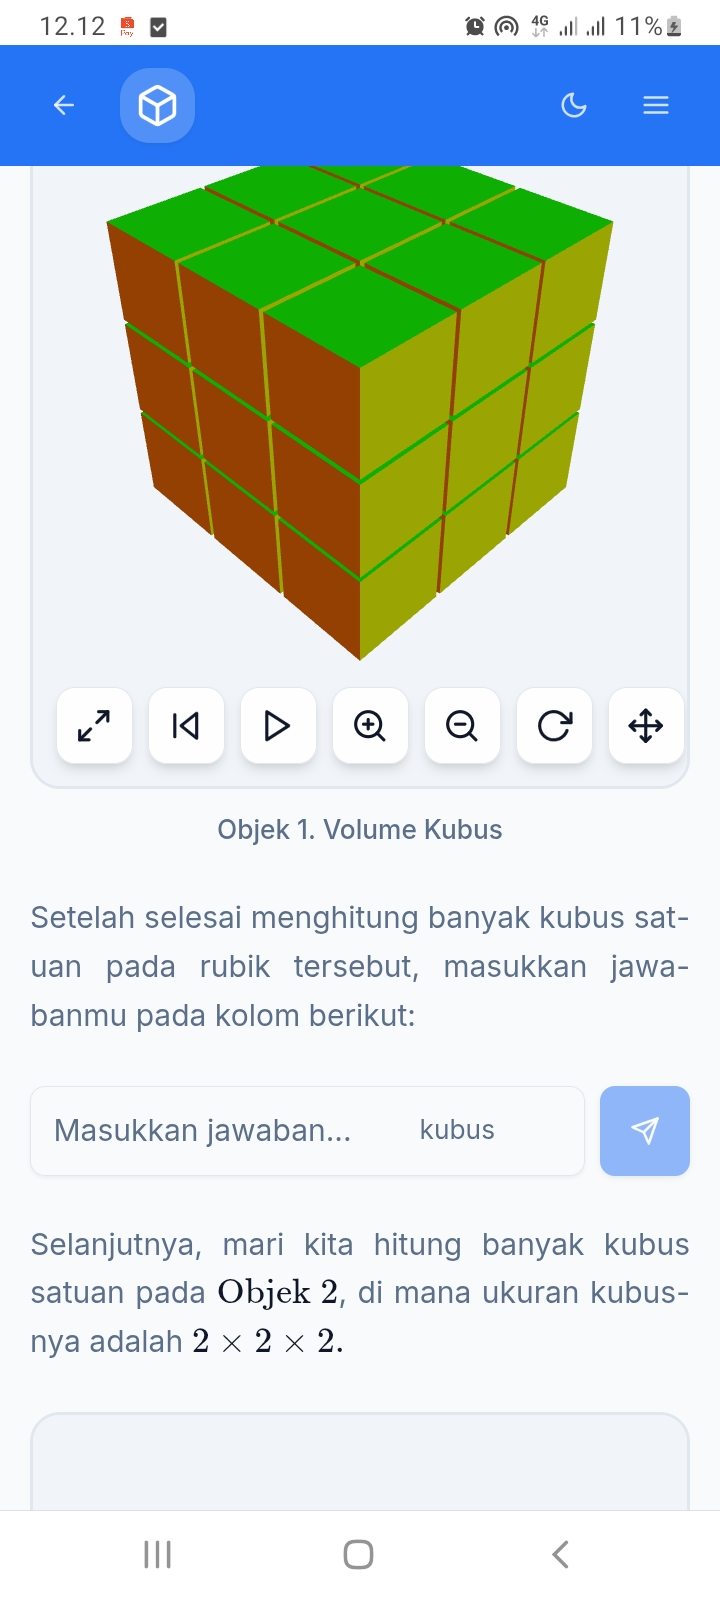
\includegraphics[width=0.25\textwidth]{revisi/sebelum/sebelumA.jpg} &
                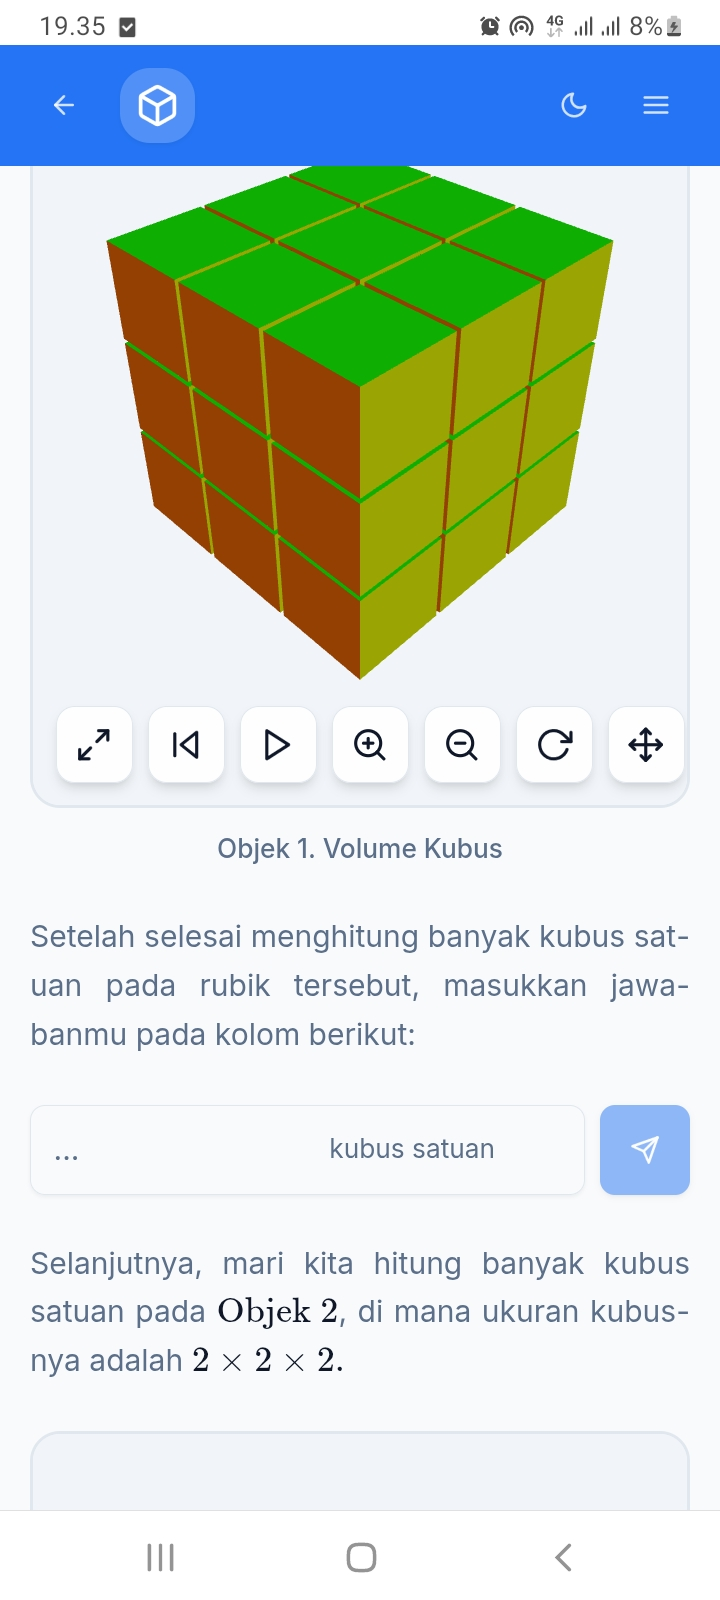
\includegraphics[width=0.25\textwidth]{revisi/sesudah/sesudahA.jpg} \\
            \end{tabular}
        \end{table}

        \item Memperbaiki definisi kubus yang kubus satuannya tidak ditampilkan.
        \begin{table}[H]
            \centering
            \begin{tabular}{c c}
                Sebelum Revisi & Sesudah Revisi \\
                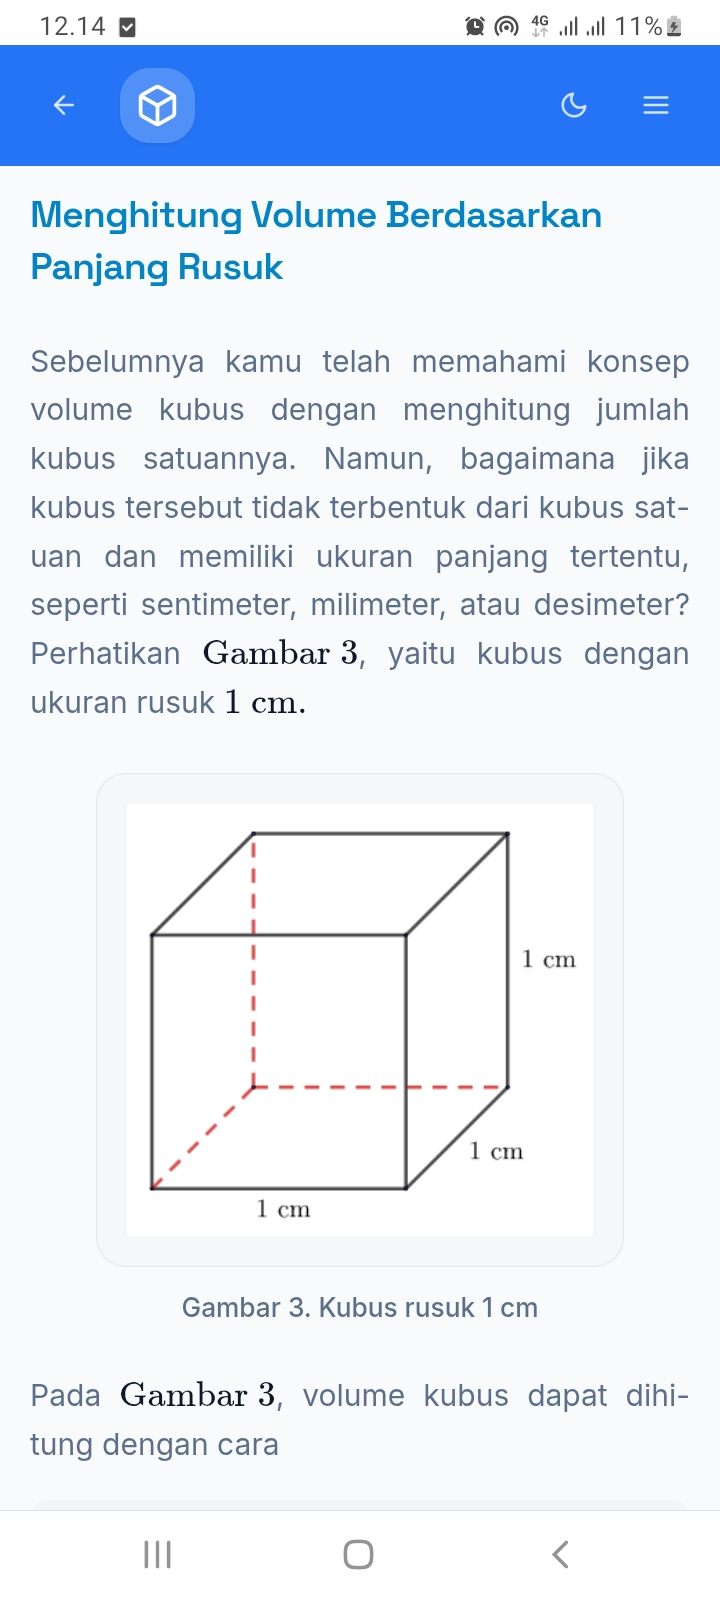
\includegraphics[width=0.25\textwidth]{revisi/sebelum/sebelumB.jpg} &
                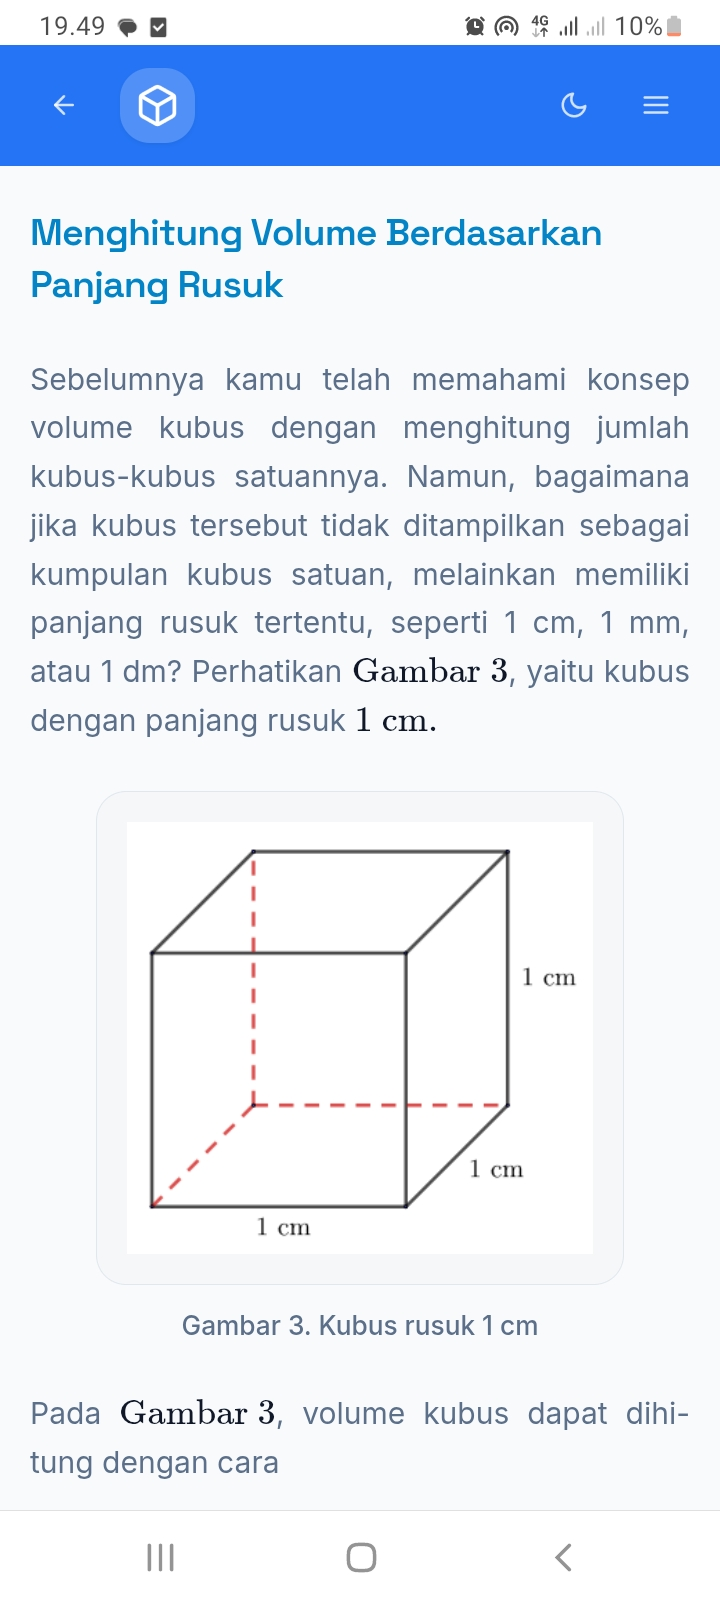
\includegraphics[width=0.25\textwidth]{revisi/sesudah/sesudahB.jpg} \\
            \end{tabular}
        \end{table}
        \item Mengganti kata "representasi" dengan kalimat yang mudah dipahami siswa SMP.
        \begin{table}[H]
            \centering
            \begin{tabular}{c c}
                Sebelum Revisi & Sesudah Revisi \\
                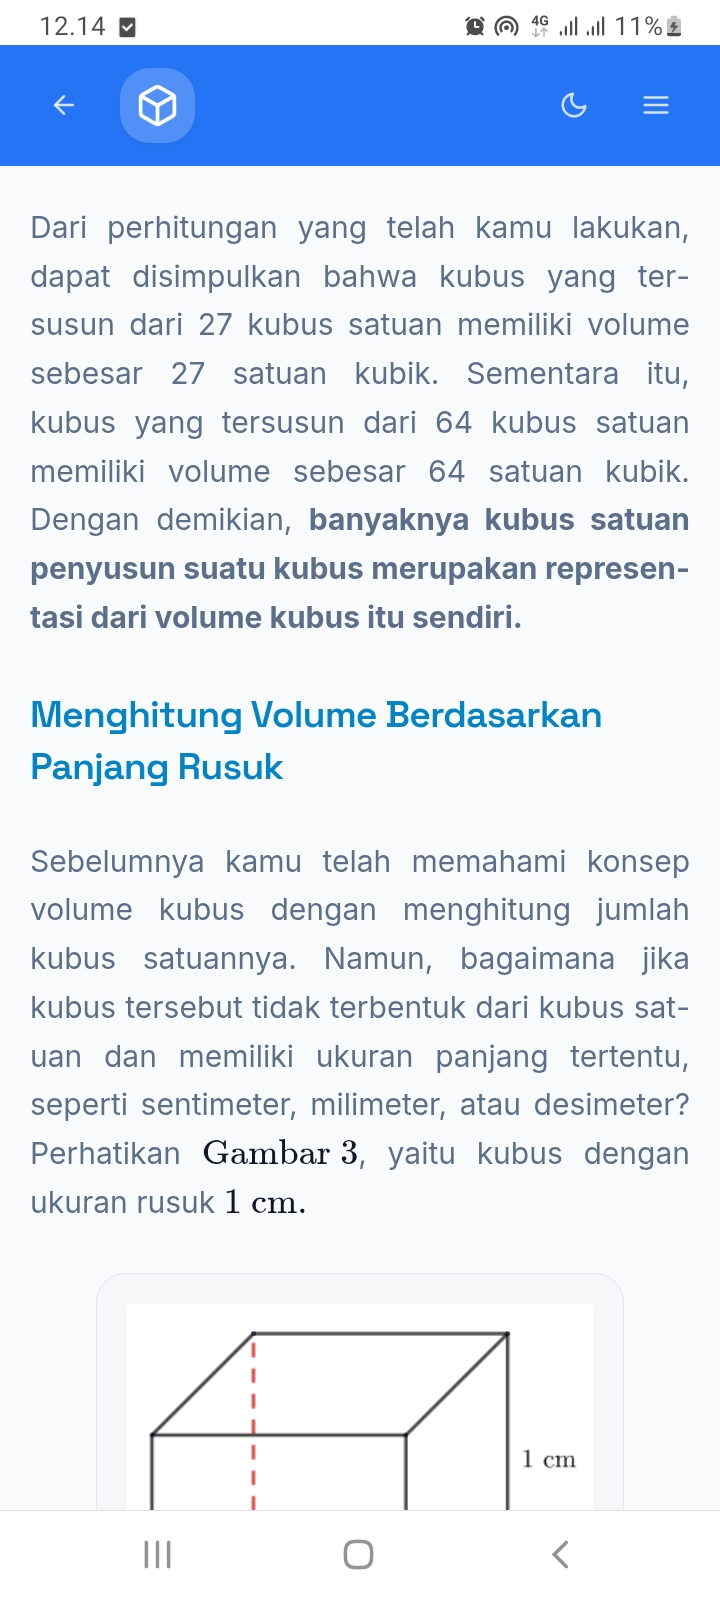
\includegraphics[width=0.25\textwidth]{revisi/sebelum/sebelumC.jpg} &
                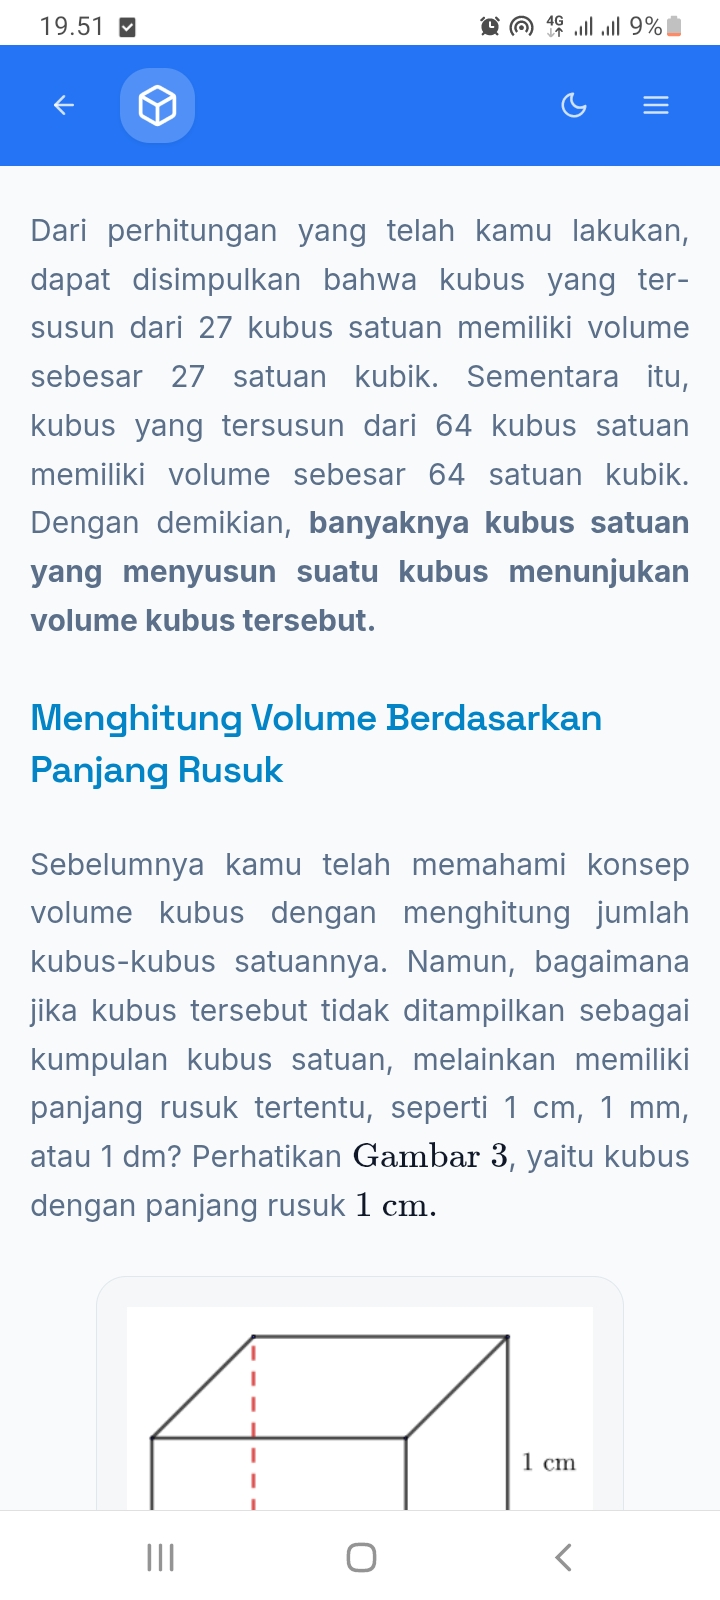
\includegraphics[width=0.25\textwidth]{revisi/sesudah/sesudahC.jpg} \\
            \end{tabular}
        \end{table}
        \item Memperbaiki definisi prisma agar tidak membingungkan siswa.
        \begin{table}[H]
            \centering
            \begin{tabular}{c c}
                Sebelum Revisi & Sesudah Revisi \\
                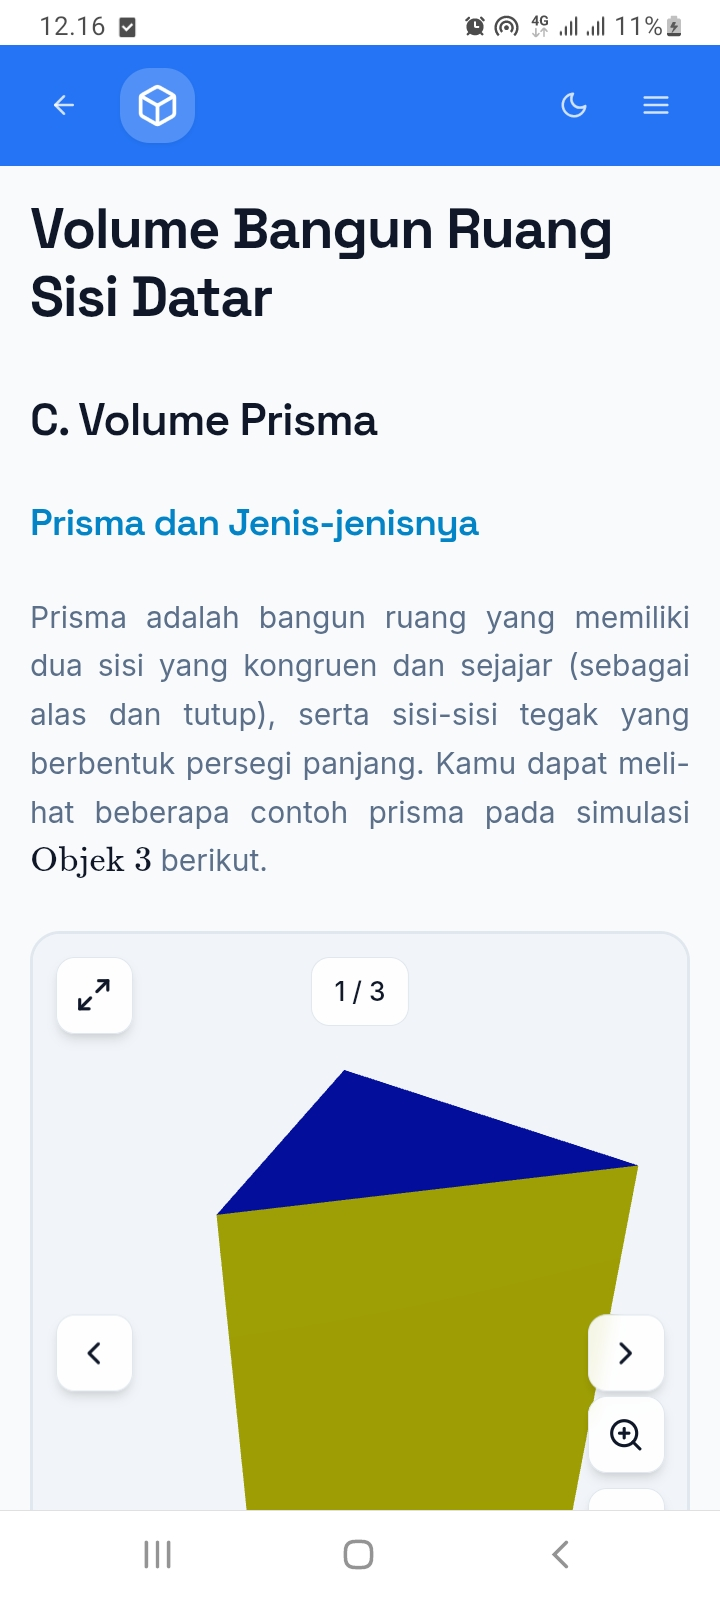
\includegraphics[width=0.25\textwidth]{revisi/sebelum/sebelumD.jpg} &
                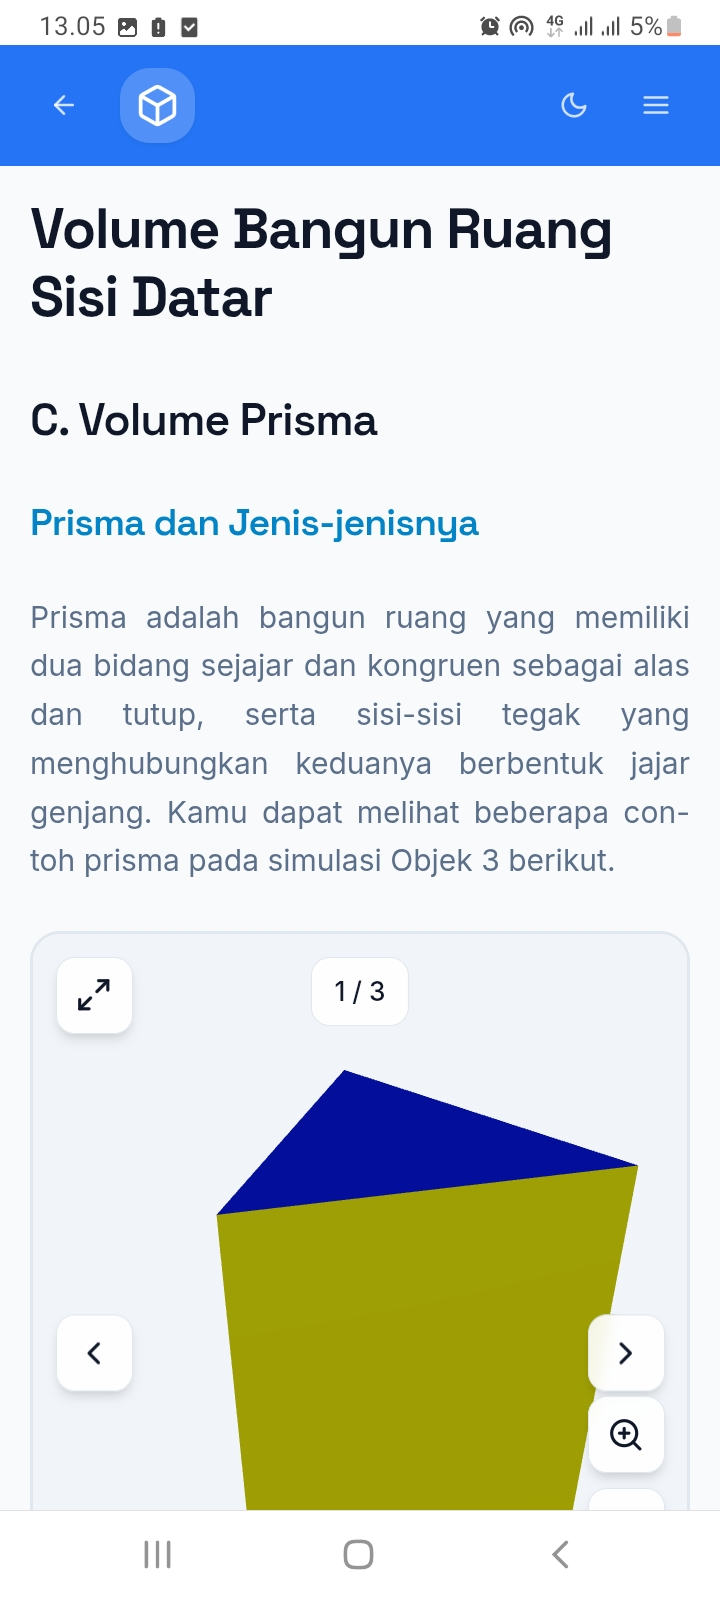
\includegraphics[width=0.25\textwidth]{revisi/sesudah/sesudahD.jpg} \\
            \end{tabular}
        \end{table}
        \item Menambahkan satu paragraf sebelum definisi jaring-jaring.
        \begin{table}[H]
            \centering
            \begin{tabular}{c c}
                Sebelum Revisi & Sesudah Revisi \\
                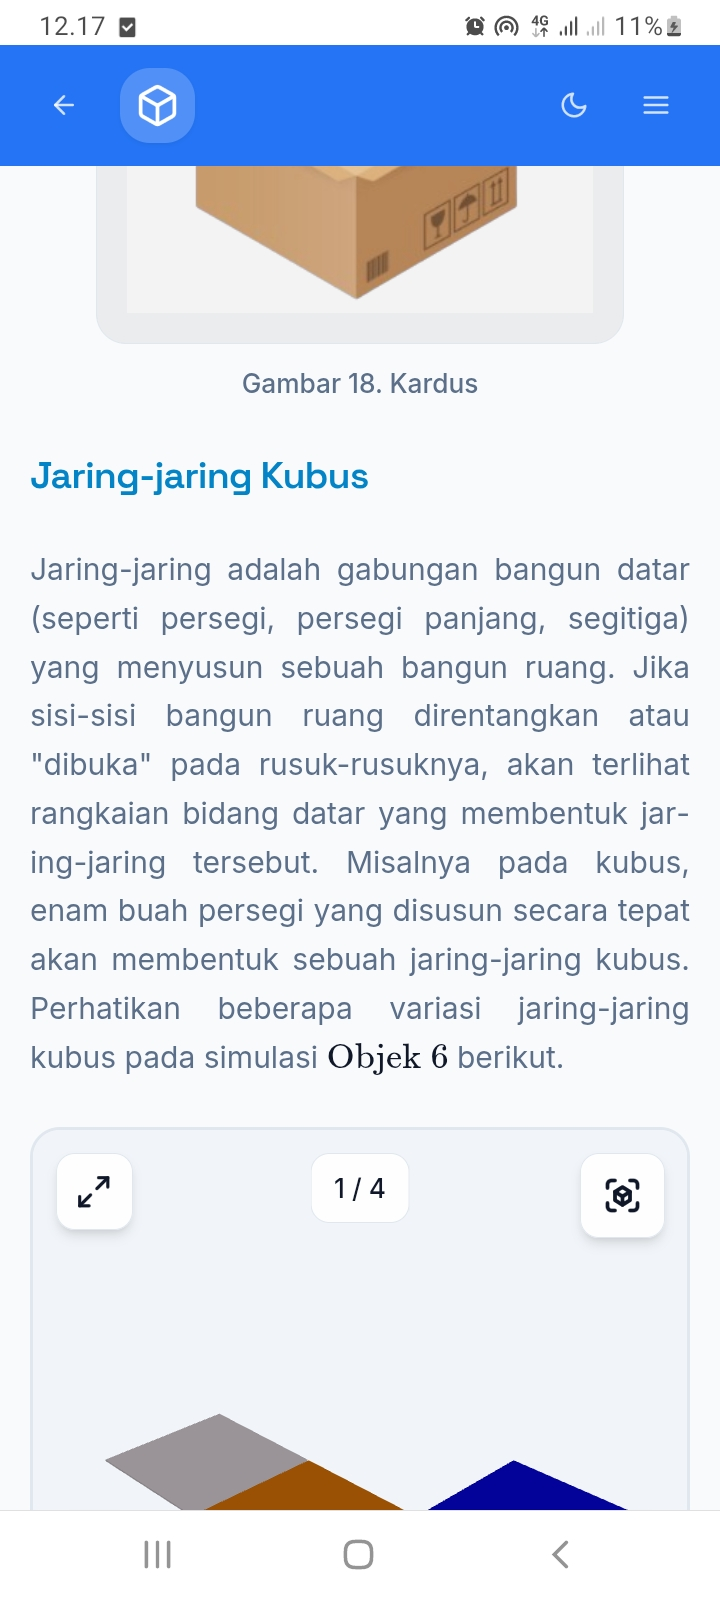
\includegraphics[width=0.25\textwidth]{revisi/sebelum/sebelumE.jpg} &
                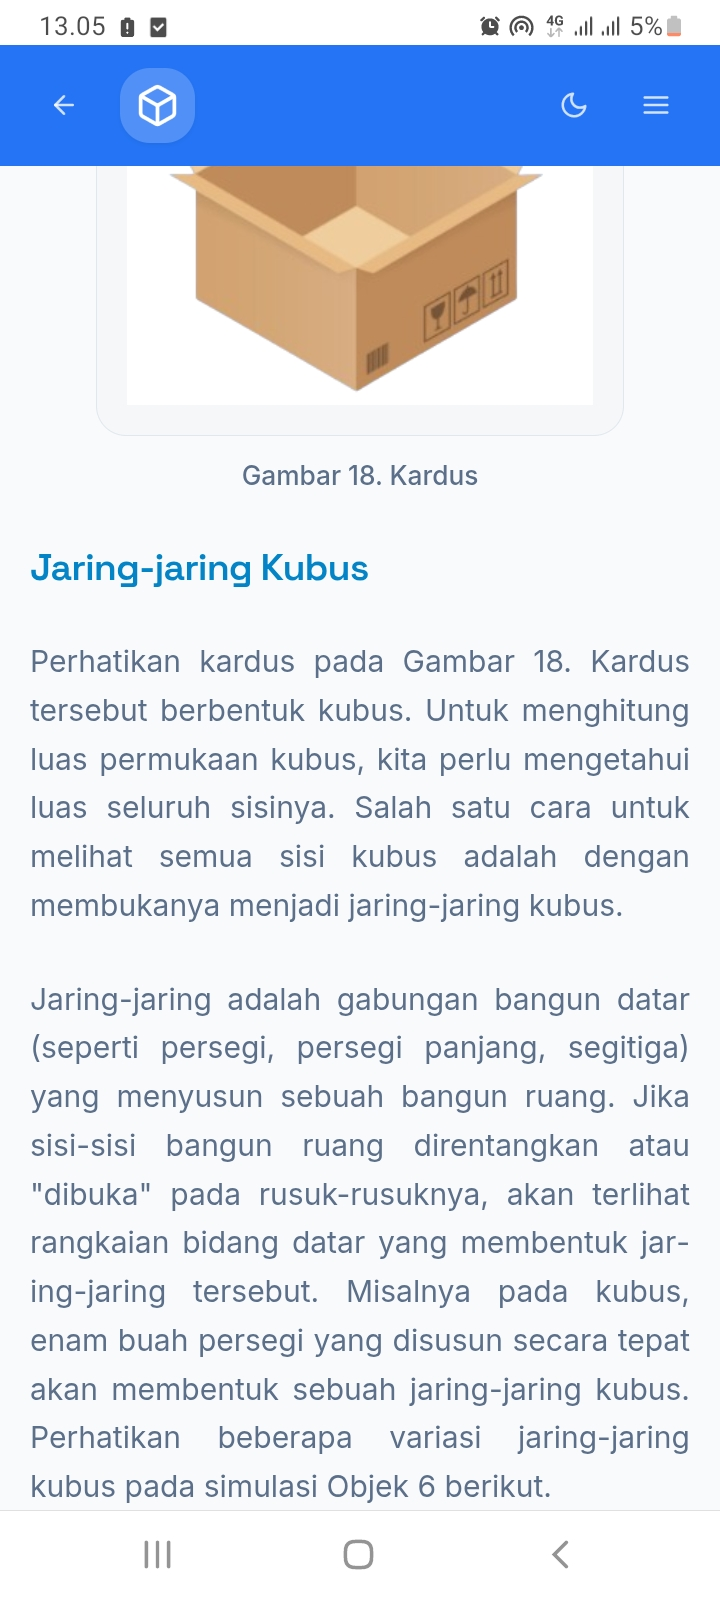
\includegraphics[width=0.25\textwidth]{revisi/sesudah/sesudahE.jpg} \\
            \end{tabular}
        \end{table}
        \item Menambah variasi jaring-jaring prisma.
        \begin{table}[H]
            \centering
            \begin{tabular}{c c}
                Sebelum Revisi & Sesudah Revisi \\
                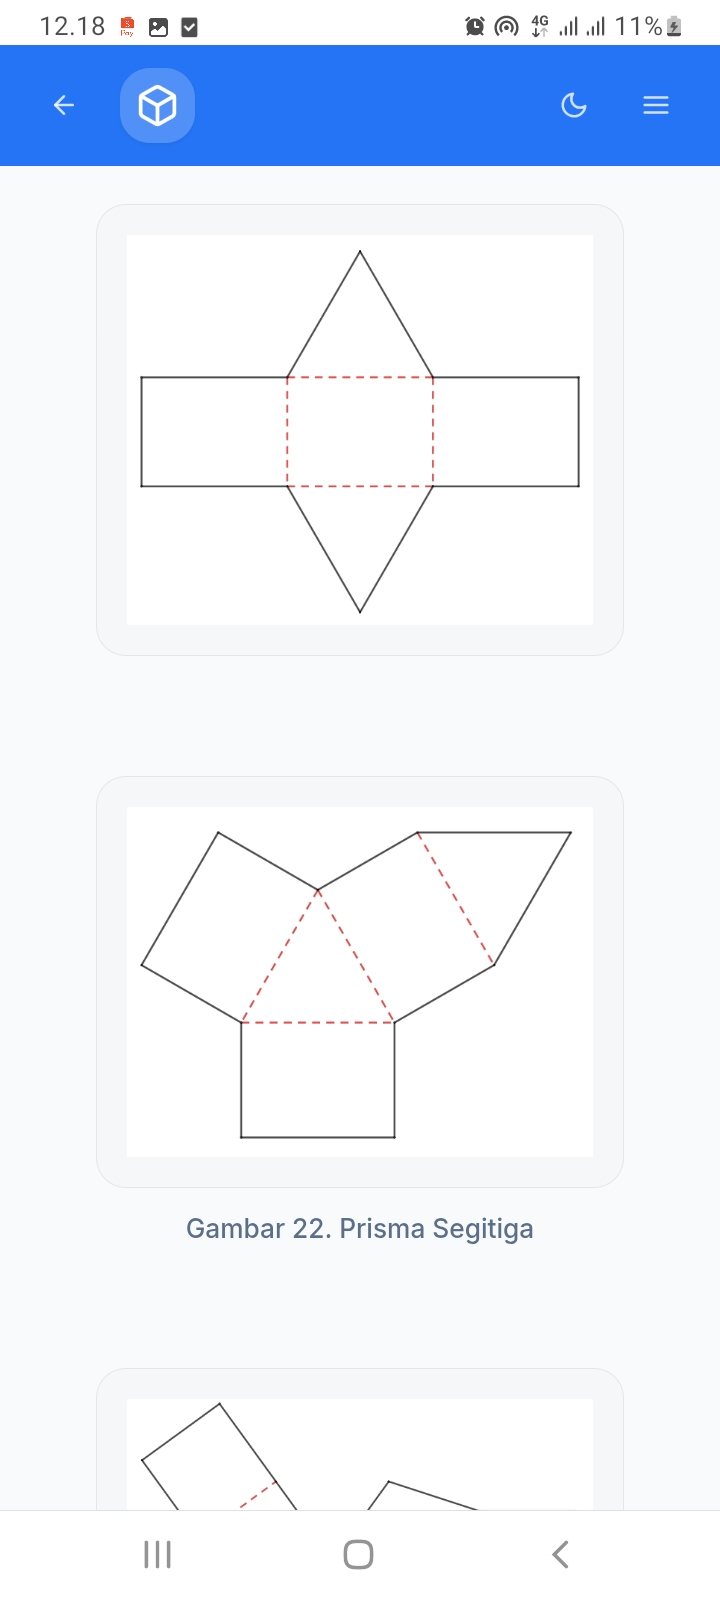
\includegraphics[width=0.25\textwidth]{revisi/sebelum/sebelumF.jpg} &
                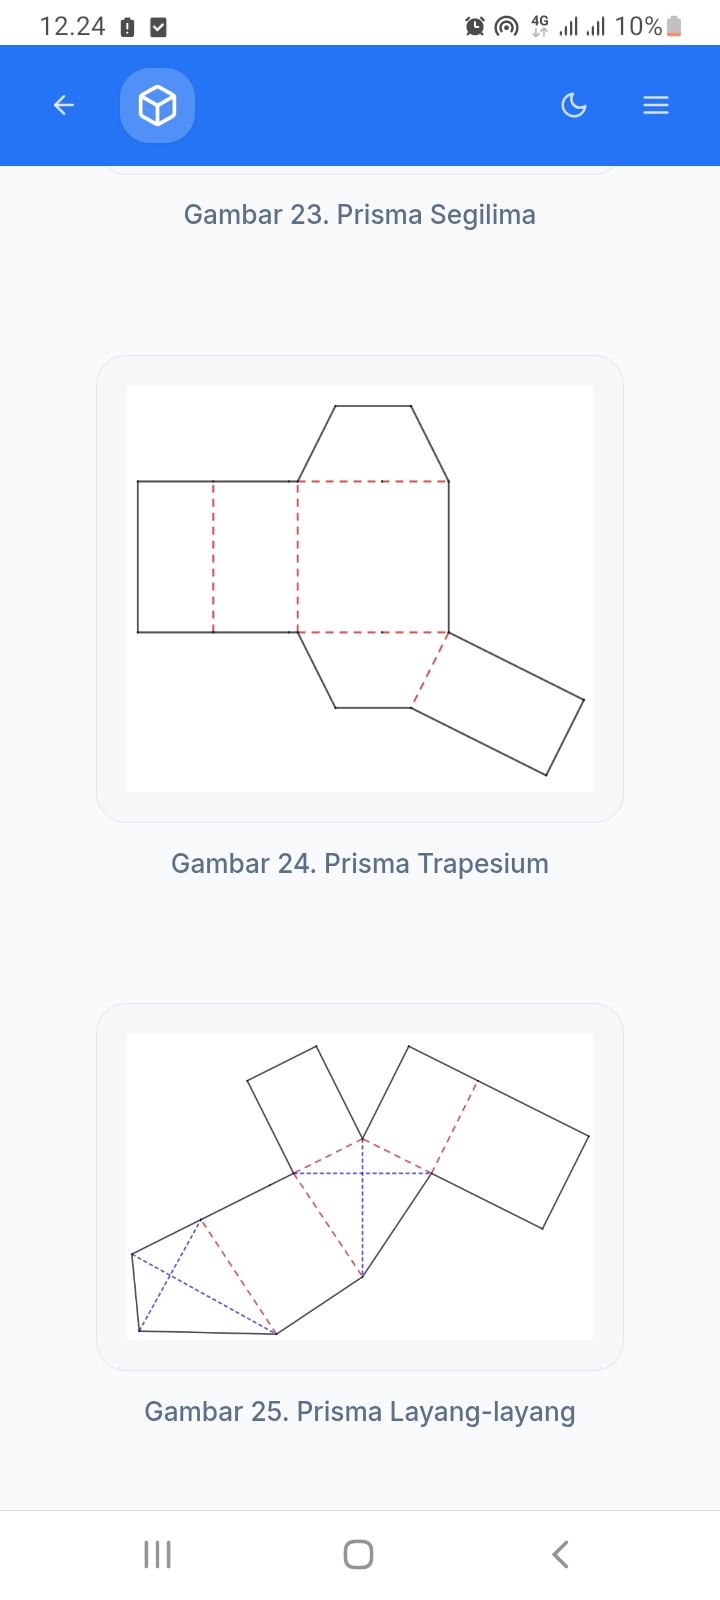
\includegraphics[width=0.25\textwidth]{revisi/sesudah/sesudahF.jpg} \\
            \end{tabular}
        \end{table}
        \item Menambahkan Capaian Pembelajaran, Indikator Pencapaian Kompetensi, dan Tujuan Pembelajaran.
        \begin{table}[H]
            \centering
            \begin{tabular}{c c c}
                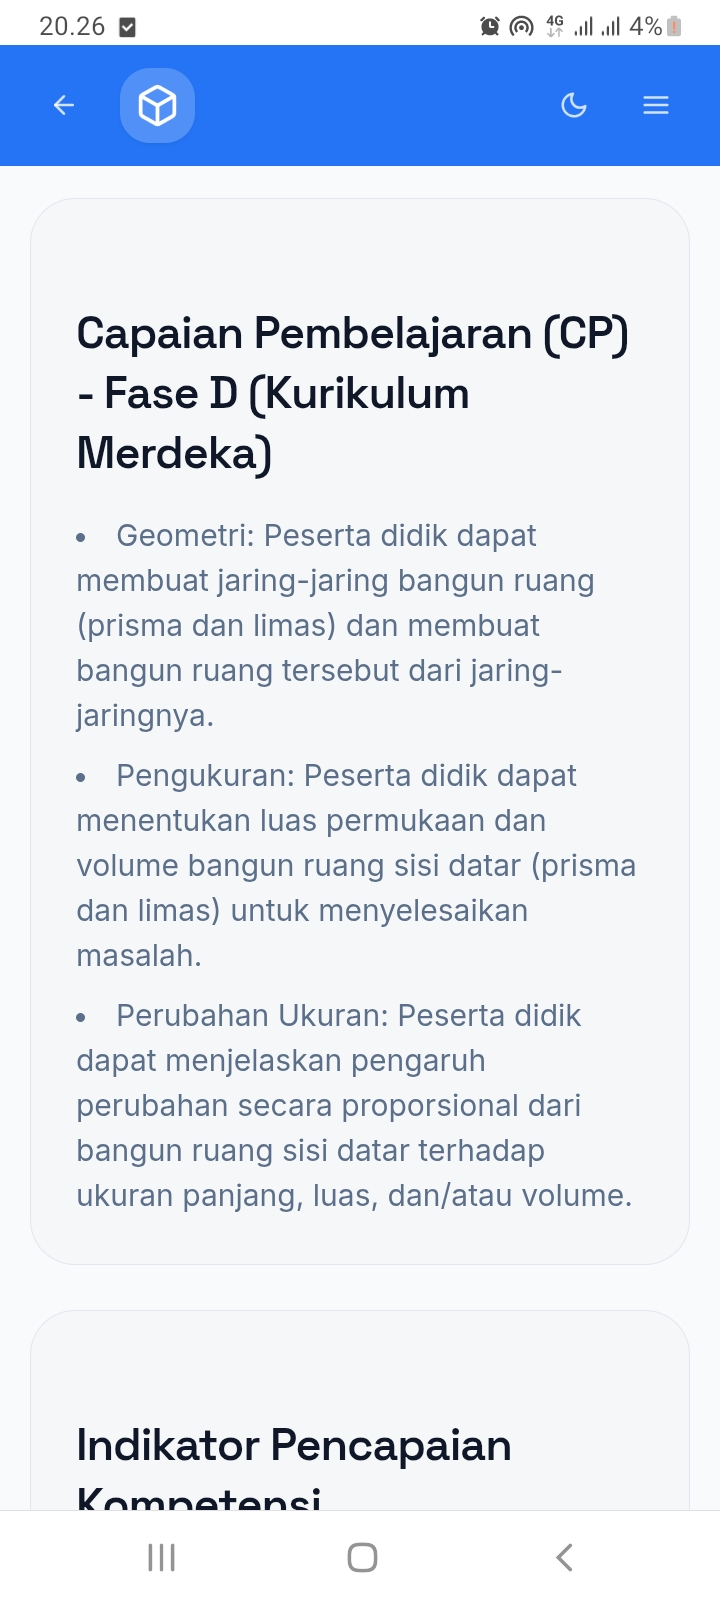
\includegraphics[width=0.25\textwidth]{revisi/sesudah/sesudahG1.jpg} &
                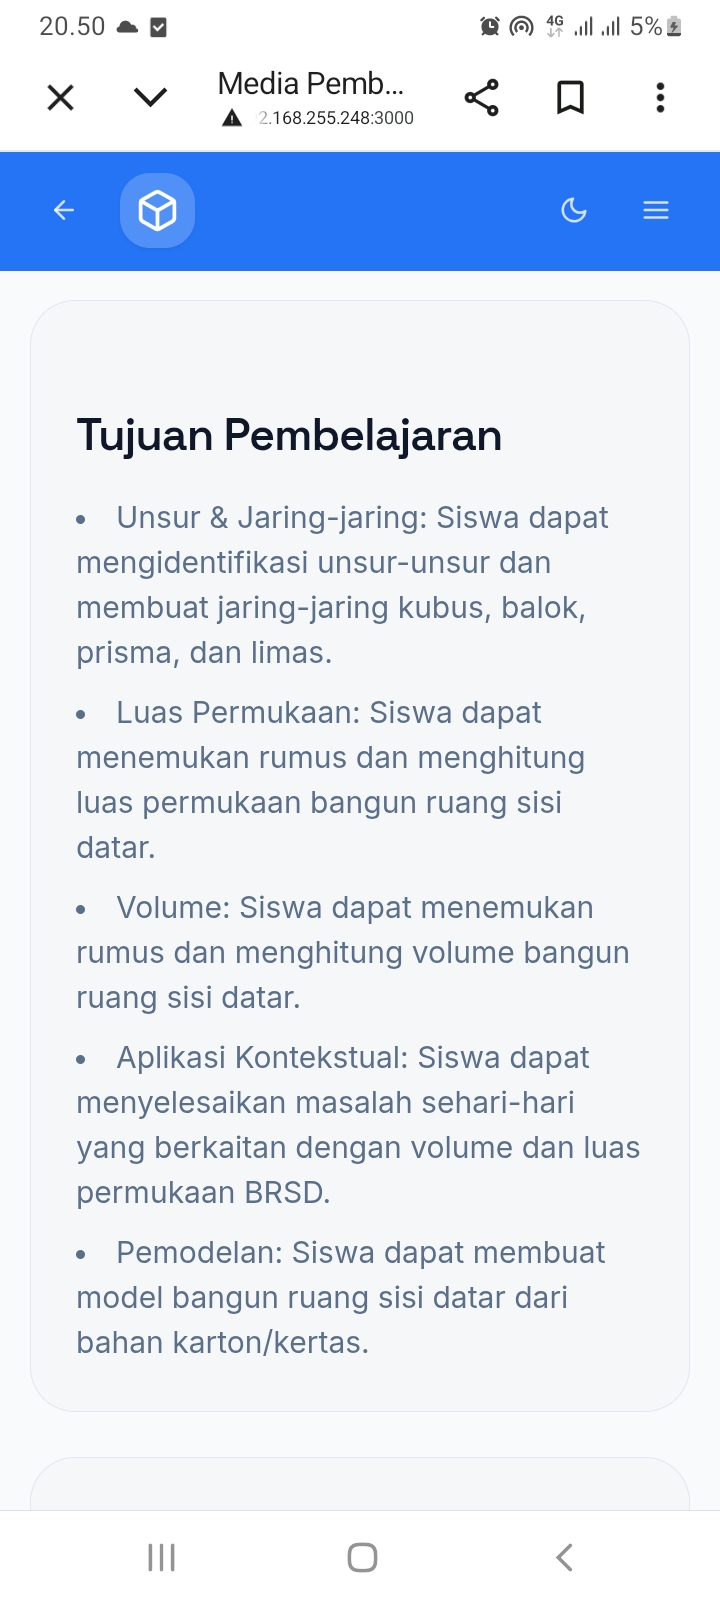
\includegraphics[width=0.25\textwidth]{revisi/sesudah/sesudahG2.jpg} &
                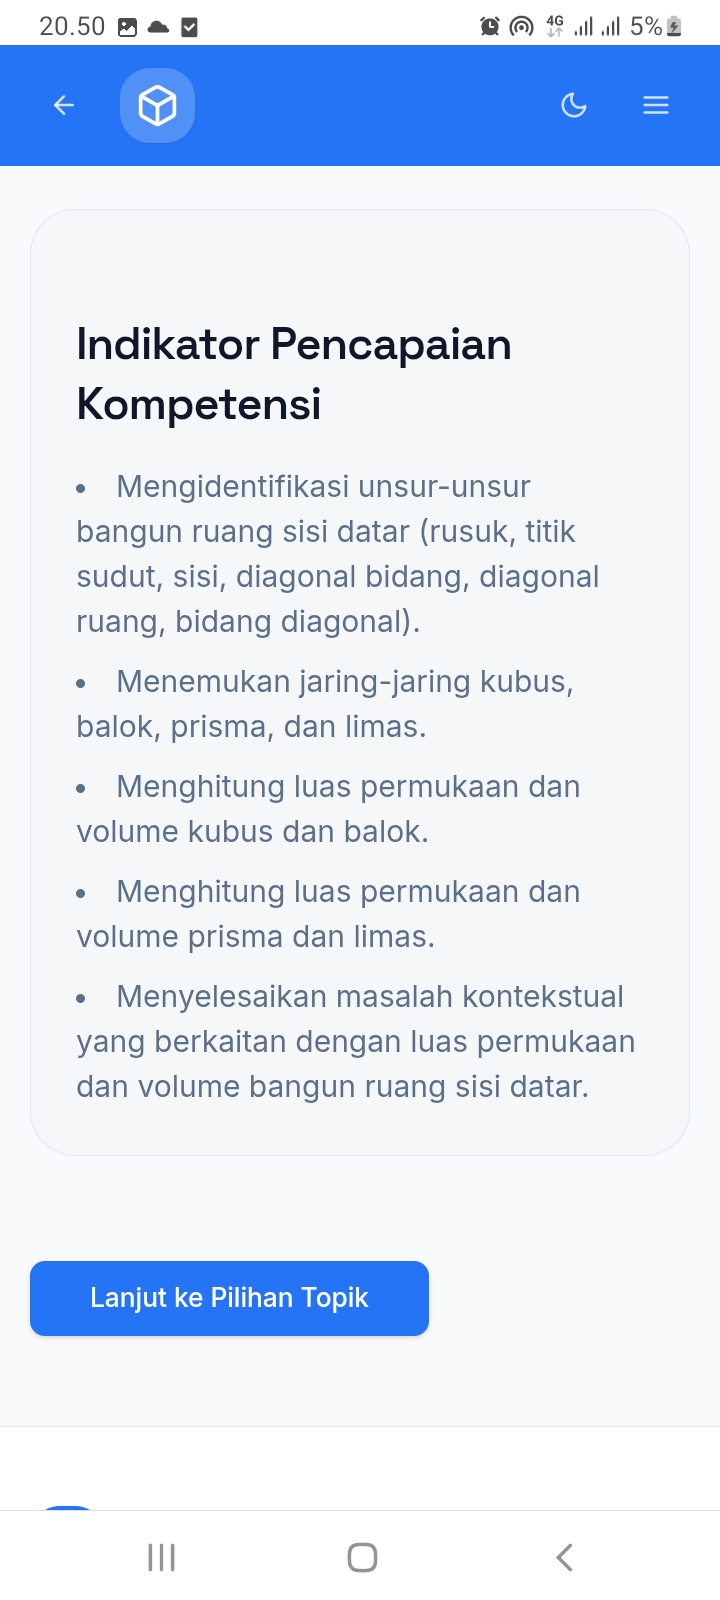
\includegraphics[width=0.25\textwidth]{revisi/sesudah/sesudahG3.jpg} \\
            \end{tabular}
        \end{table}
    \end{enumerate}
    \item Revisi Produk Hasil Validasi Ahli Media\\
    \hspace*{1cm}Revisi yang diberikan oleh ahli media tidak begitu banyak, hanya berfokus pada kunci jawaban banyak yang masih salah. Hasil perbaikan tersebut disajikan sebagai berikut.
    \begin{enumerate}
        \item Memperbaiki kunci jawaban.

         \begin{figure}[H]
            \centering
            \begin{tabular}{c c c}
                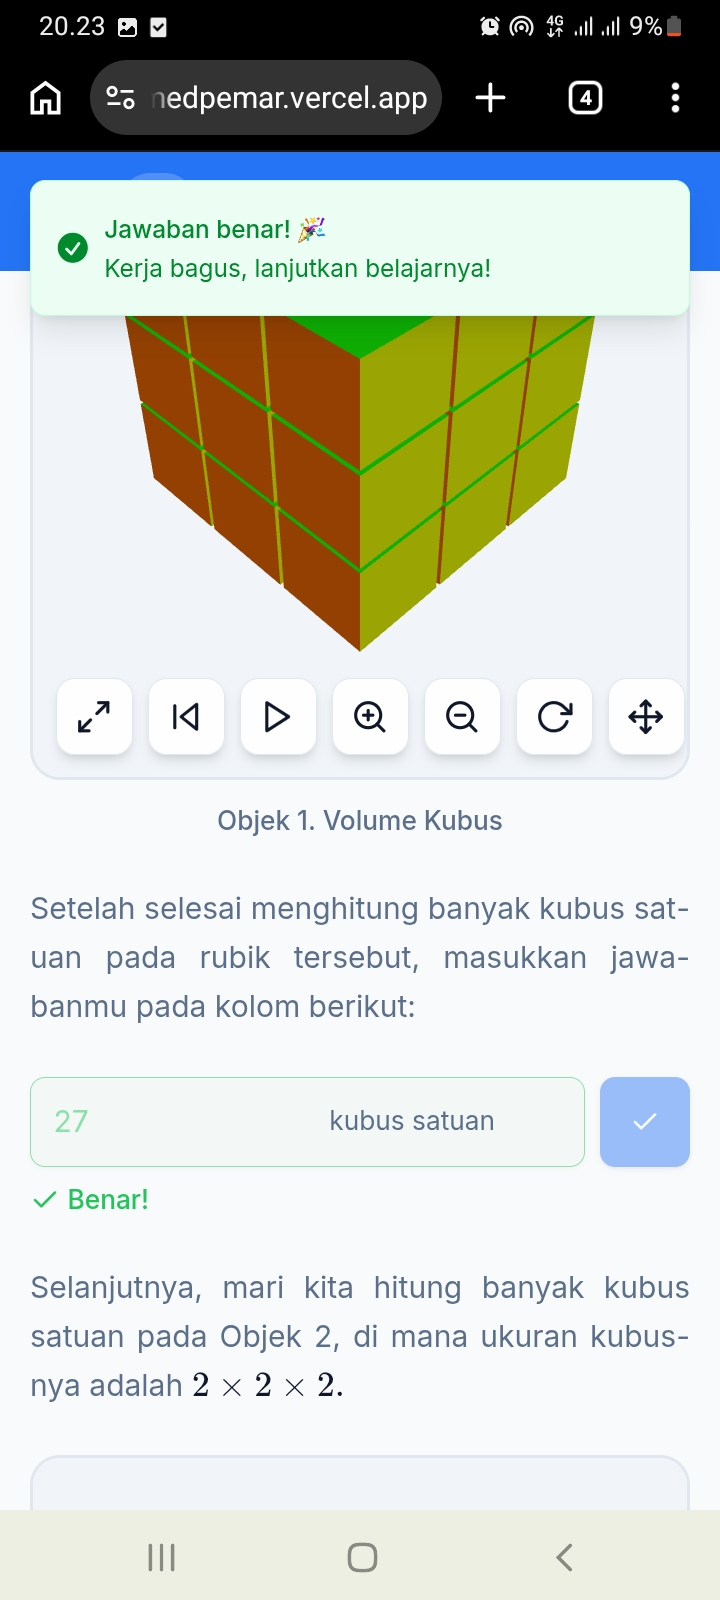
\includegraphics[width=0.25\textwidth]{revisi/Revisimedia2.jpg} &
                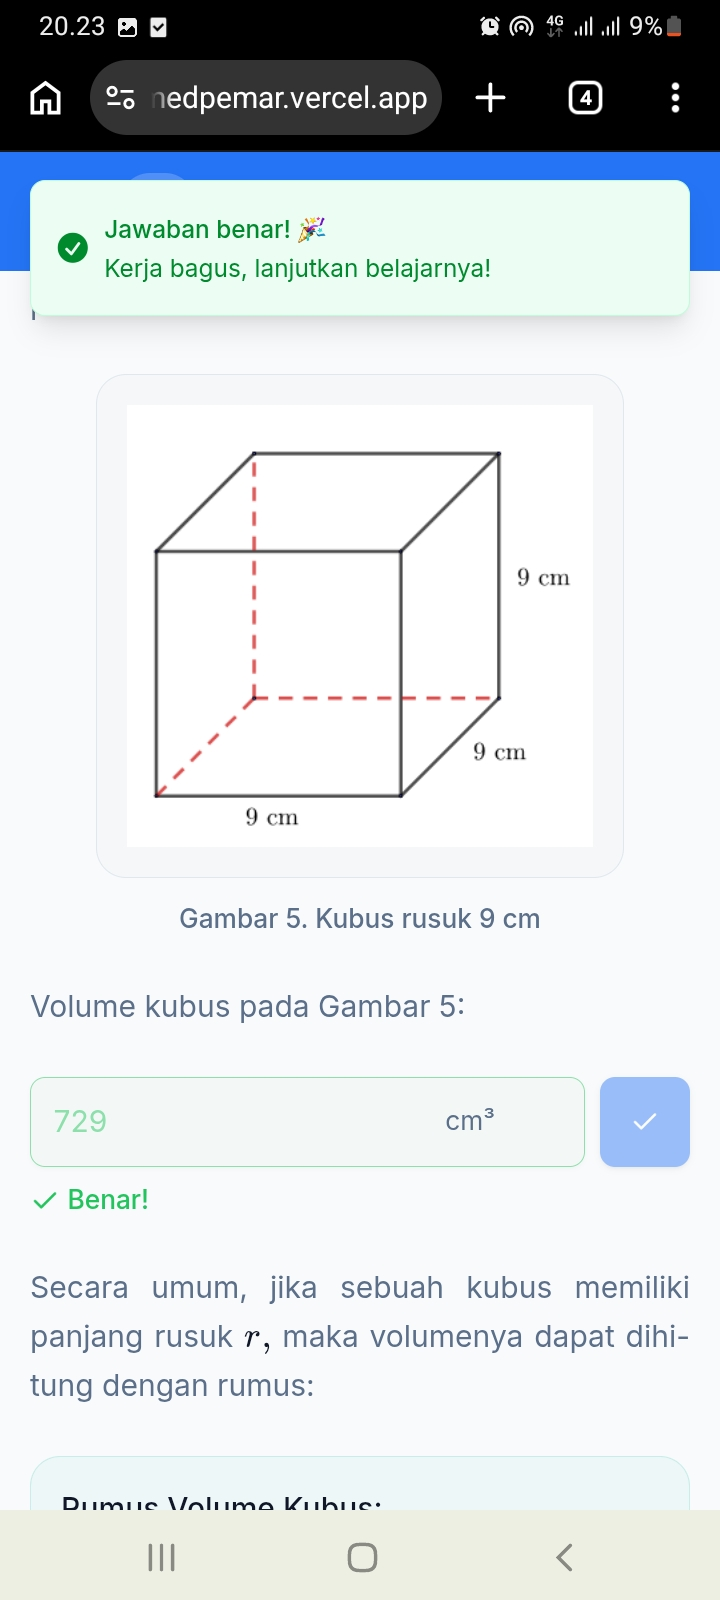
\includegraphics[width=0.25\textwidth]{revisi/Revisimedia.jpg} &
            \end{tabular}
                \caption{Contoh Perbaikan pada Kunci Jawaban}

        \end{figure}

    \end{enumerate}

    \item Revisi Produk Hasil Uji Coba Kelas Kecil
    \item Revisi Produk Hasil Uji Coba Kelas Besar
\end{enumerate}

\textbf{D. Kajian Produk Akhir}
\addcontentsline{toc}{section}{D. Kajian Produk Akhir}

\hspace*{1cm}Media pembelajaran yang dikembangkan oleh peneliti disusun dengan isi sebagaimana sebuah website pada umumnya. Dimana media pembelajaran memiliki halaman awal \textit{(Landing Page)}, halaman menu, halaman petunjuk, halaman materi, dan halaman kuis. Beikut adalah penjelasan dan tampilan dari masing-masing halaman tersebut.
\begin{enumerate}
    \item Halaman Awal\\
    \hspace*{1cm}Halaman awal merupakan halaman pertama yang dikunjungi saat siswa mengakses tautan media pembelajaran di https://medpemar.vercel.app. Pada halaman ini siswa akan melihat judul media pembelajaran, penjelasan singkat terkait media, cakupan isi media, dan instansi pembuat media. Berikut tampilan halaman awal pada mode ponsel dan mode layar lebar/komputer.
    \begin{figure}[H]
            \centering
            \begin{tabular}{c c c}
                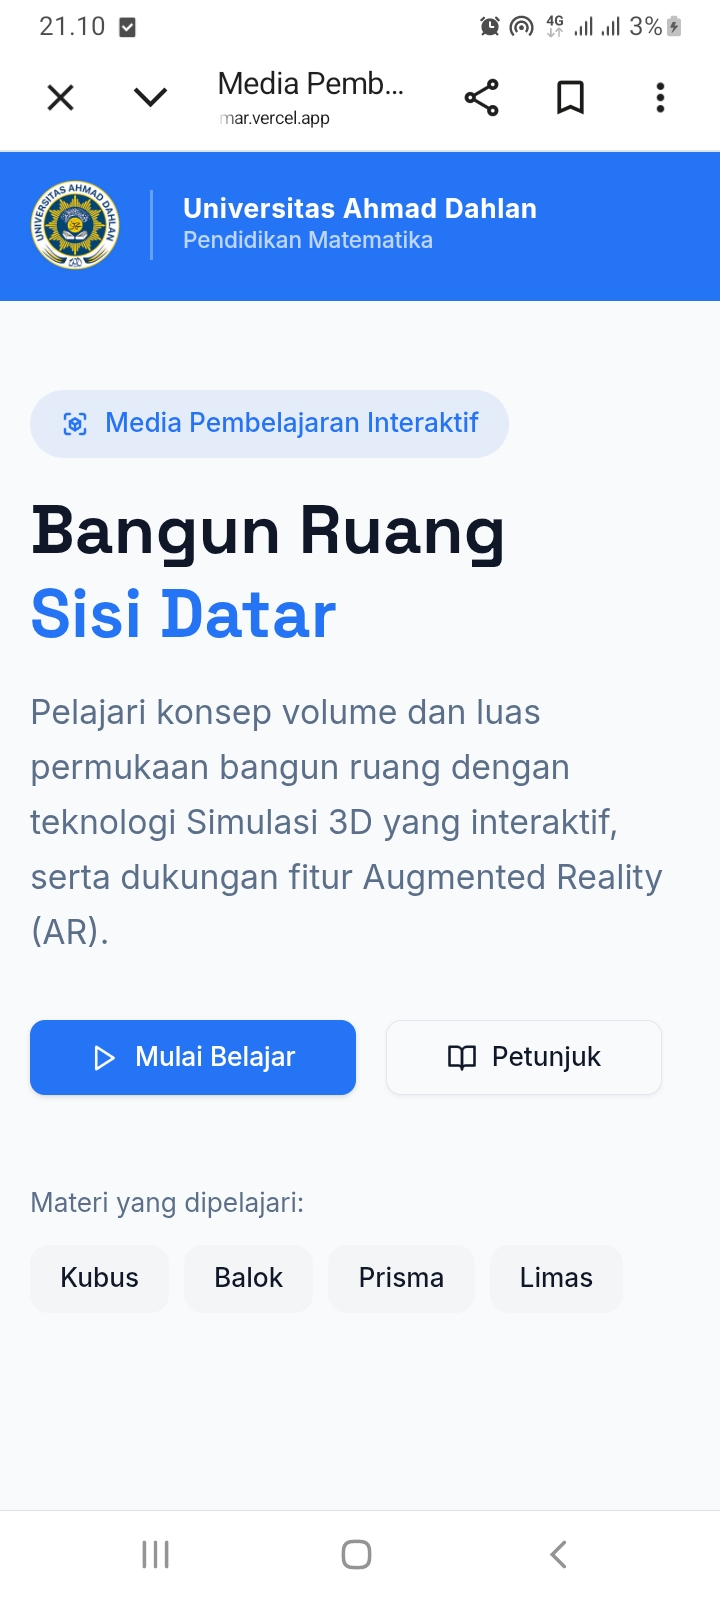
\includegraphics[width=0.25\textwidth]{revisi/Landingpage1.jpg} &
                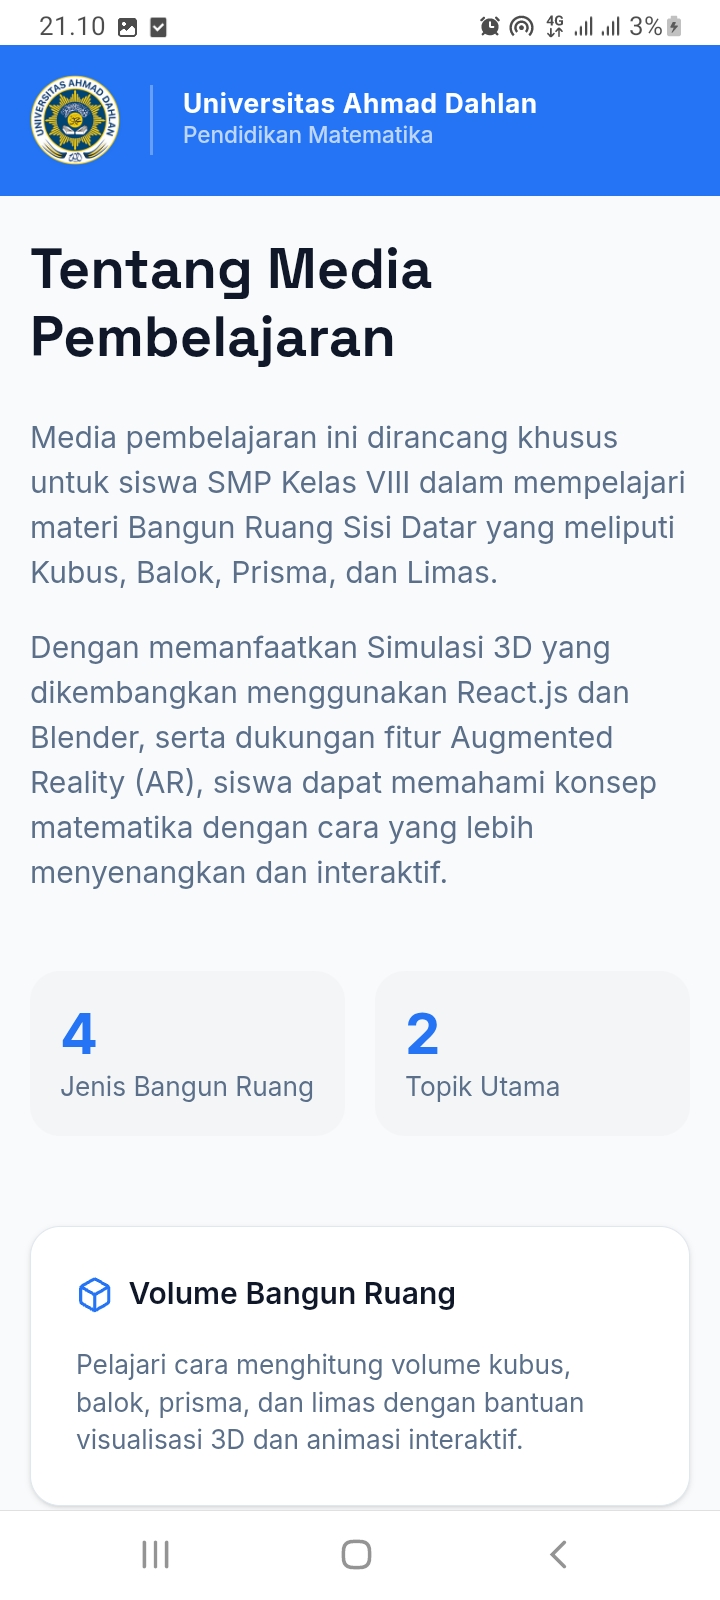
\includegraphics[width=0.25\textwidth]{revisi/Landingpage2.jpg} &
            \end{tabular}
                \caption{Landing Page versi Mobile}

        \end{figure}
        \begin{figure}[H]
            \centering
            \begin{tabular}{c c c}
                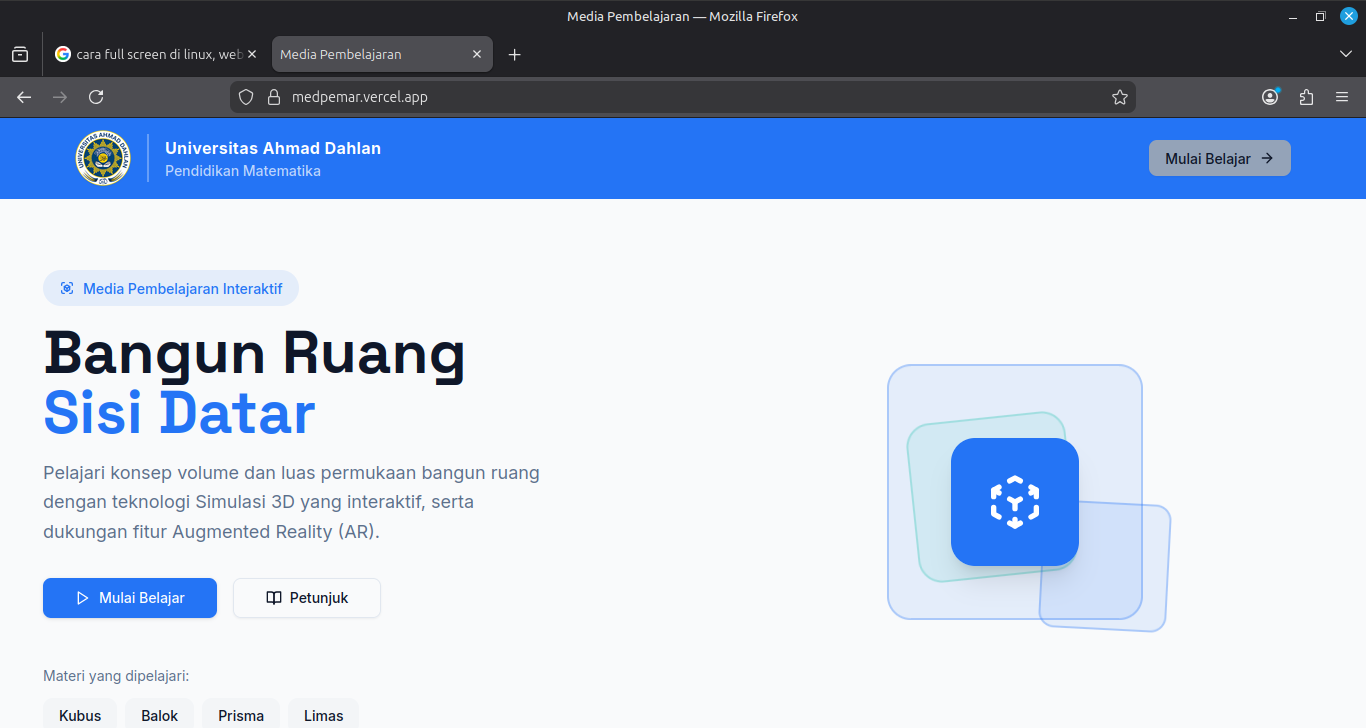
\includegraphics[width=1\textwidth]{revisi/Landingpage3.png} &
            \end{tabular}
                \caption{Landing Page versi Desktop}

        \end{figure}
    \item Halaman Pendahuluan Pembelajaran\\
    \hspace*{1cm}Halaman ini berisi tentang tujuan pembelajaran, capaian pembelajaran, dan indikator pencapaian kompetensi yang akan dipelajari oleh peserta didik.
    \begin{figure}[H]
            \centering
            \begin{tabular}{c c c}
                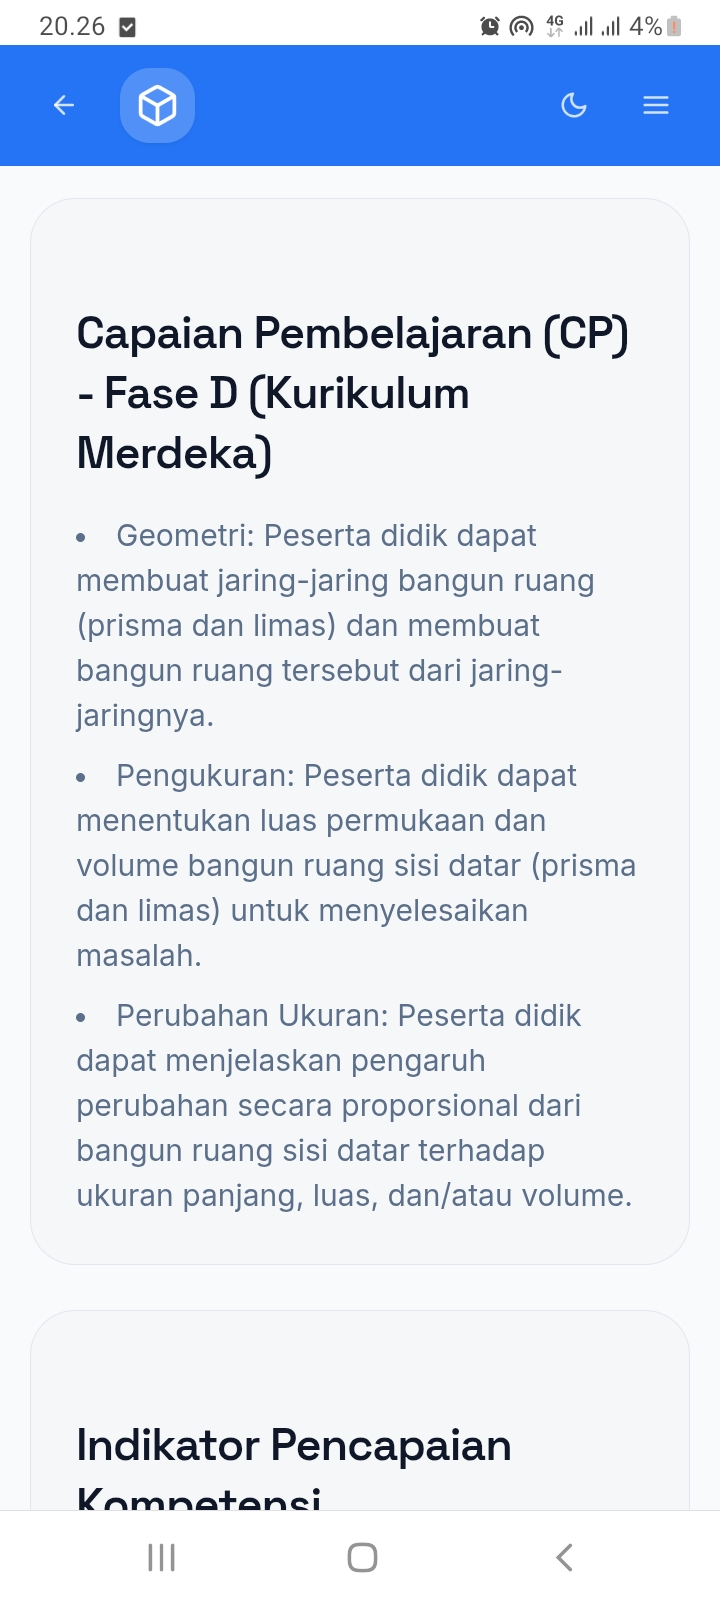
\includegraphics[width=0.3\textwidth]{revisi/sesudah/sesudahG1.jpg} &
                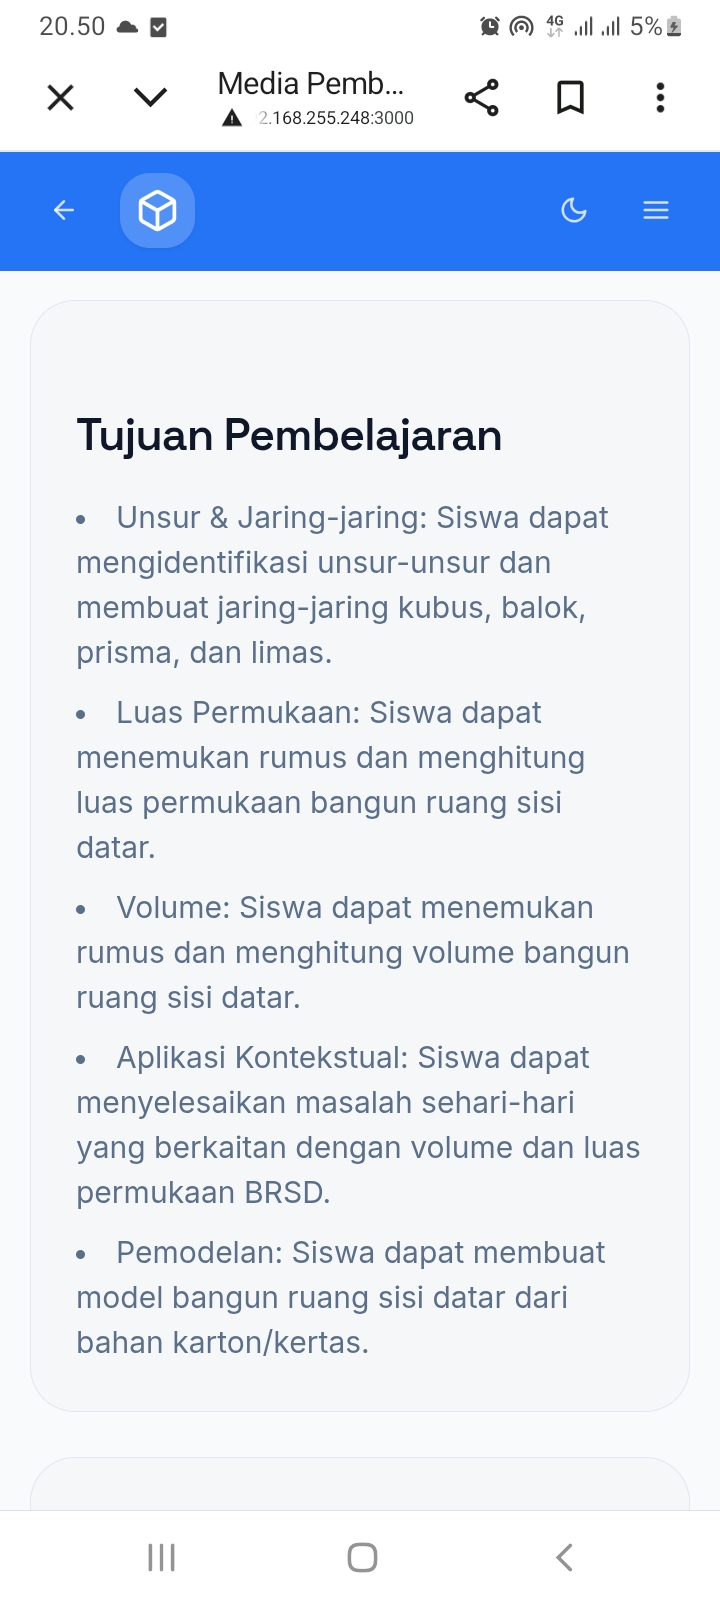
\includegraphics[width=0.3\textwidth]{revisi/sesudah/sesudahG2.jpg} &
                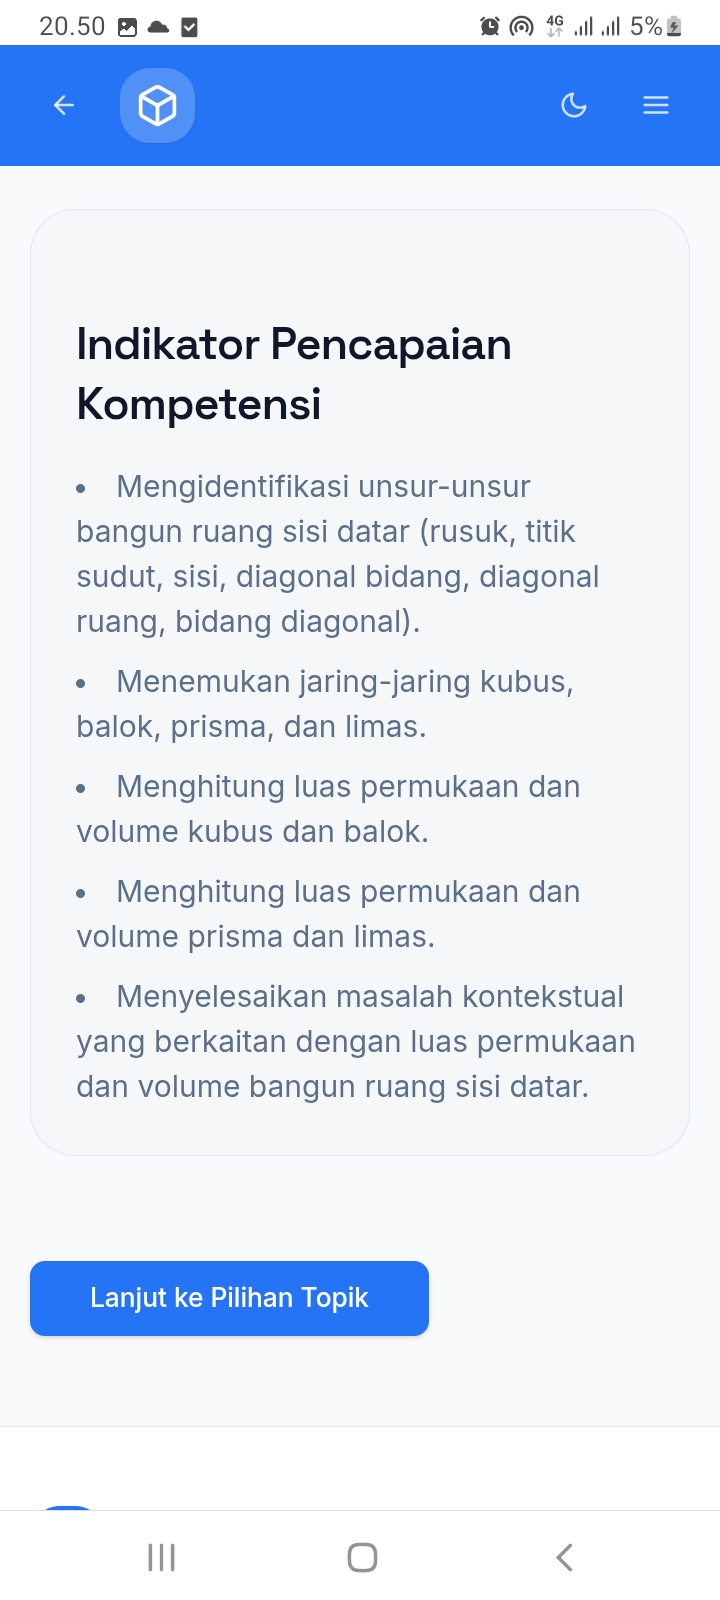
\includegraphics[width=0.3\textwidth]{revisi/sesudah/sesudahG3.jpg} \\
            \end{tabular}
                \caption{Halaman Pendahuluan Pembelajaran}

        \end{figure}
    \item Halaman Menu\\
    \hspace*{1cm}Pada halaman ini berisi pilihan materi yang akan dipelajari siswa, dan juga terdapat pilihan untuk ke halaman latihan soal. Pada halaman ini siswa juga bisa mengunduh barcode yang digunakan untuk menampilkan simulasi 3D.
    \begin{figure}[H]
            \centering
            \begin{tabular}{c c c}
                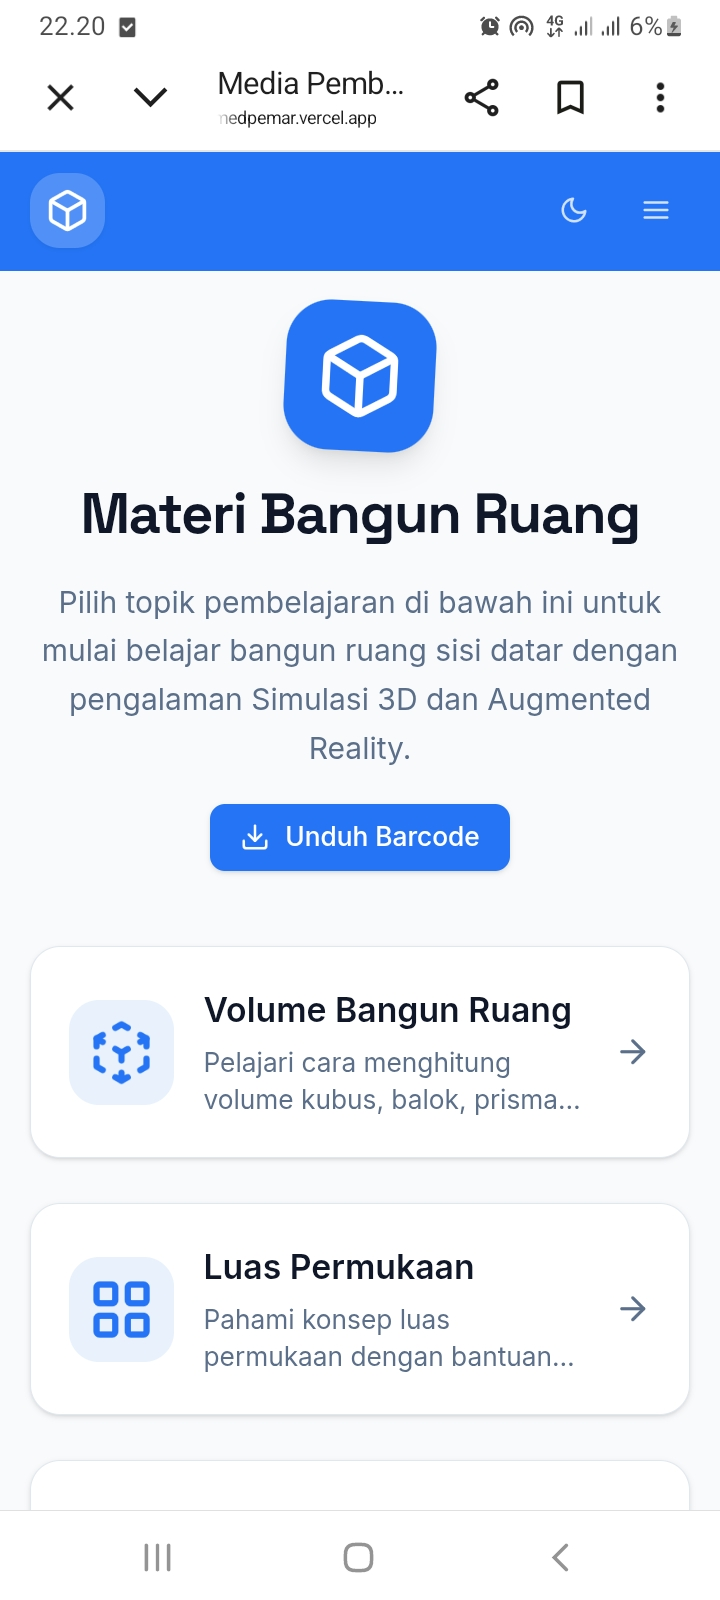
\includegraphics[width=0.3\textwidth]{revisi/Menu.jpg} &
                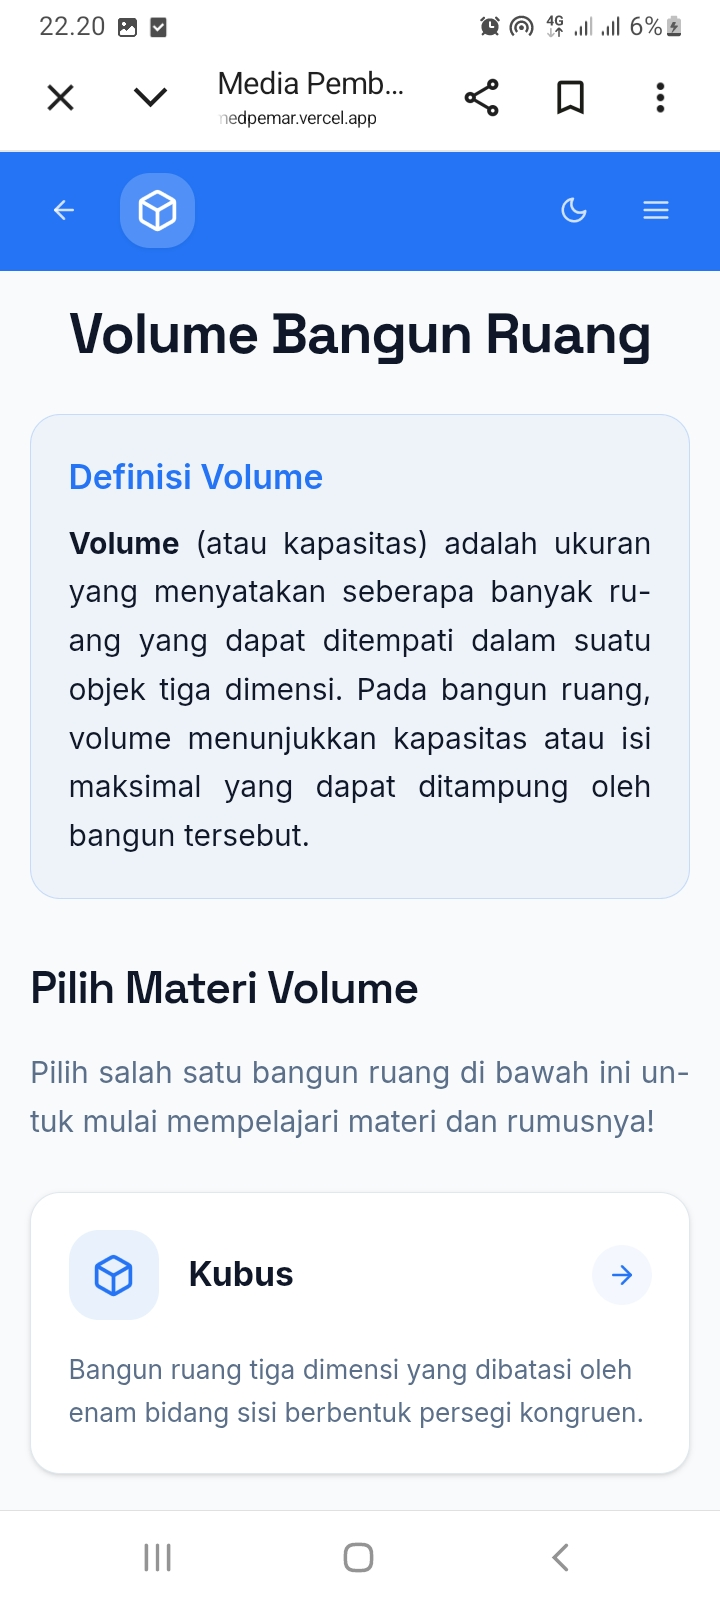
\includegraphics[width=0.3\textwidth]{revisi/Menuvolume.jpg} &
                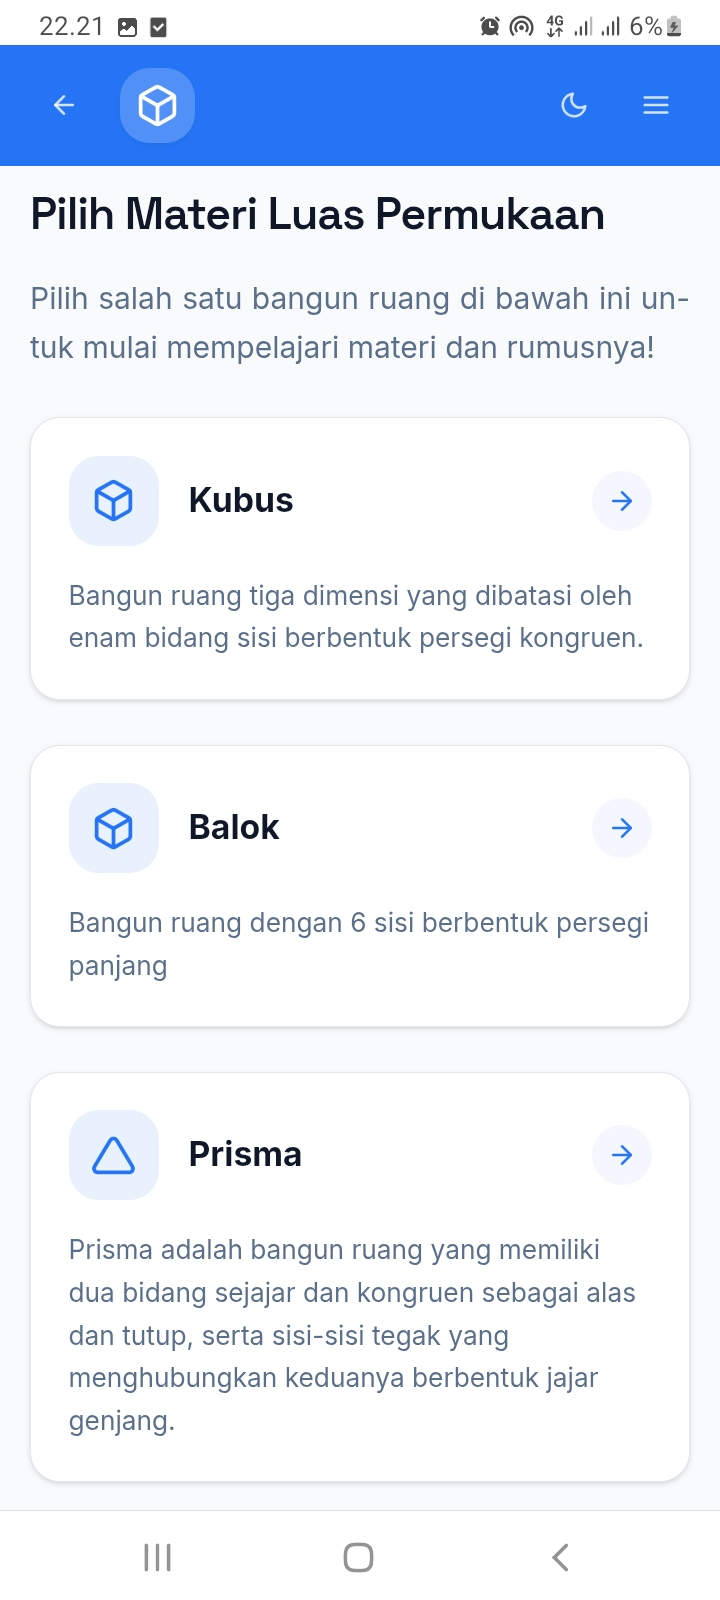
\includegraphics[width=0.3\textwidth]{revisi/Menuluaspermukaan.jpg} \\
            \end{tabular}
                \caption{Halaman Menu}

        \end{figure}

    \item Halaman Materi\\
    \hspace*{1cm}Pada halaman materi, peserta didik akan mempelajari dua topik utama, yaitu volume dan luas permukaan bangun ruang. Peserta didik akan melihat bangun ruang yang disajikan dalam bentuk 3D dan simulasi 3D. Bangun ruang tersebut juga dapat dianimasikan untuk mempermudah pemahaman. Untuk mengevaluasi pemahaman peserta didik, tersedia latihan soal dan pembahasan di akhir setiap bab.
    \begin{figure}[H]
        \centering
        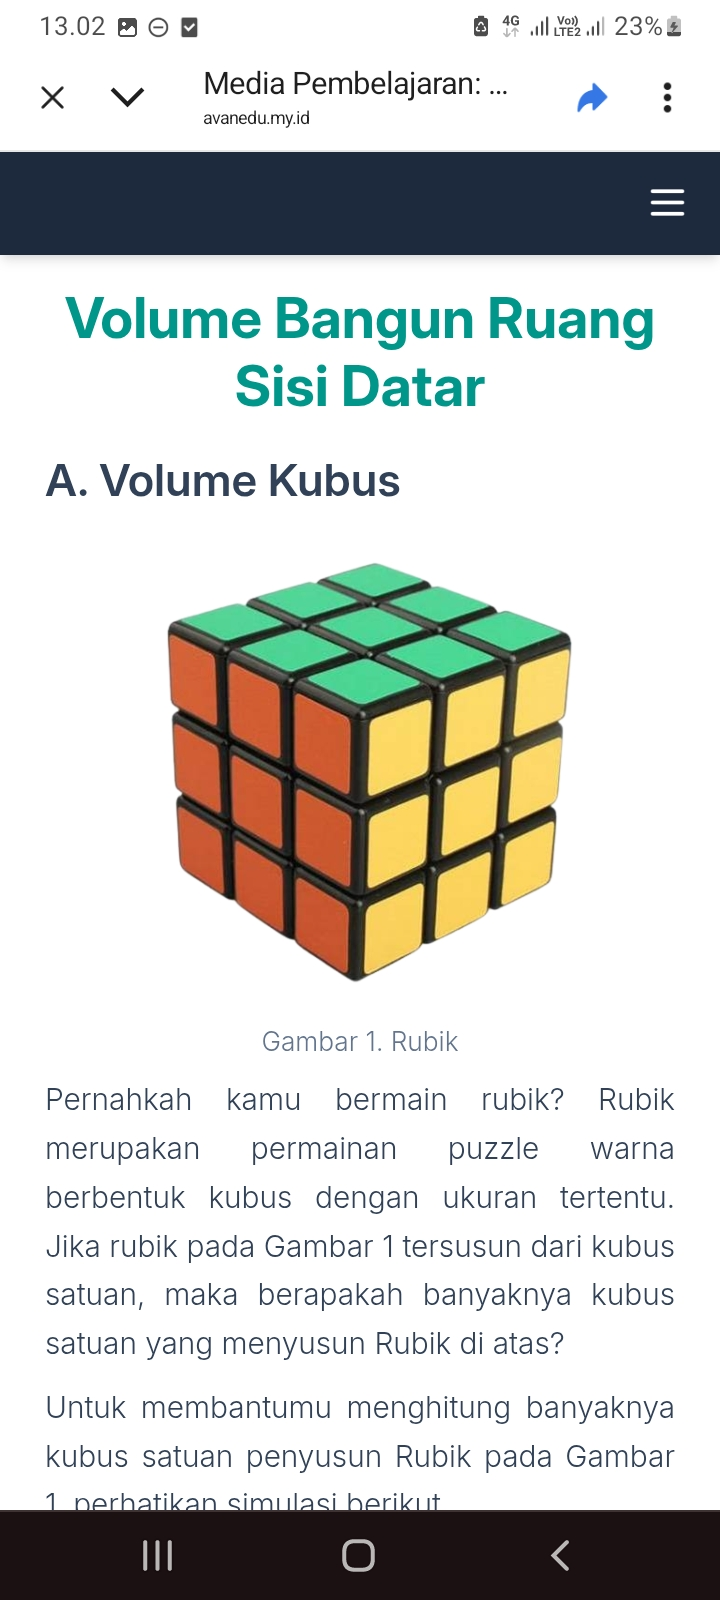
\includegraphics[width=0.2\textwidth]{images/materi1.jpg}
        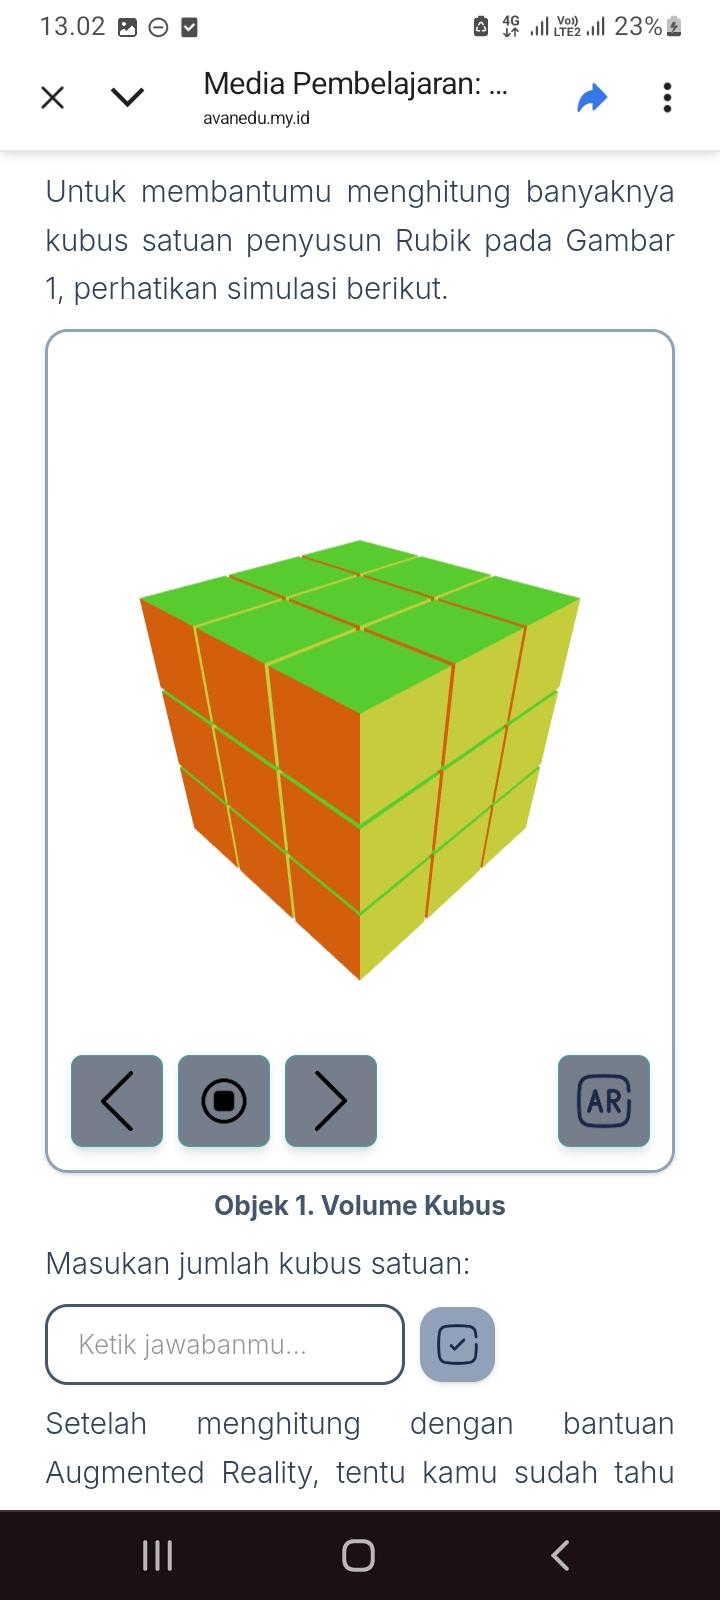
\includegraphics[width=0.2\textwidth]{images/materi2.jpg}
        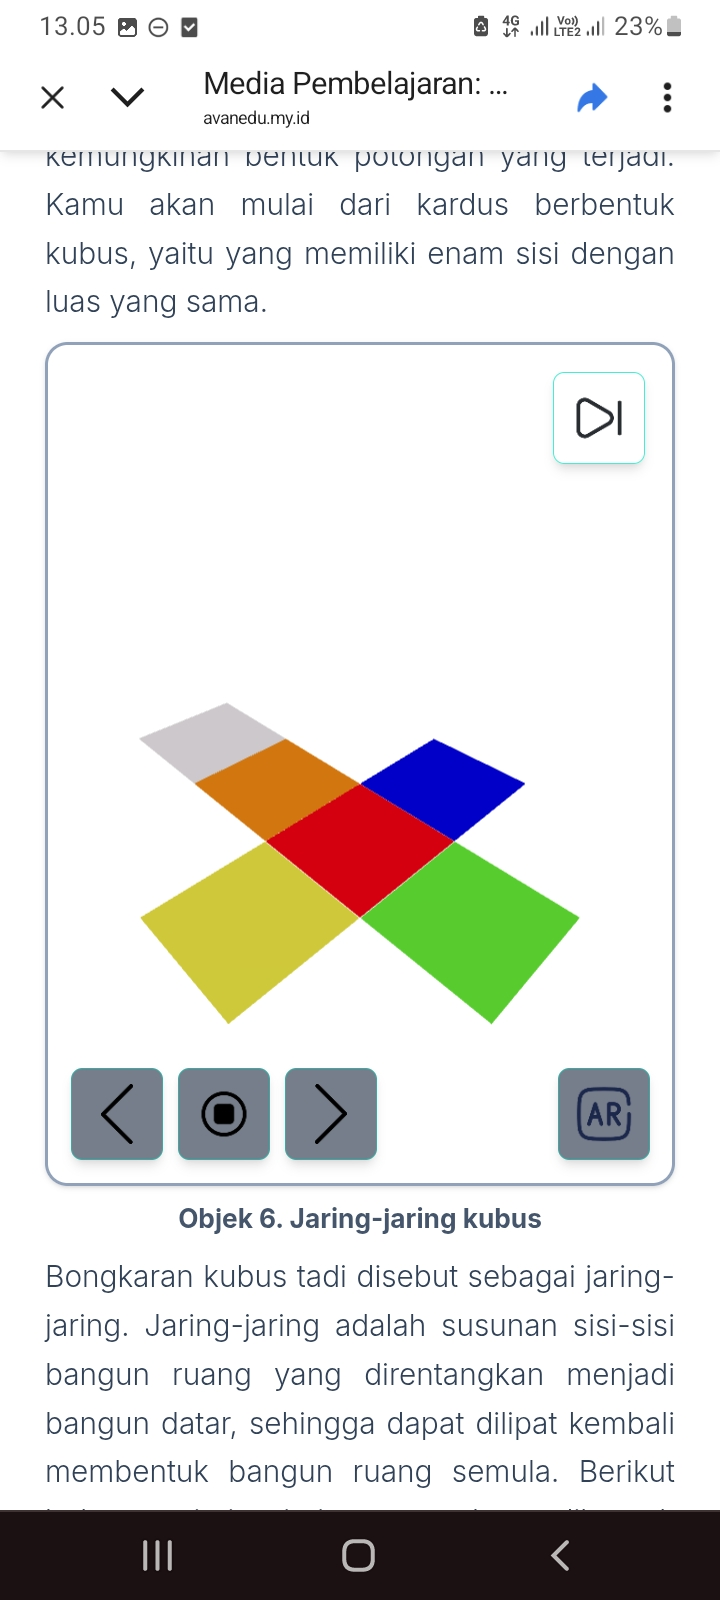
\includegraphics[width=0.2\textwidth]{images/materi3.jpg}
        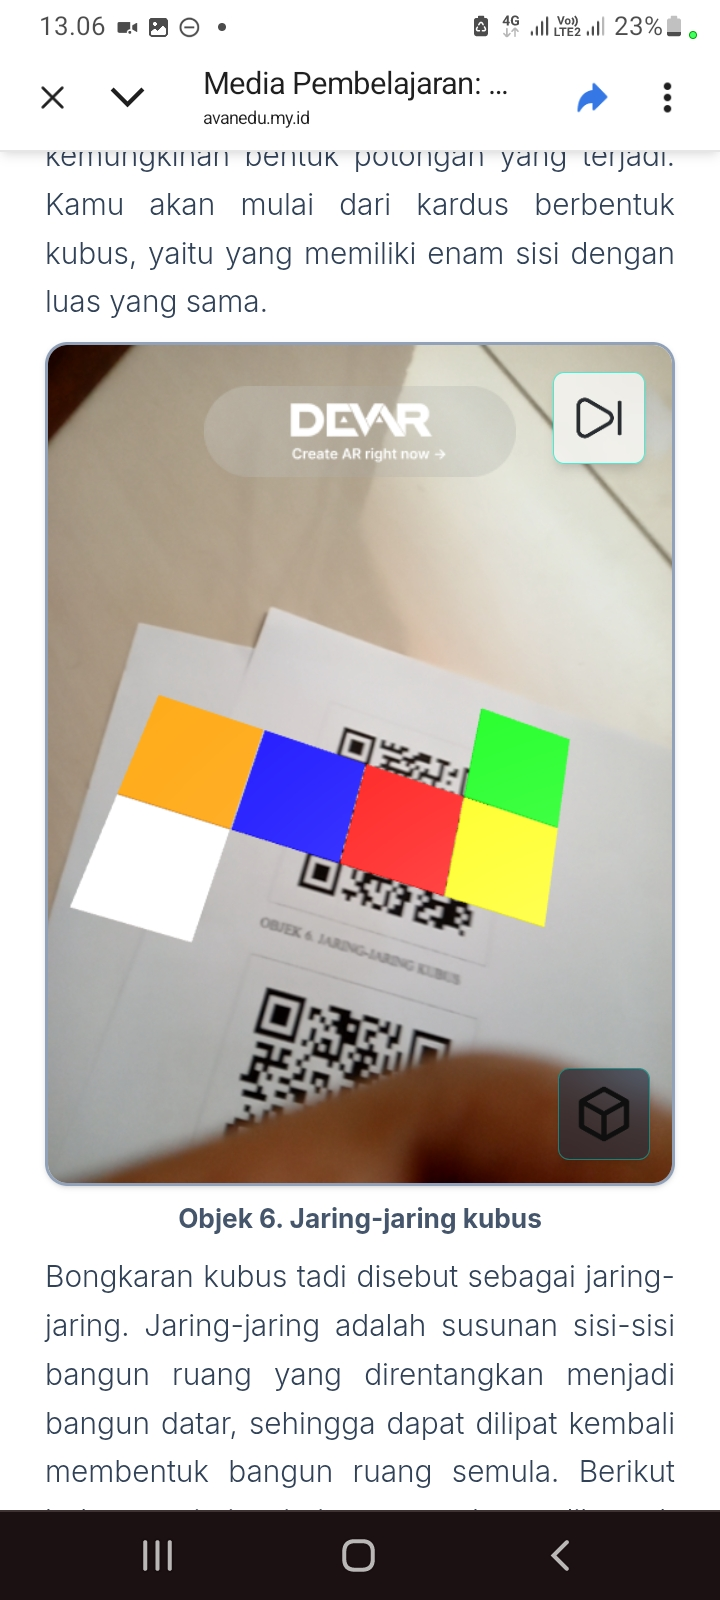
\includegraphics[width=0.2\textwidth]{images/materi4.jpg}
        \caption{Halaman Materi}
        \label{fig:materi}
    \end{figure}

    \item Halaman Kuis\\
    \hspace*{1cm}Pada halaman kuis, disajikan lima soal yang sesuai dengan latihan soal di akhir setiap bab. Terdapat juga penghitung waktu (timer) dengan batas waktu pengerjaan selama 30 menit. Untuk mulai mengerjakan kuis, peserta didik perlu memasukkan kode ujian. Peserta didik dapat menjawab soal dengan mengisi kolom jawaban yang disediakan, serta dapat menyisipkan foto untuk memperkuat jawabannya.
    \begin{figure}[H]
        \centering
        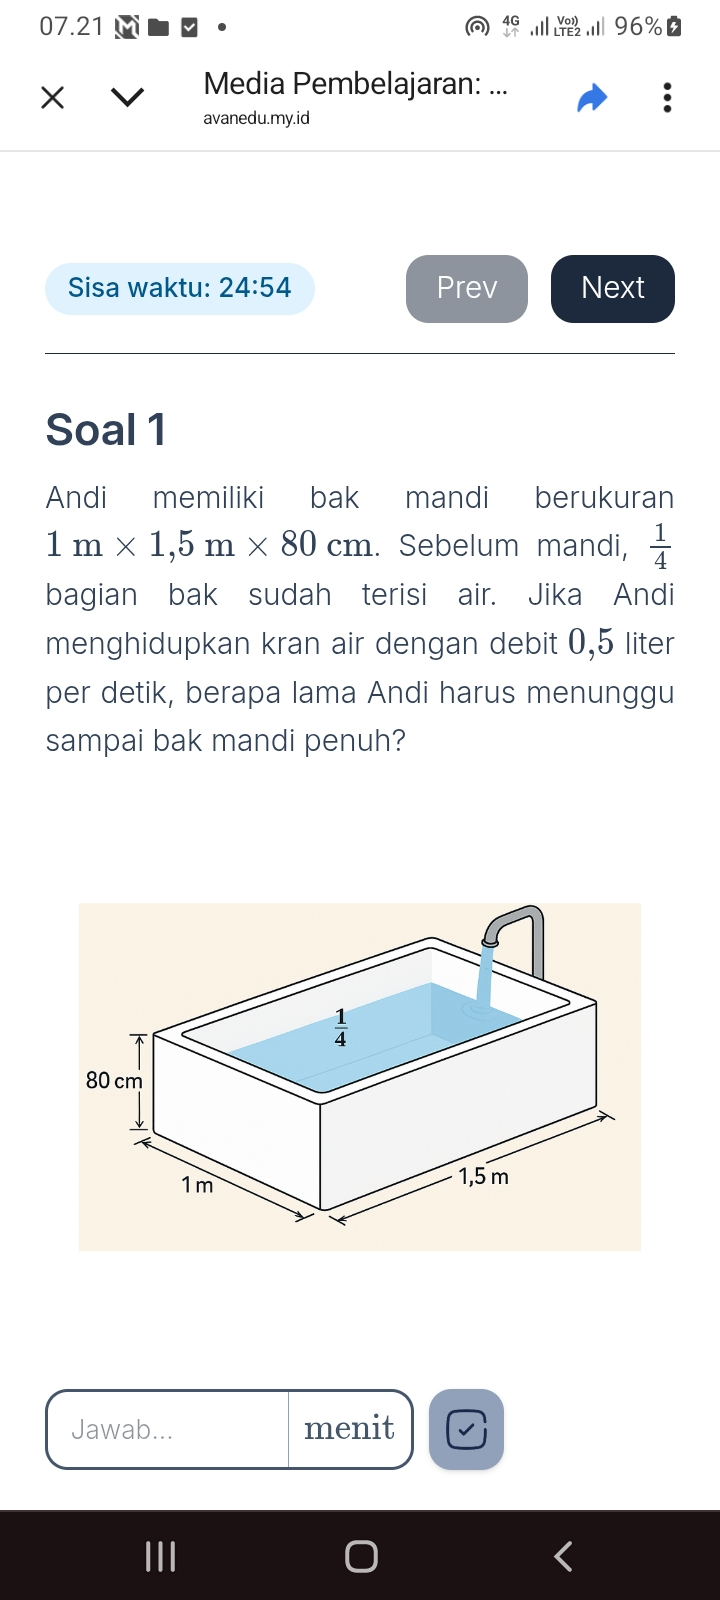
\includegraphics[width=0.25\textwidth]{images/kuis1.jpg}
        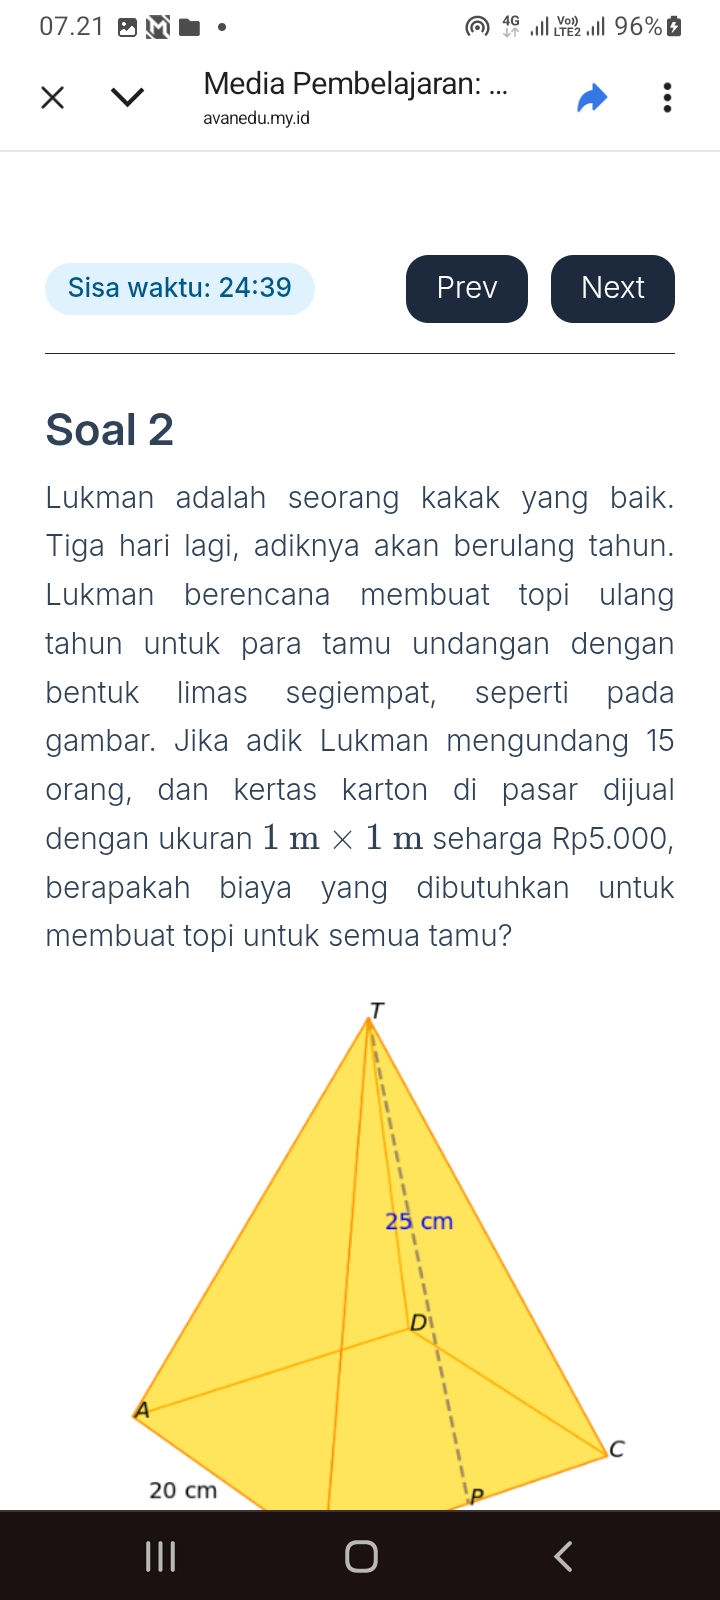
\includegraphics[width=0.25\textwidth]{images/kuis2.jpg}
        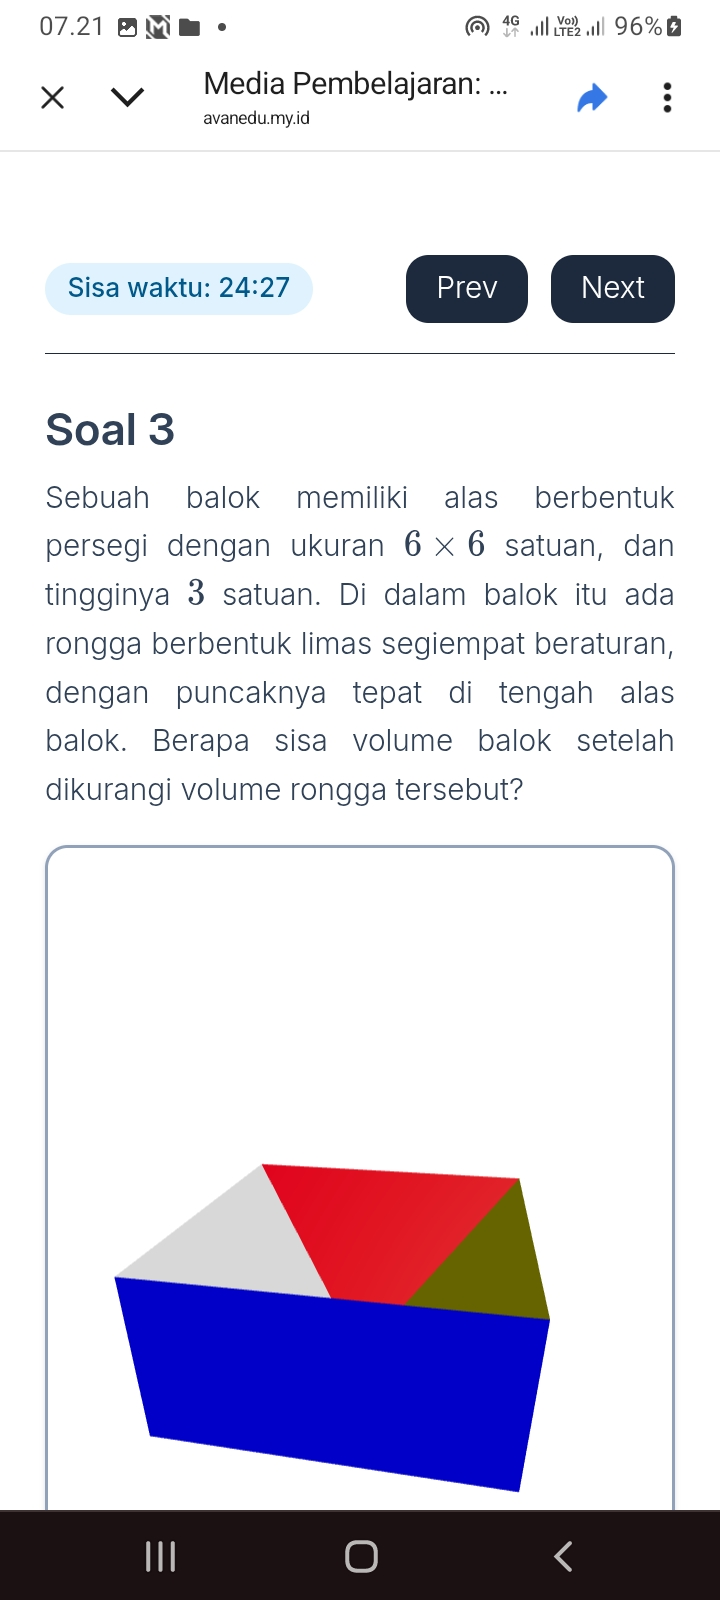
\includegraphics[width=0.25\textwidth]{images/kuis3.jpg}
        \caption{Halaman Kuis}
        \label{fig:kuis}
    \end{figure}

\end{enumerate}